\documentclass[a4paper,9pt]{article}
%\documentclass{aa}
%\pgfplotsset{compat=1.12}
\usepackage{conference}
\usepackage{latexsym}
\usepackage[perpage,symbol*]{footmisc}
%\usepackage[utf8]{inputenc}
\usepackage[utf8x]{inputenc}
\usepackage{textcomp}
\usepackage[english]{babel}
\usepackage{amssymb,amsfonts,amsmath}
\usepackage{xcolor}
\usepackage{tikz}
\usepackage{tikz-3dplot}
\usepackage{tikz-feynman}
\usepackage{pgfplots}
\usepackage{pgfplotstable}
\usepackage{cite}
\usepackage{hyperref}
\usepackage[varg]{txfonts}
\usepackage{booktabs}       
\usepackage{tabularx}
\usepackage{enumerate}

\usepackage{multicol}

\usepackage{etoolbox}

\usetikzlibrary{patterns,arrows.meta,shapes,calc,angles,positioning,intersections,through,quotes,decorations.markings,shadows.blur,decorations.pathreplacing}
\tdplotsetmaincoords{70}{110}
\usepackage{tkz-euclide}
\usetkzobj{all}
\def\doubleunderline#1{\underline{\underline{#1}}}
\newcounter{row}
\newcounter{col}
\newcommand\setrow[9]{
  \setcounter{col}{1}
  \foreach \n in {#1, #2, #3, #4, #5, #6, #7, #8, #9} {
    \edef\x{\value{col} - 0.5}
    \edef\y{9.5 - \value{row}}
    \node[anchor=center] at (\x, \y) {\n};
    \stepcounter{col}
  }
  \stepcounter{row}
}

\tikzset{%
        brace/.style = { decorate, decoration={brace, amplitude=5pt} },
       mbrace/.style = { decorate, decoration={brace, amplitude=5pt, mirror} },
        label/.style = { black, midway, scale=0.5, align=center },
     toplabel/.style = { label, above=.5em, anchor=south },
    leftlabel/.style = { label,rotate=-90,left=.5em,anchor=north },   
  bottomlabel/.style = { label, below=.5em, anchor=north },
        force/.style = { rotate=-90,scale=0.4 },
        round/.style = { rounded corners=2mm },
       legend/.style = { right,scale=0.4 },
        nosep/.style = { inner sep=0pt },
   generation/.style = { anchor=base }
}

\newcommand\particle[7][white]{%
  \begin{tikzpicture}[x=1cm, y=1cm]
    \path[fill=#1,blur shadow={shadow blur steps=5}] (0.1,0) -- (0.9,0)
        arc (90:0:1mm) -- (1.0,-0.9) arc (0:-90:1mm) -- (0.1,-1.0)
        arc (-90:-180:1mm) -- (0,-0.1) arc(180:90:1mm) -- cycle;
    \ifstrempty{#7}{}{\path[fill=purple!50!white]
        (0.6,0) --(0.7,0) -- (1.0,-0.3) -- (1.0,-0.4);}
    \ifstrempty{#6}{}{\path[fill=green!50!black!50] (0.7,0) -- (0.9,0)
        arc (90:0:1mm) -- (1.0,-0.3);}
    \ifstrempty{#5}{}{\path[fill=orange!50!white] (1.0,-0.7) -- (1.0,-0.9)
        arc (0:-90:1mm) -- (0.7,-1.0);}
    \draw[\ifstrempty{#2}{dashed}{black}] (0.1,0) -- (0.9,0)
        arc (90:0:1mm) -- (1.0,-0.9) arc (0:-90:1mm) -- (0.1,-1.0)
        arc (-90:-180:1mm) -- (0,-0.1) arc(180:90:1mm) -- cycle;
    \ifstrempty{#7}{}{\node at(0.825,-0.175) [rotate=-45,scale=0.2] {#7};}
    \ifstrempty{#6}{}{\node at(0.9,-0.1)  [nosep,scale=0.17] {#6};}
    \ifstrempty{#5}{}{\node at(0.9,-0.9)  [nosep,scale=0.2] {#5};}
    \ifstrempty{#4}{}{\node at(0.1,-0.1)  [nosep,anchor=west,scale=0.25]{#4};}
    \ifstrempty{#3}{}{\node at(0.1,-0.85) [nosep,anchor=west,scale=0.3] {#3};}
    \ifstrempty{#2}{}{\node at(0.1,-0.5)  [nosep,anchor=west,scale=1.5] {#2};}
  \end{tikzpicture}
}

\title{Towards Science Unification Through Number Theory}

\author{F. M. Sanchez \thanks{Retired Prof. of Physics, University of Paris 11, Orsay, France, \href{mailto:hol137@yahoo.fr}{hol137@yahoo.fr}} 
   \and M. H. Grosmann \thanks{Retired Prof. of Physics, University of Strasbourg, France, \href{mailto:michelgrosmann@me.com}{michelgrosmann@me.com}}
   \and R. Veysseyre \thanks{Retired Agregee de mathematiques et professeur honoraire \`a l'Ecole centrale de Paris, France,
   \href{mailto:renee.veysseyre@normalsup.org}{renee.veysseyre@normalsup.org}}
   \and H. Veysseyre \thanks{Retired professeur honoraire d'analyse numerique, Institut Superieur des Materiaux de Paris, France,
   \href{mailto:henri.veysseyre@centraliens.net}{henri.veysseyre@centraliens.net}}
   \and D. Weigel  \thanks{Retired Prof of Cristallography, University of Paris 6, Paris, France, \href{mailto:dominiqueweigel18@gmail.com}{dominiqueweigel18@gmail.com}}
   }

\begin{document}
\setcounter{page}{1}

\maketitle
%{\color{red} 
\begin{abstract}
The Number Theory comes back as the heart of unified Science, in a Computing Cosmos using the bases 2;3;5;7 whose two symmetric combinaisons explain the main lepton mass ratios. The corresponding Holic Principle induces a symmetry between the Newton and Planck constants which confirms the Permanent Sweeping Holography Bang Cosmology, with invariant baryon density 3/10, the dark baryons being dephased matter-antimatter oscillation. This implies the DNA bi-codon mean isotopic mass, confirming to 0.1 ppm the electron-based Topological Axis, whose terminal boson is the base 2 $c$-observable Universe in the base 3 Cosmos. The physical parameters involve the Euler idoneal numbers and the special Fermat primes of Wieferich (bases 2) and Mirimanoff (base 3). The prime numbers and crystallographic symmetries are related to the 4-fold structure of the DNA bi-codon. The forgotten Eddington's proton-tau symmetry is rehabilitated, renewing the supersymmetry quest. This excludes the concepts of Multiverse, Continuum, Infinity, Locality and Zero-mass Particle, leading to stringent predictions in Cosmology, Particle Physics and Biology. 
 
%}  
\end{abstract}

\keywords{ Number theory \and Optimal Computation Principle \and Holic Principle  \and Cosmology \and Supersymmetry  \and String Theory \and Bit-String Physics \and Cellular Automaton \and DNA nucleotides \and Crystallography \and Sporadic Groups.}


\section{Introduction}
Since the Poincaré-Hilbert opposition, mathematicians separated in intuitionnists and formalists. Poincaré convinced at last the reticent communauty that there is no means to escape the quantization of the field-matter interaction, claiming a return to Pythagorism \cite{Poincare1}. In particular, he explained that the cosmology cannot be founded on differential equations, because of the involved "free parameters" in an \textit{unique} Univers \cite{Poincare2}. However, the mainstream has followed Hilbert and his differential equations, leading nowadays to a blockage of the 6 "free parameters" standard cosmology, with its "mysterious" so-called "dark energy" with the relative present density about 0.7\cite{Zyla}, and the negation of the Universe unicity \cite{Rees}, the Multiverse concept. We showed \cite{Sanchez2} that the latter is misleading and that the missing energy density is \textit {invariant and exactly} 7/10, as recalled below.

The situation is even worse in the particle physics, with about 20 adimensional "free parameters". The Table 1 presents the main ones, and the Table 2 recalls the main physical constants \cite{Zyla}. For specifying some values, an Optimal Correlation Principle has been applied, interpreting the "free parameters" as computation bases in a Computing Cosmos \cite {Sanchez7}. This article shows, more fundamentally, the symmetry between the four basic primes: $2;3;5;7$, considered as the cosmic computation bases. Indeed, the symmetric combinations $2\times 3\times5\times7 = 210 $ and $(2 + 3+  5 +7)(2\times 3\times5\times7) = 3570$ give the brute mass ratios, relative to electron, of the Muon and Tau.

The standard Supersymmetry receives no confirmation from the CERN super-collisionner. This article shows that a number of symmetries have been overlooked, in particular a meson eta-lepton tau symmetry, which could enter a future Corrected Supersymmetry, and also the Eddington's proton-tau symmetry, which could enter a future "Intrasymmetry", connecting particles of the same spin. It has been forgotten that Eddington predicted the tau fermion, 35 years before its surprising discovery, with a correct estimation of its mass. Indeed, starting from \textit{a non-standard electron-proton symmetry}, Eddington deduced a "mesotron-heavy mesotron" one, the old name for the couple muon-tau. This article rehabilitates these symmetries, in liaison with an Optimal Computation Principle (OCP), which implies the last idoneal Euler number, connected with the Riemann hypothesis. This OCP favors the form $x^x$ and the numbers exp(exp(... characterizing at last the "free" parameters, in connection with the Holic Principle, recalled in Section 3. 

The table 1 shows the pertinence of the most famous large prime number in Mathematics history, the Lucas Number, which enters the last term of the Combinatorial Hierarchy \cite{Bastin} \cite{Noyes}. Indeed, it defines a gravitational proton-mass ratio $p_G$, connected with $u_{30}$, where $u_n$ is the Bisection of Rule 23 cellular automaton Wolfram series \cite{tHooft}. The dimension $d = 30$ is the last dimension of the Topological Axis, corresponding to the terminal term $k$ = 7 of the Bott octonion sequence of the special string dimensions (Table 3). This article shows that $p_G$ enters also a 0.1 ppm correlation with the Higgs-electron mass ratio $ H^{(0)}= 495^2$ \cite{Sanchez2}, leading to a connection between gravitation and the gauge couplings of the standards groups U(1),SU(2) and SU(3). \textit {This is on the way to resolve the "hierarchy" problem, the huge gap between gravitation and electroweak couplings.} 

The Eddington's Fundamental Theory \cite{Eddington} has been disregarded. Indeed, at his epoch, it was strange to interconnect cosmology and microphysics, and even stranger to introduce a so simple Large Number $ N_{Ed} = 136 \times 2^{256}$ as the number of hydrogen atoms in the Universe. Nowadays, nobody realizes that it is precisely the number of \textit{neutron masses} in 30 \% of the Universe critical mass, using the following simple formula involving the Planck mass and the four basic masses of electron, proton, Hydrogen and neutron, \textit{revealing a 4-fold symmetry}: 
\begin{equation}
M/m_n = m_P^4/m_e m_p m_H m_n \approx (10/3)N_{Ed} 
 \end{equation}
This gives a critical radius $R = 2GM/c^2\approx 13.80$ Giga light-years, at $5 \times 10^{-4} $ from the Hubble radius given by the following Eddington-Sanchez's symmetrical double relation, which involves the electric-gravitation force ratio in the hydrogen atom \cite {Sanchez2}:
\begin{equation}
R/2\lambdabar_H = (M/m_e^{(red)})^{1/2} = \hbar c / G m_e m_p 
 \end{equation}
where $ m_e^{(red)} = m_e m_p/m_H$ is the formal reduced electron mass in the hydrogen atom. Such a pertinence of the Lucas Number and the Eddington Number means that the Pythagorean Natural Philosophy comes back, called now "Number Theory": this is the main goal of the present article to confirm this. According to Russel "The most surprising in the modern science is its come back to Pythagorism"\cite{Alcina}. It is a big surprise indeed, since the formalist mainstream rather followed Dirac when he interpreted the Cosmic Large Number correlation as age-varying, with a gravitation constant $G$ varying with time. It was forgotten that Poincare clearly specified that Physics is not possible with varying constants \cite{Poincare2}. Also, \textit{an excess of reductionism has blocked the formalists, unable to imagine that cosmology may be simpler than microphysics, and do not really need particles with mass inferior to the electron one.}

The String Theory uses already the Number Theory. However, nobody understand why 496, the string group SO(32) dimension, is the third perfect number. This article shows the liaison with 495, the square root of the scalar boson/electron mass ratio. With its continuum space, the string theory compactification process results in an enormous multiplicity of solutions, of order $(10)^{500}$ \cite{Schwarz}. By replacing the continuum by a "quantinuum", this article eliminates this multiplicity, using the above celular automaton series, to comes back to the predicted 1D Sweeping Holography process: \textit {in an absolute space a moving object sees a variation of its internal period, explaining the local Relativity and the Parity violation} \cite{Sanchez1}.     

Any cosmology founded on \textit{integral} equations must take into account the well-known Newtonian gravitational potential energy $ E_{pot} = -(3/5)GM^2/R$ of an homogeneous ball of mass $M$ and radius $R$. For the critical radius $R = 2GM/c^2$, this is the energy $ E_{pot} = -(3/10)Mc^2$, which is exactly the opposite of the \textit{non-relativist} kinetic energy $E_{kin}$ of the receding galaxies in the steady-state model, \cite {Sanchez2} which is so characterised by the following classical integral equation, explaining directly the relative density 0.3 of the combinaison matter + dark matter, so justifting the complement 0.7: 
\begin{equation}
E_{kin} = - E_{pot} = (3/10) Mc^2 
 \end{equation}
\textit {The deepest mystery of the standard cosmology is the clearest evidence for its opponent simplest model, the non-relativist permanent Newtonian model, proving that the standard cosmology is unduly complicated.} Recall that Bondi \cite {Bondi} showed that the Newtonian Cosmology is sufficient to obtain the principal results of General Relativity. In particular the above critical formula, corresponding to an overall euclidean geometry, $R = 2GM/c^2$ states simply that the Newtonian liberation speed at the Hubble surface, $(2GM/R)^{1/2}$ is identified to $c$. \textit {So one may consider that receding far galaxies reach the speed $c$ and exceed it when they disappear at the Hubble horizon.}

This means that the Restricted Relativity was unduly applied to cosmology. Indeed, it is a \textit{local} theory, based on the concept of an inertial referential, which cannot be defined by the theory. By contrast, the above Newton Absolute Space is observationally evident through the Cosmic Microwave Background (CMB). In liaison with the on-going production of Helium in the stars, such a thermal bath was predicted by the steady-state model, with the correct temperature (contrary to the erroneous prediction of the Big Bang tenants : 10K for George Gamow, 30 K for James Peebles) \cite{Hoyle2}. Even worse, the precise thermal Planck spectrum was contradictory with the initial standard Big Bang model, which was obliged to introduce the monstruous inflation step, bringing as many problems as it resolves \cite{Steinhardt}. Moreover, one of the three conditions of Sakharov \cite{Sakharov} for the elimination of antimatter during the Big Bang is precisely the rupture of thermal equilibrium. Thus, \textit {the Cosmic Microwave Background is the refutation of the Big Bang, but it is unduly presented as its confirmation.} Note that the tenants of the steady-state model failed to find a thermostatic agent able to transform star light into microwave radiation. It is much simpler to admit that the CMB is simply the emanation of the \textit {external} Cosmos \cite{Sanchez2}. 

Also, the steady-state model has predicted an \textit{exponential} galaxy recession. In the standard model, it was a shocking surprise to observe an acceleration of the galactic recession (unduly interpretated as a Space dilatation). \textit{The prediction of the accelerated galaxy recession from the concurrent model has been simply forgotten.} Such a conandrum comes from the fact that every phenomena which cannot be explained by the standard model is not seriously considered. In particular, this is the case for the non-Doppler power oscillation of several quasars and the sun \cite{Kotov}. This directly proves the existence of tachyonic physics, which is a necessity since the speed $c$ is far too small to connect a so vast Universe. Indeed, the simplest application of the primary method in Physics, the \textit {c-free} dimensional analysis, gives half the Hubble radius \cite {Sanchez3}\cite {Sanchez8}. \textit{The foundators of the modern cosmology have missed the most elementary calculation}. Even Eddington did not emphatize that his above formula induces a $R$ value independent of $c$, see Eq. (5). This is due to the catastrophic use of the so-called "natural units" where $c = 1$, assimilating Time to Space. In his basic text founding Restricted Relativity, Poincaré \cite{Poincare3} insisted that the 4D space-time concept must \textit{not} be systematised.  

It is claimed that the present epoch is marked by the domination of matter on radiation. This is true for the energy, but the reverse holds for the particle population ratio. Despite the fact that the latter is considered as a standard key parameter, called "Critical Entropy", nobody, apart us\cite{Sanchez6}, signaled the following tight correlation, where the factor 2 is the polarisation factor:
\begin{equation}
Mc^2 /(E_{CMB} + E_{CNB}) \approx (2n_{ph}/n_H)^{1/2}~~~~~~~~~~; ~~~ n_{ph} = (4\pi/3)(R/l_{phCMB})^3    ~~;~~ n_ H= M/m_H
 \end{equation}
Note the formal similitude with Eq(2): \textit {this shows a fundamental but non-standard Cosmic Matter-Field Symmetry}. This is specified in the Table 2, which presents these two adimensional nearby (0.3 \%) quantities $K_E$ and $K_n$ which, in the standard cosmology, are believed to follow different temporal evolutions. \textit {The ratio $K_E$ shows a double expression specifying the electric charge to ppm precision}. This is a strong argument in favor of a synthesis of the steady-state model and the standard Big Bang one, since both the Cosmic Microwave Background (CMB) and the Cosmic Neutrino background (CNB) are invoked. Such a model was proposed: the Permanent Sweeping Holographic Oscillatory Bang (PSHOB), where the matter is considered as a very rapid matter-antimatter oscillation, and dark matter a $\pi$-dephased oscillation \cite{Sanchez5} \cite{Sanchez4}.

The general tendency of the \textit {formalist mainstream} has been to neglect such correlations, invoking either the hazard or a multiplicity of Universes. This much controversed Multiverse has been associated to an incongruous application of the so-called "anthropic principle" \cite{Rees}. Using the argument of an Universe with a finite age of several giga years, it was argued \cite{Dicke} that this age is comparable with that of a star, which by the novae process, forms the heavy elements necessary to Life, so the main Eddington's correlation would be a neccesity. This neglects completely the second Eddington's correlation, which leads, by a simple statistical argument to define the Hubble radius, from the simple, but non-standad, hypothesis of an electron-proton symmetry.

\textit {It is confounding that this fallacious "anthropic" argument was universaly accepted by the physics communauty.} The reason for this success is that, more or less conciously, people wants to reintegrate physics and biology. In this respect, it is even more stupefious that nobody seems to realize that the masses of the two DNA nucleotides couples are the same, within an hydrogen atom \cite{Sanchez5}. So the mass of the bi-codon (3 nucleotides couples) is defined to 3 hydrogen, and very close to 1837, which is the hydrogen-electron mass ratio. This article shows, by considering the pure isotopic masses, that the precision reaches 0.1 ppm. Moreover, this bi-codon mass connects also with the central dimension 16 of the Topological Axis, to again 0.1 ppm precision.    

This Topological Axis (Graph 3) is the extension of the double Eddington Large Number Correlations, leading to a Bott octonion sequence of dimensions,  which rehabilitates the bosonic String Theory \cite{Sanchez2}. The latter was \textit {unduly} discarded because it involves a tachyon. Quite the contrary, the tachyon interprets the above \textit{non-Doppler} quasar power oscillation.

A great hope in theoretical physics is the Holographic Principle, which is precisely of integral type (not differential). However, the standard model cannot use it on the Hubble sphere because its radius is considered as variable. It suffices to admit its invariance, and apply this Holographic Principle with the Topon, the wavelength of the whole Universe, to demonstrate the critical cosmic character. So, there is no need to the standard inflation, which appears as an ad-hoc "epicycle". This could not have been seen before, because this Topon rejects the Planck wall by a factor $10^{60}$. \textit {But it is very surprising that cosmologists, who consider the Universes as a whole, have not introduced the Universe wavelength (Topon), which justifies at last the $10^{120}$ quantum vacuum/Universe energy ratio} \cite{Sanchez2}.

The Section 2 recalls how the application of the $c$ exclusion and the Holographic Principle lead to the PSHOB cosmology and introduces the connection between gravitation, CMB, and the gauge couplings $g_1$, $g_2$ and $g_3$ of the groups U(1), SU(2) and SU(3). The Hubble radius invariance is definitely proved by the Table 4 showing 55 simple formula, with 8 in the 0.1 ppm domain, while the Table 5 confirms the Cosmos radius by 55 formula, with 10 in the 3 ppm domain.

The Section 3 applies the Holic Principle, the degenerate diophantian form of the Holographic Principle. It shows how the mass concept introduces a symmetry between gravitation and quantum physics in the Keplerian Diophantine Equation. This connects the Bohr’s orbits with the PSHOB model, showing up the mean DNA bi-codon mass which connects to 0.1 ppm with the Topological Axis. \textit{The local $c$-observable base 2 Universe appears as a gauge boson in the base 3 Tachyonic Cosmos with massive photon and graviton}. These masses are obtained from the \textit{two-step} interaction, involving a high speed $C$ precursor, by analogy with the two-step real holography technique, using the above non-local quasar period. Note that the concept of a "fuzzy-ball" photon is non necessary \cite{Scully}. \textit {What is general is the symmetry Field-Matter: the propagation is wavy (Shrodinger equation), but the reception is a quantum process (wave packet reduction). All that is incomprehensible without the above cosmic precursor concept.} The Section 4 is devoted to the properties of the DNA, showing outstanding 0.1 ppm connections with the Topological Axis and the main "free parameters". 

The Section 5 studies the multi-dimensional cristallography, with emphasis to its relation with the "rule 23" celular automaton Wolfram bisection series. By characterising the main integer parameters 137 and 1836, this leads to a liaison with the string compactification problem. The nouber 1836 is connected with the maximal Euler suitable number, tied to the generalized Riemann hypothesis. The base 2 Wieferich last prime permits to define the fine-structure constant within its 0.15 ppb indetermination. Considering the connection between multi-dimensional crystallography and the Periodic Table, the running number of the string dimension series of the Topological Axis is identified with the orbital quantum number, associating the spin 1/2 and the string dimension 2. The conclusion, Section 6, resumes the advances and presents a series of stringent predictions in cosmology, particle physics, chemistry and biology.

%} 


\section{The Permanent Sweeping Holographic Oscillatory Bang Cosmology (PSHOB)}

\subsection{The Topological Axis, the \textit{invariant} Hubble radius and the Economic Computation Principle}\label{AxeTopologique}

The present-day value for $R$ introduces a dramatic crisis. Despite an optimisation of six parameters, the standard $\Lambda CDM$ cosmologic model(Cold Dark Matter with cosmological constant) leads to the so-called present-day Hubble constant $ H_0 = c/R \approx 67.74 ~\pm~ 0.46$ km/s by Megaparsec \cite{Zyla}, while, since several years, direct measurements, using different methods, confirm a significant discrepancy. In particular, the latest measurement is $69.8 \pm 0.8$ \cite{Freedman}. 

This discrepancy is widely discussed, but nobody signals this last value was predicted long ago, by the mere application of $c$-free MLT dimensional analysis \cite{Sanchez3} \cite{Sanchez8}. This value was later justified by the model of the Gravitational Hydrogen Molecule \cite{Sanchez5}, which is also the limit of a star radius when its atomic number is reduced to unity \cite{Davies} and verifies the above double relation Eq.(2). With the Giga light-year unit (Gly), and the electron reduced wavelength $\lambdabar_e = \hbar/m_ec$, this Hubble radius is:
\begin{equation}
R =2a_G ~\lambdabar_e  = 2 \hbar^2/Gm_e m_p m_H \approx 13.811977~~Gly 
 \end{equation}

corresponding to  $ H_0 \approx 70.790 ~~ km s^{-1} Mpc^{-1}$, compatible with the above last measurement. Moreover, this value connects within $10^{-3}$ with the reduced topological function $g(k) = exp(2^{k+1/2})/k$, for $k = 6 $, see Graphics \ref{AxeTopologique}. This value $k$ = 6  corresponds to the privileged dimension 26 of the string bosonic theory:  
\begin{equation}
R \approx g(6)~\lambdabar_e  = 13.82~~Gly
 \end{equation}

This Topological Axis generalizes the Large Number Correlations, whose the \textit{single} official justification is the Anthropic Principle, also used to justify the so-called "biologic fine-tuning" through the Multiverse model \cite {Rees}. But such a rough argument cannot explain the above precision, so \textit{the Topological Axis recovers the ancestral idea of an unique Universe.} \textit {The above Optimal Correlation Principle (OCP) favors the "economic" of $x^x$ form}. In particular, with $e_2 = e^e$ and $e_3 = e^{e^e}$, one observes: 
\begin{equation} 
e_3 \approx a H e_2 \approx p_{W1}p_{W2} \approx \eta \tau 
 \end{equation}

showing the Wieferich prime couple: $p_{W1}$ = 1093, $p_{W2}$ = 3511, \cite{Wieferich}. Ths is the \textit{two-numbers-only} series A001220 in the On-line Encyclopedia of Integers sequences (OEIS), showing an outstanding non-standard symmetry meson eta-lepton tau. This leads below to an expression for the inverse fine-structure constant $a$ in its 0.15 ppb indetermination (section 5.3).

The Hubble-Table \ref{tab:6:table6} recalls the 14 molecular formula of Jean Perrin that definitely established the existence of atoms, based on 6 different theories. In this table also, numeric terms from \textit{different approaches} are used: \cite{Rees}, \cite{Eddington}, \cite{Bastin} \cite{Davies}, and \cite{Atiyah}. But the most significant is the Holic Theory, recalled below, characterized by "primeval 7", the number $210 = 2 \times 3\times 5\times7$. The appearance of $210^{210}$ and $\mu^{\mu}$ resolves at last a complete mystery in the standard model: the \textit{arithmetic} origin of the muon/electron mass and tau/electron mass ratios. Note that the approximation $\mu \approx 210$ is central in the Bit-String Physics \cite{Noyes}, and will be confirmed below.



\begin{table}
\caption[Table \ref{tab:2:table2}: Adimensional primary constants.]{Adimensional primary constants}
\label{tab:2:table2}
  \hskip-2.0cm\begin{tabular}{llll}
    \toprule
    \cmidrule(r){1-4}
    name & symbol    & value & remarks \\
    \midrule
    
    Euler-Napier constant  & $e$    & 2.718281828459042 & optimal base \\    
    Archimedes constant & $\pi$    & 3.14159265358979 & \\    
    %$\pi$ fifth fractional term & $\pi_5$    & 292.63459101440 & "exact" \\ 
    Euler-Mascheroni constant & $\gamma$    & 0.57721566490153 & \\ 
    Golden ratio & $\Phi$    & 1.61803398874990 & \\ 
    Wien factor $ w_i = hc/k_BT \lambda_{Wien} = 5(1-e^{-w_i})$ &  $w_i$  & 4.96514245  &  \\
    Relative Radiation Ratio $ u_{CMB + CNB}/u_{CMB} = 1 + 3 (7/8) (4/11)^{4/3}\approx p_tn_t/Hp_{W1}$  &  $y$  & 1.681321953  & $p_{W1}$ = 1093 (A001220) \\
    Scale-factor $8\pi^2/ln2$  & $j$ & 113.9106346  & \cite{Sanchez2} \\
    Lucas Large Prime Number & $n_L$    & $2^{127}-1$  & \cite{Bastin}  \\
    Eddington Large Number & $n_{Ed}$    & $136\times 2^{256}$  & \cite{Eddington} \\
    Eddington Proton-Electron mass ratio & $p_{Ed}$    & $\underline{1847.599459}$  & \cite{Eddington} \\
    Maximal known Euler Idoneal ("Suitable") Number  & $s_{65}$   & \underline {1848} & OEIS (A000926) \\
    Extended Maximal Number of Intersection of Diagonals from a 16-gone & $p_{00}$   & \underline {1836} & OEIS (A000332) \\     
    Proton/Electron mass ratio $m_p/m_e$ & $p_t$   & \underline {1836.15267343}  & 0.06 ppb \\ 
    Wyler Proton/Electron mass ratio $6\pi^5$ & $p_W$   & \underline {1836.118109}  & \cite{Wyler} \\ 
    Hydrogen/Electron mass ratio  & $H$  & 1837.15266014  & 0.06 ppb \\
    Relativistic correction factor $1/(H-p_t)$ & $\beta$  & 1.000026597  & 0.1 ppb\\
    Neutron/Electron mass ratio ~ $n_t \approx (\pi^2w_i/4)^3 \approx  p_t + 1 +1/g_0 $  & $n_t$ & 1838.6836617  & 0.5 ppb \\     
    Planck ratio $m_P/m_e \approx 2^{2^6}(a/4\pi)^3 p_t\beta^2/n_t$ &$ P$   & $2.389015907 \times 10^{22}$ & ppb  \cite{Sanchez2}  \\
Lucas Gravitational Proton/Electron mass ratio $P/\sqrt{n_L} \approx \sqrt 2 (a/137)^2p_t/p_Wq^6 $ & $p_G$    & $ \underline {1831.531181} $ & $\approx \beta u_{30}a/137 $  \\ 
Bisection of Rule 23 Wolfram series (R23W) $ u_d = 1 + d(2d+1)$ for $d$ = 30  & $u_{30}$    & $ \underline {1831} $ & EOIS(A266438) \\
Combined R23W: $v_d = u_{2D = 2(d+3)} = 1 + 2(d+3) + 8 (d+3)^2$ for d = 12 & $v_{12}$    & $ \underline {1831} $ & 30D to 12D \\   
 R23W for $d$ = 8:  Eddington's formula\cite{Eddington}: $u_{8}= 136 + 1$ & $u_{8}$   & $ \underline {137} $ & $v_{8}= 495 + 496$ \\      
  Combined R23W $v_1 = u_{2\times (1+3)}$ for \underline {d = 1: Hol Sweeping 1D Absolute Space}  & $v_1 $    & $ \underline {137} $ & 12D to 1D \\
  $u_{2d} = 1 + 2d(4d+1)$ Bissection of odd central polygonal numbers for \underline {d = 4}  & $a_{00} $    & \underline {137}  & OEIS (A188135) \\
    Eddington-Atiyah constant $2^7 + 2^3 + 2^0$  & $a_{00}$    & $\underline {137}$ & from three algebra \cite{Atiyah} \\
    Maximal number of zones defined by 16 straight lines in a plane  & $a_{00}$    & $\underline {137}$ & OEIS (AA000124) \\
    Number of partitions of 20 that do not contain 1 as a part   & $a_{00}$    & $\underline {137}$ & OEIS (A002865) \\
    %Square root of $105^2 + 88^2 $, where 105 = Part(19) , 88 = Part(18)    & $a_{00}$    & $\underline {137}$ & $88 \times 105 = 5\times s_{65}$ \\
    Sum $v_1 = u_1^2 + u_2^2$ implying usual 4D  and supergravity 11D    & $a_{00}$    & $\underline {137}$ & $u_1 = 4$; $u_2 = 11$ \\
    Third term of Combinatorial Hierarchy $(2^2-1) + (2^3-1) + (2^7-1)$  & $a_{00}$    & $\underline {137}$ & \cite{Bastin} \\ 
    Electric coupling constant $(\alpha^{-1})$  & $a$    & $\underline {137.035999084(21)}$ & 0.15 ppb\\
    Optimised series with the second (last ?) Wieferich prime $137 + 1/28 + 1/p_{W2}$  & $a_0$    & $\underline {137.035999104}$ & $p_{W2}$ = 3511  \\
    Electron Excess Magnetic moment  & $d_e$    & 1.00115965218128 & 0.15 ppb \\
    Atiyah constant $ \gamma a/\pi$  & $\Gamma$    & 25.17809724196  & $ \pi/\gamma  \approx (g_2/g_1^2) n_t p_W/pH$  \\ 
    Optimised massive scalar boson/Electron mass ratio  & $H^{(0)}$ & $ 495^2 = 245025$  & $H^{(0)}_{mes}$: 245000(250)  \\    
    Optimized  charged weak  boson/Electron mass ratio  & $W$ & 157340.1093  & \cite{Sanchez2} $W_{mes}$: 157297(24)  \\         
    Optimized  neutral weak boson/Electron mass ratio  & $Z$ & 178451.7524  & \cite{Sanchez2} $Z_{mes}$: 178450(4)\\     
    Optimised Weak-mixing ratio $W/Z$ & $cos\theta$ & 0.88169557 & 0.1 ppm \\
   Optimised U(1) Gauge coupling $Zsin\theta /H^{(0)} \approx (\gamma/y)(n_t/1837)\approx p_W \sqrt 2/H f(2)$ &  $g_1$ & 0.3436256 & $f(2) = e^{\sqrt 2}$\\
  Adimensional Electric charge $q \approx (6^2/\beta d_e)^{-1/3}$  & $q$ & 0.30297311 & $6 \approx 2^{137/53} $\\
   Optimised SU(2) Gauge coupling $W/H^{(0)}$  &  $g_2$  & $0.6421390$ &  $g_2 \approx y/ \Phi^2 \approx \pi g_1/y$  \\ 
 Gravitational Coupling $p_tp_G/2a^3$ & $ g_0$  & $ 0.6534149985$ & 1 ppb, this work \\
  Optimised SU(3) Gauge coupling $g_0g_2/g_1 \approx (p_t^2/n_t H) ~a_s ~ (95a/Z)^2$  &  $g_3 $ & 1.2210476 & 0.1 ppm, this work\\ 
  Optimized  charged Pion/Electron mass ratio  & $\Pi_+$ & 273.1328373  & $\Pi_{+mes}$: 273.13288(47)  \\     
  Optimized  neutral Pion/Electron mass ratio  & $\Pi_0$ & 264.143971  & $\Pi_{0mes}$: 264.14341(97)\\ 
  Optimized  eta Meson/Electron mass ratio 4($\Pi_0\Pi_+)^{1/2}(137/a)^8$  & $\eta$ & 1072.147344  &  $\eta_{mes}$: 1072.139(33)\\
  Optimized "Squared Effective $(m_Z)$ Weak-mixing angle" $e/ 32 sin \theta  (cos \theta)^2$  & $(\sin \theta_{1})^2$    & 0.2315965 & $(\sin \theta_{1})^2_{mes}$: 0.23153(4) \\
  DNA Adenine-Thymine couple main isotopic mass/$m_H$ &  $o_1$   & 612.312280 & \cite{Huang} \\
 DNA Guanine-Cytosine couple main isotopic mass/$m_H$ &  $o_2$   & 613.299802 & \cite{Huang} \\ 
 Optimized Muon/Electron mass ratio  & $\mu$ & 206.7682869  & $\mu_{mes}$: 206.7682830 \\     
   Optimized Koide Tau ratio, with $p_K =(1+\mu+\tau) /2 = (1+\sqrt\mu+\sqrt\tau)^2/3$ \cite{Koide} & $\tau$ & 3477.441701  &  $\tau_{mes}$: 3477(2) \\ 
Koide constant $p_K \approx \beta \tau ln(2+3+5+7)/ln(2\times3\times5\times7) $ & $p_K$ & 1842.604994 &  bases 2;3;5;7  \\
Fermi mass ratio: $\sqrt {a_w} \approx (4\pi/3)(lnP)^3\approx (y\Pi_+/2d_eq)^2\approx (p_t/n_t) (137aa_s)^2/4\pi \tau$ \cite{Sanchez2} & $F$   & 573007.3652  & $F_{mes}$: 573007.362 \\
Eta-Tau mass ratios product  & $ \eta \tau$ & \underline{$3.728~\times 10^6$}  &  \\ 
Product of the Wieferich primes 1093 $ \times $ 3511  & $p_{W1} p_{W2}$  & \underline{$3.837 ~\times 10^6$}  &  $p_{W1}/\eta \approx (p_{W2} \beta /\tau)^2$\\ 
Third Primary Economic Number $e_3$  & $e^{e^e}$   & \underline{$3.814 ~\times 10^6$} & $e_3/e_2 \approx aH$  \\   
Optimised Gravitational (inverse) coupling constant $R/2\lambdabar_e = P^2/pH$ & $a_G$   & $1.691936467 \times 10^{38}$ & ppb  \cite{Sanchez2}  \\
Optimised Electroweak (inverse) coupling constant $(2\Gamma\times 137)^3 \approx (6(\lambdabar_{CMB} /\lambdabar_e)^3)^{2/5}$ & $a_w$     & $3.283374406 \times 10^{11}$ & ppb \cite{Sanchez2}  \\
Optimised Strong (inverse) coupling constant $a_w/2\pi(pH)^{3/2}$ & $a_s$   & $8.434502906$ & \cite{Sanchez2} $a_s \approx g_1^{-2}(p_t/H)^4$ \\
         
   %\bottomrule
  \end{tabular}
\end{table}
 




 \begin{table}

\caption[Table \ref{tab:3:table3}: Physical constants]{ Physical constants \cite{Zyla}}
\label{tab:3:table3}
  \hskip-2.0cm\begin{tabular}{lllll}
    \toprule
    \cmidrule(r){1-5}
    \ name & Symbol  & unit  & Value & remarks \\
    \midrule
  
 
 Reduced Planck constant $h/2\pi$    & $\hbar$   & $J ~s$   & $1.05457181 \times 10^{-34}$ & "exact" \\
 Official Gravitation constant   & $G_{off}$ & $kg^{-1} m^3 s^{-1}$ & $6.67430 \times 10^{-11}$  &  contested\\
 Optimized Gravitation constant   & G & $kg^{-1} m^3 s^{-1}$  & $6.67545375\times 10^{-11}$ &  \cite{Sanchez2}\\
 Relativity local speed     & c   & $m ~s^{-1}$   & 299792458 & exact \\
 Boltzmann \textit{conversion} constant    & $k_B$   & $J K^{-1}$   & $1.380649 \times 10^{-23} $ & exact \\
 Rydbergh reduced wavelength $\lambdabar_e(2aH/p_t)^2$ & $\lambdabar_{Ryd}$  &$ m$  & $1.45190673 \times 10^{-8} $ & $\lambdabar_{Ryd}/l_P \approx \sqrt{O_M}$ ~(Monster Group order) \\
 Fermi constant  & $G_F$ & $J ~m^3$   & $61.435851 \times 10^{-62}$  &  500~ppb\\
 Electron mass $m_e = m_p/p_t = m_H/H = m_n/n_t$  & $m_e$ & $kg$  & $9.1093837015 \times 10^{-31}$  &  0.3~ppb\\
 Electron reduced wavelength $\hbar/m_ec$ & $\lambdabar_e$ &  $m$   & $3.861592675\times 10^{-13}$  & 0.3 ~ppb\\
 Electron classical radius $\hbar/am_ec$ & $r_e$ & $ m$   & $2.817940322\times 10^{-15}$  & 0.45 ~ppb\\
 Hydrogen Bohr radius $a(1+1/p_t)\lambdabar_e$ & $r_H$ & $ m $  & $5.294654092 \times 10^{-15}$  & 0.45 ~ppb\\
 %Proton radius  & $r_p$ &  m   & $8.8\times 10^{-16}$  & contested\\
 Planck length $(\hbar G /c^3)^{1/2}$ & $l_P$  & $m$  & $1.616395 \times 10^{-35}$ & ppb \cite{Sanchez2}  \\
 Critical density $3/ 8\pi t^2$ & $\rho_{cr}$  & $kg ~m^{-3}$  & $ 9.41197996 \times 10^{-27} $ & with $t = R/c$, $\rho_{cr}$ independent of $c$   \\   
   Optimised CMB temperature & $T_{CMB}$ &$ K$ & $2.7258204$ & \cite{Sanchez2}, $T_{CMB(mes)} $ 2.7255(6)  \\ 
  CMB wavelength $h c/ k_B T_{CMB}$ & $\lambda_{CMB}  $ & $m$ & $5.278325924 \times 10^{-3} $ & \cite{Sanchez2}  $\lambda_{CMB} \approx 2f(18)\lambdabar_{e}((a-136)a/137)^{1/2} $\\
   CMB red. wav. $\lambda_{CMB}/2\pi$ ; $\pi_{CMB} \approx 3+2(a-137^2/a)$ & $\lambdabar_{CMB}  $ & $m$ & $8.4007166 \times 10^{-4} $ & $(4\pi_{CMB}/3)(\lambdabar_{CMB} /\lambdabar_e)^3 \approx e^{\sqrt{137a}}$\\
   CMB Wien wavelength $\lambda_{CMB}/w_i$ & $\lambda_{WCMB} $ &$ m$ & $1.0630825  \times 10^{-3} $ & \cite{Sanchez2} \\
   CMB photon length $\lambda_{CMB} (16\pi \xi(3))^{-1/3}$ & $l_{phCMB}  $ & $m$ & $1.345131  \times 10^{-3} $ & \cite{Sanchez2} \\
   CMB energy density $(\pi^2/15)\hbar c/\lambdabar_{CMB}^4 $& $u_{CMB} =  $ & $J~ m^{-3}$ &  $4.1767647  \times 10^{-14} $ & \cite{Sanchez2}  \\
   Radiation density energy $ u_{CMB}+u_{CNB}  = y u_{CMB}$ & $u_{rad}  $ & $J ~^{-3}$ &  $7.0224862  \times 10^{-14} $ & \cite{Sanchez2} \\
   %Critical Energy versus radiation ratio $\rho_{cr} c^2/u_{CMB+CNB}$& $K_E$ & - &  \underline {12045.685} & $\approx p_t H /8\beta \pi^2q \sqrt a \approx p_t^3/(4\pi)^2 \sqrt \pi p_W$  \\
    Critical Energy versus radiation ratio $\rho_{cr} c^2/u_{CMB+CNB}$& $K_E$ & - &  \underline {12045.685} & $\approx 2p_t^2/qp_{Ed}$  \\
   Square root of critical entropy $(2Mn_{ph}/m_H)^{1/2}$ & $K_n$ &- & \underline {12087.731}  & $ \rightarrow~~~~(K_E K_n p_t/n_t)^{1/2} \approx g_2 a^2$ \\
   Optimised CNB temperature $T_{CMB}/t_0 $ & $T_{CNB}$ &$ K$ & $1.9455976$ & $t_0 = (11/4)^{1/3}$ \cite{Zyla}   \\
   Neutrino (CNB) reduced wavelength & $\lambdabar_{CNB} $ & $m$ & $1.176957 \times 10^{-3} $ & \\
   Non-Local (Kotov) length $ct_{nl} $& $l_{nl}$ & $m$ & $2.878184911 \times 10^{12} $ & \cite{Sanchez2} \\ 
    Hubble length (Universe radius) & $R$ &$ m$ & $1.306713894 \times 10^{26} $ & \cite{Sanchez2} \\ 
   %Mono-electron Universe radius & $R_1$ & $m$ & $1.492365473 \times 10^{26} $ & \cite{Sanchez2} \\ 
   Cosmos holographic radius & $R_e$ & $m$ & $1.712894163 \times 10^{26} $ & \cite{Sanchez2} \\
   Cosmos radius & $ R_C$ &$m$ & $9.075773376 \times 10^{86} $ & \cite{Sanchez2} \\
   Universe mass $m_P^4/m_em_pm_H$ & $M$ &$ kg$ & $8.7965248 \times 10^{52} $ & \cite{Sanchez2} \\
   Baryonic Neutron Number  $(3/10)m_P^4/m_em_pm_Hm_n$ & $n^{(bar)}_n$ & - &$\underline{136.068464\times 2^{256}}$ & \cite{Sanchez2}  \\
   Eddington Large Number & $n_{Ed}$    & - & $\underline{136\times 2^{256}}$& \cite{Eddington} \\
   Cosmos holographic reduced mass $m_P^4/m_N^3$ & $M_N$ & $kg$ & $1.15308454 \times 10^{53} $ & \cite{Sanchez2} Nambu mass $m_N = am_e$ \\
   %Cosmos mass & $M_C$ & $kg$ & $2.247604 \times 10^{113} $ & \cite{Sanchez2} \\ 
   

    \bottomrule
  \end{tabular}
\end{table}

    



\begin{table}

\centering
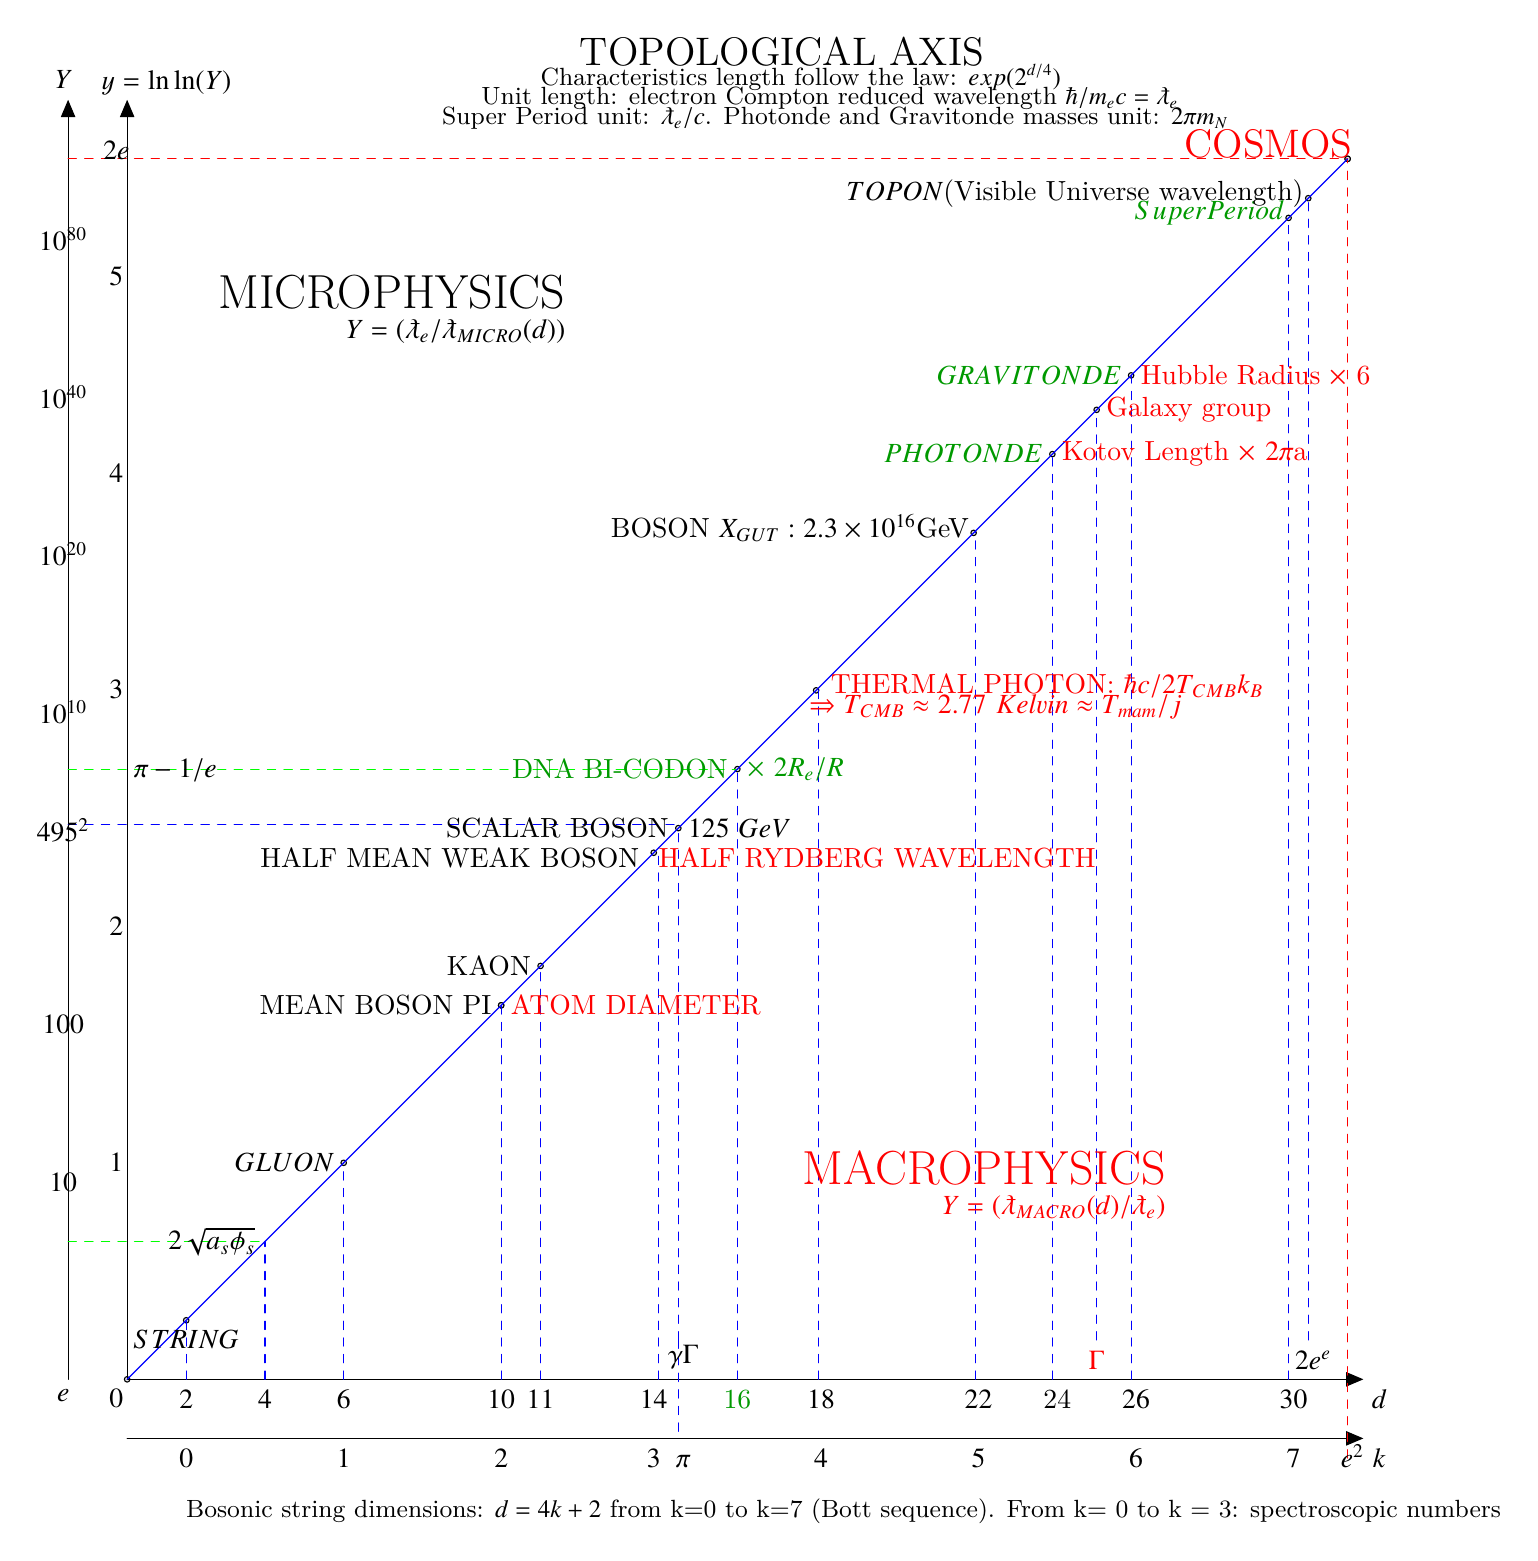
\begin{tikzpicture}[line cap=round,line join=round,>=triangle 
45,x=0.25cm,y=0.25cm]

\tkzDefPoint(-31.0,-31.0){A} %\tkzDefPoint(5.,3.43){B} \tkzDefPoint(5.,0.){C} \tkzDefPoint(31.0,31.0){Y}
\tkzDefPoint(-28.0,-28.0){B}
\tkzDefPoint(-20.0,-20.0){C}
\tkzDefPoint(-12.0,-12.0){D}
\tkzDefPoint(-12.0,-12.0){E}
\tkzDefPoint(28.0,28.0){F}
\tkzDefPoint(-4.25,-4.25){G}
\tkzDefPoint(4.0,4.0){H}
\tkzDefPoint(12.0,12.0){I}
\tkzDefPoint(-3.0,-3.0){J}
\tkzDefPoint(16.0,16.0){K}
\tkzDefPoint(18.25,18.25){L}
\tkzDefPoint(20.0,20.0){M}
\tkzDefPoint(29.0,29.0){N}
\tkzDefPoint(-10.0,-10.0){P}
\tkzDefPoint[color=red](31.0,31.0){Q}
\tkzDefPoint(31.0,31.0){Y}
\tkzDrawPoints(A,B,C,D,F,E,G,H,I,J,K,L,M,N,P,Q,Y)
%\tkzMarkRightAngle(A,D,C)
%\tkzLabelPoints[text=red,right](G,H)
%\tkzMarkAngle[fill=blue!40,size=1.4cm,opacity=.5](C,A,B)
%\tkzLabelAngle[pos=1.6](C,A,B){$\theta$}
\tkzDefMidPoint(A,Y) \tkzGetPoint{BI-CODON}
\coordinate (center) at (BI-CODON);
%\tkzLabelPoints[below,color=green](BICODON)
\tkzDrawPoints(BI-CODON)
\draw [->] (-31.0,-31.0) node[left]{} -- (-31.,34.) node[right]{}; % scale Y
%\draw [->] (31.0,-31.0) node[left]{} -- (31.,31.) node[right]{}; % 
\draw [->] (-31.0,-31.0) node[left]{} -- (31.8,-31.0) node[right]{}; % scale d
\draw [->] (-31.0,-34.) node[left]{} -- (31.8,-34.) node[right]{};   % scale k
\draw [->] (-34.0,-31.) node[left]{} -- (-34.,34.) node[right]{};   % scale Y'
%%% Blue Dashed Horizontal lines
\draw [-,color=green,dashed] (-34.0,-24.) node[left]{} -- (-24.,-24.) node[right]{};   % \sqrt{a_s} horizontal line
\draw [-,color=blue,dashed] (-34.0,-2.8) node[left]{} -- (-2.8,-2.8) node[right]{};   % Scalar Boson horizontal line
\draw [-,color=green,dashed] (-34.0,0.) node[left]{} -- (0.,0.) node[right]{};   % bicodon horizontal line
\draw [-,color=red,dashed] (-34.0,31.) node[left]{} -- (31.,31.) node[right]{};   % Cosmos horizontal line
%%% Blue Dashed Vertical lines
\draw [-,color=blue,dashed] (-28.0,-31.) node[left]{} -- (-28.,-28.) node[right]{};   % String vertical line
\draw [-,color=blue,dashed] (-24.0,-31.) node[left]{} -- (-24.,-24.) node[right]{};   % \sqrt{a_s} vertical line
\draw [-,color=blue,dashed] (-20.0,-31.) node[left]{} -- (-20.,-20.) node[right]{};   % Gluon vertical line
\draw [-,color=blue,dashed] (-12.0,-31.) node[left]{} -- (-12.,-12.) node[right]{};   % ATOM DIAMETER vertical line
\draw [-,color=blue,dashed] (-10.0,-31.) node[left]{} -- (-10.,-10.) node[right]{};   % Kaon vertical line
\draw [-,color=blue,dashed] (-4.0,-31.) node[left]{} -- (-4.,-4.) node[right]{};   % Half Mean Weak Boson vertical line
\draw [-,color=blue,dashed] (-3.0,-29.) node[left]{} -- (-3.,-3.) node[right]{};   % Scalar Boson vertical line
\draw [-,color=blue,dashed] (-3.0,-29.) node[left]{} -- (-3.,-34.) node[right]{};   % \gamma\Gamma->\pi vertical line
\draw [-,color=blue,dashed] (0.,-31.) node[left]{} -- (0.,0.) node[right]{};   % Bicodon vertical line
\draw [-,color=blue,dashed] (4.1,-31.) node[left]{} -- (4.1,4.1) node[right]{};   % Thermal Photon vertical line
\draw [-,color=blue,dashed] (12.1,-31.) node[left]{} -- (12.1,12.1) node[right]{};   % Boson X GUT vertical line
\draw [-,color=blue,dashed] (16.,-31.) node[left]{} -- (16.,16.) node[right]{};   % Photon vertical line
\draw [-,color=blue,dashed] (18.25,-29.) node[left]{} -- (18.25,18.25) node[right]{};   % Galaxy group vertical line
\draw [-,color=blue,dashed] (20.0,-31.) node[left]{} -- (20.0,20.) node[right]{};   % Gravitonde vertical line
\draw [-,color=blue,dashed] (28.0,-31.) node[left]{} -- (28.0,28.0) node[right]{};   % Super Period vertical line
\draw [-,color=blue,dashed] (29.,-29.) node[left]{} -- (29.,29.0) node[right]{};   % Topon vertical line
\draw [-,color=red,dashed] (31.0,-35.) node[left]{} -- (31.,31.) node[right]{};   % Cosmos vertical line

\draw[color=blue] (A) -- (Y);
\node [anchor = text=blue] at (-8.,35.75) {\Large{TOPOLOGICAL AXIS}};
\node [anchor = text=black] at (-10.,34.75) {\small{Characteristics length follow the law: $exp(2^{d/4})$}};
\node [anchor = text=black] at (-13.,33.75) {\small{Unit length: electron Compton reduced wavelength $\hbar /m_e c=\lambdabar_e$}};
\node [anchor = text=black] at (-15.,32.75) {\small{Super Period unit: $\lambdabar_e/c$. Photonde and Gravitonde masses unit: $2\pi m_N$}};
\node [anchor = text=black] at (-28.,-38.0) {\small{Bosonic string dimensions: $d=4k+2$ from k=0 to k=7 (Bott sequence). From k= 0 to k = 3: spectroscopic numbers}};
\node [anchor = east,text=red] at (31.75,31.75) {\Large{COSMOS}};
\node [anchor = south] at (-28.,-33.0) {$2$};
\node [anchor = south] at (-28.,-36.0) {$0$};
\node [anchor = north] at (-28.,-28.0) {$STRING$};

\node [anchor = south] at (-24.,-33.0) {$4$};
\node [anchor = east] at (-24.,-24.0) {$2\sqrt{a_s\phi_s}$};
\node [anchor = south] at (-20.,-33.0) {$6$};
\node [anchor = south] at (-20.,-36.0) {$1$};
\node [anchor = east] at (-20.,-20.0) {$GLUON$};
\node [anchor = south] at (-12.,-33.0) {$10$};
\node [anchor = south] at (-10.,-33.0) {$11$};
\node [anchor = south] at (-12.,-36.0) {$2$};
\node [anchor = east] at (-12.,-12.) {MEAN BOSON PI};
\node [anchor = west,color=red] at (-12.,-12.) {ATOM DIAMETER};
\node [anchor = east] at (-10.,-10.) {KAON};
\node [anchor = south] at (-4.25,-33.0) {$14$};
\node [anchor = south] at (-4.25,-36.0) {$3$};
\node [anchor = east] at (-4.5,-4.5) {HALF MEAN WEAK BOSON};
\node [anchor = west,color=red] at (-4.5,-4.5){HALF RYDBERG WAVELENGTH};
\node [anchor = south] at (-2.75,-31.0) {$\gamma\Gamma$};
\node [anchor = south] at (-2.75,-36.0) {$\pi$};
\node [anchor = east,color=black] at (-3.0,-3.0){SCALAR BOSON};
\node [anchor = west,color=black] at (-3.0,-3.0){$125~GeV$};
\node [anchor = south,color=black!40!green] at (0.,-33.0) {\textbf{16}};
\node [anchor = east,color=black!40!green] at (0.,0.0) {DNA BI-CODON};
\node [anchor = west,color=black!40!green] at (0.,0.0) {$\times~2R_e/R $};
%\node [anchor = west,color=black!40!green] at (0.,0.0) {$\times$ $2R_e/R\approx \mu^3\approx (\tau/\sqrt{e/2})^2$};
\node [anchor = south] at (4.25,-33.0) {$18$};
\node [anchor = south] at (4.25,-36.0) {$4$};
\node [cross,anchor = west,color=red] at (4.25,4.25){THERMAL PHOTON: $\hbar c/2T_{CMB}k_B$};
\node [cross,anchor = west,color=red] at (3.15,3.15){$\Rightarrow T_{CMB} \approx 2.77 ~Kelvin \approx T_{mam}/j$};
\node [anchor = south] at (12.25,-33.0) {$22$};
\node [anchor = south] at (12.25,-36.0) {$5$};
\node [anchor = east,color=black] at (12.25,12.250){BOSON $X_{GUT}:2.3 \times 10^{16}$GeV};
\node [anchor = east,color=black!40!green] at (16.,16.){$PHOTONDE$};
\node [anchor = west,color=red] at (16.,16.){Kotov Length $\times$ $2\pi$a};
\node [anchor = west,color=red] at (18.25,18.250){Galaxy group};
\node [anchor = south,color=red] at (18.25,-31.0) {$\Gamma$};
\node [anchor = east,color=black!40!green] at (20.,20.0){$GRAVITONDE$};
\node [anchor = west,color=red] at (20.,20.0){Hubble Radius $\times$ 6};
\node [anchor = south] at (16.25,-33.0) {\textbf{24}};
\node [anchor = east,color=black!40!green] at (28.25,28.250){$Super Period$};
\node [anchor = east,color=black] at (29.25,29.250){$TOPON$(Visible Universe wavelength)};
\node [anchor = east,color=black] at (-8.25,24.250){\LARGE{MICROPHYSICS}};
\node [anchor = east,color=black] at (-8.25,22.250){$Y=(\lambdabar_e/\lambdabar_{MICRO}(d))$};
\node [anchor = east,color=red] at (22.25,-20.250){\LARGE{MACROPHYSICS}};
\node [anchor = east,color=red] at (22.25,-22.250){$Y=(\lambdabar_{MACRO}(d)/\lambdabar_{e})$};
\node [anchor = south] at (20.25,-33.0) {$26$};
\node [anchor = south] at (20.25,-36.0) {$6$};
\node [anchor = south] at (28.25,-33.0) {$30$};
\node [anchor = south] at (28.25,-36.0) {$7$};
\node [anchor = south] at (31.25,-36.0) {$e^2$};
\node [anchor = south] at (29.25,-31.0) {$2e^e$};
\node [anchor = south] at (32.6,-33.00) {$d$};
\node [anchor = south] at (32.6,-36.00) {$k$};
%%% Y AXIS
\node [anchor = north] at (-31.55,-31.0) {$0$};
\node [anchor = north] at (-31.55,-19.0) {$1$};
\node [anchor = north] at (-31.55,-7.0) {$2$};
\node [anchor = north] at (-31.55, 5.0) {$3$};
\node [anchor = north] at (-28.55, 1.0) {$\pi-1/e$};
\node [anchor = north] at (-31.55, 16.0) {$4$};
\node [anchor = north] at (-31.55, 26.0) {$5$};
\node [anchor = north] at (-31.55, 32.4) {$2e$};
\node [anchor = north] at (-29.0,36.0) {$y=\ln\ln(Y)$};
%%% Y' AXIS
\node [anchor = north] at (-34.25,-31.0) {$e$};
\node [anchor = north] at (-34.25,-20.0) {$10$};
\node [anchor = north] at (-34.25,-12.0) {$100$};
\node [anchor = north] at (-34.25,-2.0) {$495^2$};
\node [anchor = north] at (-34.25,4.0) {$10^{10}$};
\node [anchor = north] at (-34.25,12.0) {$10^{20}$};
\node [anchor = north] at (-34.25,20.0) {$10^{40}$};
\node [anchor = north] at (-34.25,28.0) {$10^{80}$};
\node [anchor = north] at (-34.25,36.0) {$Y$};
%% SLOPE
%\tkzLabelSegment[sloped,below,text=black](A,D){Slope $\ln(2)/4$}
\end{tikzpicture}
\caption[Graphics \ref{AxeTopologique}: Topological Axis ]{The Topological Axis follows the law $exp(2^{d/4})$ for the main physical characteristics lengths, with unit length the electron Compton reduced wavelength: $\hbar/ m_ec=\lambdabar_e$. This is the extrapolation towards smaller numbers of the Eddington's Large Number correlations, a reunion of height 2D-1D holographic relations, whose micro-macrophysics imbrication explains the double log, hence the name `Topological Axis'. The double natural logarithms $y = ln(ln(Y))$ of the main dimensionless physical quantities ($Y$) corresponds to the special string dimension series, which identifies with the spectroscopic series with spin 1/2, where $k$ is the orbital quantum number, $d = 4k + 2$, from $k = 0$ to $k = 7$, characteristics of a Bott octonion sequence, as anticipated by Atiyah, whose constant $\Gamma=\gamma a/\pi$ is central. The mean value $d=16$ connects directly with the DNA bi-codon, decisive in the Holic Cosmology, where $R_e$ is the holographic reduced Cosmos radius and $R$ the Hubble radius, whose ratio is connected with the Weinberg-Sanchez gauge couplings (Eq(4), $\phi_s$ a special value of the golden number, $m_N = a m_e$ the Nambu mass, the Kotov length $ct_{nl}$ and $j = 8\pi^2/ln2$ the scale factor \cite{Sanchez3}. In this rehabilitation of the Bosonic String Theory, the Universe appears as the final boson in the Cosmos.}

\label{AxeTopologique}

\end{table}




\begin{table}
%\label{tab:6:table6}
\caption[Table \ref{tab:6:table6}: 56 Hubble radius formulas]{56 formula for the Hubble radius $R$}
\label{tab:6:table6}
  \hskip-2.0cm\begin{tabular}{lll}
    \toprule
    %\multicolumn{3}{c}{}     \\
    \cmidrule(r){1-3}
    Formula     & Value (Gly)  & Remarks \\
    \midrule
 
 $ 2\hbar^2/Gm_em_pm_H $ & 13.81197676 & Gravitational Hydrogen Molecule radius \cite{Sanchez2}\\ 
 $ (H/p_t)~R_{1H}$ & 13.81197676 & From mono-atomic star limit radius  $R_{1H}$ \cite{Davies} \\
 $ \lambdabar_w ~(t_{nl}/t_e)^2$ & 13.81197676 & Identification predicting $t_{nl}\approx 9600.591457 s$~(Eq.(5)) \\
 $ (\lambdabar_{p} \lambdabar_{H})^{1/2} ~(WZ)^4$  & 13.81197676 & Symetrising the published relation $a_G \approx W^8$ \cite{Rees} \\
 $\lambdabar_{e} ~2^{128}/d_e^2(m_H/m_p)^6$  & 13.81197676   & Empirical, from the Combinatorial Hierarchy Lucas Large Number \cite{Bastin}\\
  $(n_tp_W/1836p)^{1/2}\lambdabar_{e} (2^{18}/\pi \sqrt a)^{10}$  & 13.811977   & From $(2g_3)^{21} \approx s_{65}/2\pi$; $p_W = 6\pi^5$ and $s_{65} \approx (2\pi)^2 \sqrt a$\\
  $ (1/g_0) ~\lambdabar_H ~(R_C/2^{128}l_P)^{1/2} $  & 13.811978 & From $1/g_0 = 1+g_1^2+g_2^2\approx2a^3/pp_G$, with $p_G = P/2^{127/2}$\\ 
 $ (\lambdabar_{p} \lambdabar_{H})^{1/2}~ a_w^{7/2}~ a/2\sqrt 5 $  & 13.811978 & From $(WZ)^8 \approx a^2a_w^7/20$\\
 $ \lambdabar_e ~(p_{hol}/p)^2~ e_3 ^{\sqrt a/2}$ & 13.81198 & Liaison between $e_3 = exp(exp(e))$ and $p_{hol}^2 = 4a^3/3$   \\
 $ (32 \beta^2 /\pi^3) ~\lambdabar_{CMB}^3/ \lambdabar_Z^2$ & 13.81200 & from the holographic relation $2\pi R/\lambdabar_e \approx (4\pi/3) (\lambdabar_{CMB}/\lambdabar_{H_2})^3$ \cite{Sanchez2}\\  
 $(H/p_W)~(2\pi^2 a^3)^5~ \lambdabar_{e} $ & 13.81196 & with $p_W = 6\pi^5$, 5D holography in the gravitational Hydrogen molecule \cite{Sanchez3}  \\
  $\lambda_{p} ~(pH)^{3a_s/4}  $ & 13.81193 & confirms the strong coupling $a_s$  \\
  $ 4 ~a^4 ~\lambdabar_{e} ~(m_{bc}^{(0)}/m_H)^9 (p_t/p_W)^2  $ & 13.81196 & DNA bi-codon mass as calculation basis  \\
  $ \lambdabar_{e}~ (WH/Zp)^{1/2}~C_y^{(0)32}/6f(26)   $ & 13.81195 & Cytosine topologic pertinence  $C_y^{(0)} \approx f(10)= f(26)^{1/16} $  \\
  $ \lambdabar_{e}~ (N_{ph}  ~(n_t/p_t)^2/\pi \sqrt{g_0})^{1/7} $ & 13.81197 & with $N_{ph}$ the Cosmos photon number, confirms that the Universe is a cosmic boson \\
 $R_C ~(a_se^{2/a}210^{-210})^{1/8}$  & 13.81198    & With the holic number $210^{210}$, confirming the couple Universe- Cosmos \\
 $ l_{P} ~\sqrt a ~(\mu^{\mu}~Wp/ZH)^{1/8}$  & 13.81198 & Shows the pertinence of the computational term $\mu^{\mu}$   \\
  $(H/p_t)~(ad_e/137)^4 ~R_{R_c,M_N} $ & 13.81203    & From the geo-adimensional Cosmos-Universe (Fig.1)\\
 $(137\beta/a)^2~R_c~R_e~l_P^2/a_w l_{nl}^2\lambdabar_{bc}^{(0)}$ & 13.81194    &  Holic Principle, with the reduced wavelength of the DNA bi-codon. \\
$(\pi ~a/6\times 137) ~\lambdabar_e ~(1/g_0)^{210} $ & 13.81185 & From $(1/g_0) \approx 2R/R_e \approx (R/\lambdabar_e)^{1/210}$ (Eq. (14)) \\   
 $ (136/137)~2~l_{nl}~a^3~f(16)$  & 13.8120    & Empirical, with the central value $f(16) = e^{16}$ \\ 
  $ (137^4/ap_t^2)~\lambda_{WCMB}~(e^a/4\pi)^{1/2}$  & 13.8120    & Confirming the Wien CMB wavelength, from $4\pi (R_e/\lambda_{WCMB})^2 \approx e^{a}$ \\  
$ \lambdabar_{e} ~ (1/q)^{3\pi a_s}/496$  & 13.8124    & Confirms the strong coupling $a_s$ and the electric charge $q$ \\ 
 $(\lambdabar_{p}~ \lambdabar_{H})^{1/2} ~a_w^4~ a^{14}/137^{16}$  & 13.8119    &  $137,a,a_w$ as computation basis \\
  $(2a/137)~q^2 ~Z^{16} \lambdabar_{p} \lambdabar_{H}/2^{127}\lambdabar_{e} $  & 13.8221    & Cosmic role of electric charge $q = g_1 \cos \theta = g_2 \sin \theta$  \\
 $4~o_2~\sqrt Z~ \lambdabar_{e}\lambda_{CMB}/l_P     $  & 13.8129    &Confirms the cosmic thermal bath and the couple GC with mass $o_2 m_H$    \\
 $ (H/p_t)~(Gm_n/c^2) ~(10N_{Ed}/3)$ & 13.8125 & From the Eddington Number $136 \times 2^{256}$ and the gravitational parameter 10/3 \cite{Sanchez3}  \\
 $ R_e ~({f(-2)}/exp(exp(-g_1))^{128}/d_e^3$  & 13.8117    & Symmetry $R_e/R$ associated to symmetry f(2)-$g_1$  (string-SU(1) gauge coupling)     \\
 $ 2~\lambdabar_{e} ~((1836+s_{65})/2)^{\sqrt a} $  & 13.8123 & Pertinence of the symmetry 1836-1848 (Eq.(25))\\
  $ (\lambdabar_{p}~ \lambdabar_{H})^{1/2} ~(P/a^{13/2})^5/2\sqrt 5 $  & 13.8124 & From the relation $a_w^7 \approx P^{3+7}/a^{(7 + 127)/2}$ \cite{Sanchez3}\\
  $6~(\lambdabar_{e}^2/\lambdabar_w)~(a/\pi)^{16}$  & 13.8124    & From the Topologial Axis: $f(18)\approx H^3 \approx (a/\pi)^4 (6^{1/2}a_w)^{1/2}$  \\
  $   (1/q)^{3\pi a_s}~\lambdabar_{e}/496$  & 13.8124    & Confirms the strong coupling $a_s$ and the electric charge $q$  \\ 
  $4~\lambdabar_e~a~ W~Z~ F ~ (p_tH)^3$  & 13.817    & Shows a symmetry $a~ W~Z~ F$ \\
  $4~l_{nl}~ (p_t~H/d_e)^2$  & 13.815    & Confirms the non-local Kotov length \\
 $\lambdabar_e ~(2/d_e^8)^{128}/(2g_0-1)$  & 13.815    &  From the Combinatorial Hierarchy Lucas Large Number [12] \\ 
  $ 2~\lambdabar_{H}2^{210} ~(a_w/P)^2  $ & 13.811 & Pertinence of the holic term $2^{210}$ \\
  $ \lambdabar_e ~e^a/p_t^6\Gamma$ & 13.811 & confirms the pertinence of the Atiyah constant $\Gamma$  \\
  $ l_{P} ~(\pi 210^{210}/8)^{1/8}$  & 13.81    & Pertinence of the holic term $210^{210}$  \\
 $R_e~ a^a/\Pi_{heur}$  & 13.81    & with the product of the 20 happy sporadic groups $\Pi_{heur}\approx e^{674.5210287}$  \\
$ 2~\hbar^2/Gm_em_pm_n $ & 13.80 & \underline{c-free dimensional analysis} \cite{Sanchez4}  \\
 $(\Pi_+/\Pi_0) \lambdabar_{e}~ e^{1/(g_0-g_2)}$ & 13.82 & Confirms the pertinence of $g_0$ and $g_2$  \\
 $l_{nl}~2~p_t^3~H/d_e $ & 13.82 & $p$ and $H$ as computation basis  \\
 $ (\lambda_{CMB}/(j+1))^2/l_P$ & 13.80 & Central role of mammal temperature: $T_{mam}\approx j T_{CMB}$, with $j = 8\pi^2/ln2$ \\
  $ 2~ \lambdabar_{e}~ (1/sin\theta)^{10d_e\sqrt {137}} $ & 13.80 & Corresponds to $(1/sin\theta) \approx 3/\sqrt2 \approx p^{1/10}$   \\
  $ \lambdabar_{e} ~\pi^{155/2}$ & 13.80 & $\pi$ calculation basis: $2^{1/155} \approx \pi^{1/16^2}  \approx (2\pi)^{1/3\times 137} $  \\
  $ 2~\lambdabar_{e}~ e_3^{2\sqrt a_s}$ & 13.79 & Pertinence of the basic economic number $e_3 = e^{e^e}$  \\
  $ \lambdabar_{e} ~(6/\pi)^{r_H/\lambdabar_e}$ & 13.78 & $6/\pi$ calculation basis   \\  
$ \lambdabar_{e} ~\Gamma^{55/2}$ & 13.77 & Atiyah's constant $\Gamma$ calculation basis   \\  
 $ g(6) ~\lambdabar_{e} $ & 13.82 & \underline{with the reduced topological function} $g(k) = exp(2^{k+1/2})/k$, for k = 6, d = 26  \\
 $ 2~l_{nl}~(a\mu)^3 $ & 13.84 & Confirms the non-local Kotov length \\
 $ (2l_{nl}^3/r_e)^{1/2}$  & 13.75    & 2D-3D Holography with the non-local length $l_{nl}$ \\
  $ (r_e^2R_C)^{2/3}/l_{nl}$  & 13.75    & Confirms the Cosmos non-locality \\
 $ (2~\lambdabar_{e}/3) ~(\lambdabar_{CMB}/\lambdabar_{H_2})^2$ & 13.90 &  2D-3D holography in the hydrogen molecule \\   
   $ (4~\pi ~\lambda_{CMB})^4/r_H^3$ & 13.78 & Confirms the CMB invariance \\ 
    $ (l_P/2)~(\lambdabar_{CMB}^2\lambdabar_p/\lambdabar_{CNB}r_e^2)^6$  & 13.7    & Complementarity of photons and neutrinos backgrounds \\
 
 %\bottomrule
  \end{tabular}
\end{table} 
 

\subsection{The Classical Universe Radius and the Cosmic Gravity-CMB-Microphysics connection}
The standard theory associates conservation law with symmetry. However, a conservation law can be seen as the result of a computation. Considering that the Universe is a computing black-hole of radius $R$, this introduces the length $(Rl_P^2)^{1/3} \approx 10^{-15} $ m \cite{Sanchez5}. The identification with the \textit{invariant} electron classical radius defines the Classical Universe Radius $R_e$. \textit{It is the radius eliminating $c$ between the classical electron radius and the Planck length formula. This radius presents a very precise dramatic holographic property involving the CMB Wien wavelength}:

\begin{equation}
 \left\{
    \begin{array}{ll}
    R_e = 2r_e^3/l_P^2 = 2 \hbar^2/Gm_N^3 ~~~~~~~~~~~~ M_N = m_P^4/m_N^3 \\
   4\pi(R_e/\lambda_{WCMB})^2 \approx e^a
    \end{array}
\right.
\end{equation}

    
where $M_N = R_ec^2/2G $ is the associated critical mass, implying the Nambu mass $m_N = am_e$, central in particle physics \cite{Nambu}. The OCP introduces the "Weinberg-Sanchez" natural geometric extension of the Weinberg triangle \cite{Taylor}, $1/g_0 = 1+g_1^2 +g_2^2 = 1 + (Z/H^{(0)})^2$. With the BE-Higgs scalar boson mass ratio, by respect to electron:  $H^{(0)} = 495^2$ (125.208 GeV)\cite{Sanchez2}, the radius ratio $R_e/R$ obeys the following $10^{-7}$ precise relations, involving $G$ through $p_G = P/2^{127/2}$ (from the Combinatorial Hierarchy \cite{Bastin}) and the Wien factor $w_i$. From the OCP, the following coupling $g_3$ and the electric charge $q$ are proposed: 
\begin{equation}
 \left\{
    \begin{array}{ll}
    1/g_0 = 1+g_1^2 +g_2^2 \approx 2R/R_e \approx 2(H/p_t)(\beta \sqrt {a_s}/w_i)^{1/2}\\
   tg \theta =  g_1/g_2 = g_0/g_3\\
   g_1 cos \theta = g_2 sin \theta = (4\pi_q/a)^{1/2} \approx y\Pi_+/2d_e\sqrt F  ~~~~~;~~~~~  3^{11-1}\approx 6(2\pi_q)^5 \approx \pi a^2   
    \end{array}
\right.
\end{equation}

Note that the electric charge is tied to the Mirimanoff prime 11 \cite{Mirimanoff}, showing the connection supersymetry-supergravity 10 = 11 - 1. The small difference between $g_0$ and $g_2$ induces formula in the Hubble and Cosmos Tables. In this manner, the gauge couplings are connected with the  Wien factor $w_i$, whose pertinence is not reckognized in the present standard model. Moreover, there is a direct confirmation, precise to 0.1 ppm, of the CMB temperature invariance:
\begin{equation}
K_n = (32 \xi(3) /3\pi)^{1/2} R l_P/(\lambdabar_{CMB}^3 \lambdabar_H)^{1/2} \approx K_E (1-1/12^2)^{-1/2} 
 \end{equation}

\textit{This means there is a symmetry between radiation and matter, totally unexpected in the present standard theory. This relation has the same form than that of Eddington : $\sqrt{M/m_e} = R/2\lambdabar_H$, equivalent to Eq. (5)}.
%1/g_0 = 1+g_1^2 +g_2^2 = 1 + (Z/H^{(0)})^2 \approx (R_e/2R) (p_G/H) = g_2/g_1g_3 \approx 2(H/p_t)(\beta sqrt a_s/w_i)^{1/2}
 %\end{equation}

\subsection{The Tachyonic Holographic Cosmos}

The radius $R_e$, about 30\% larger than $R$, was identifed to the holographic reduced Cosmos radius \cite{Sanchez3}, defined by the Bekenstein-Hawking entropy of the $R_e$-radius sphere \cite{Bekenstein}: $\pi (R_e/l_P)^2 = 2\pi R_C/l_P$, so:   

 \begin{equation}
R_c = R_e^2/2l_P \approx 2^{128} l_P (Rg_0/ \lambdabar_H)^2 \approx 9.075773 \times 10^{86} m 
 \end{equation}
 
 \textit{The Table \ref{CosmosTable} presents 54 simple formula confirming this Cosmos radius $R_c$.} In particular, there is the dramatic geometrical property, the "Geo-adimensional Cosmos-Universe couple" (Fig.1): 

\begin{equation}
(ln(R_c/\lambdabar_e))^2 \approx (ln(M_N/m_e)^2 + 2(ln(R/\lambdabar_e))^2
\end{equation}

where the 2 factor comes from \textit{the local character of the speed $c$} \cite{Sanchez2}. 



\begin{table}
\caption[Table \ref{CosmosTable}: 55 Cosmos radius formula]{55 formula for the Cosmos radius $R_C$}
\label{CosmosTable}
  \hskip-2.0cm\begin{tabular}{lll}
    \toprule
   % \multicolumn{3}{c}{}                   \\
    \cmidrule(r){1-3}
    Formula     & Value ($10^{86}$m)  & Remarks \\
   \midrule
 
 $ R_e^2/2l_P $ & 9.07577 & 1D-2D Holographic Principle with $R_e$ \cite{Sanchez2}   \\
 $ \lambdabar_e ~ exp(exp(exp(exp(exp(-g_2)))))  $ & 9.07577 & The final log of $R_c/\lambdabar_e$ is a SU(2) coupling: $g_2 \approx W/(495^2+(\tau/\mu)^2)$  \\
 $ (\lambdabar_{W}\lambdabar_{Z})^{1/2}e^{1/(a-9)} ~ exp(exp(exp(exp(exp(-g_0)))))  $ & 9.07579 & from the connections $g_0 \approx g_2$ and $a - 9 \approx 2^7$ \\
 $ e^{210}~ R ~(f(16) e^{e^6} 9\mu/n_t)^{-1/6}  $ & 9.07577 & confirms the role of the central topologic term $f(16) = e^{16}$   \\
 $e^{210}~l_{Wien}\beta (\sin \theta_{1})^4$ & 9.07577 & confirms the Holic Principle and the CMB temperature invariance  \\
 $ 2^{128}~ l_P (g_0R/\lambdabar_H)^2 $ & 9.07577 & confirms $1/g_0 = 1+g_1^2 +g_2^2 = 1 + (Z/H^{(0)})^2$  \\
 $ R~p_t (6d_e P^{\sqrt a - 4}/\pi)^{1/3}$ & 9.07574 & from the cosmic atomic mass $M_c/m_H \approx P^{\sqrt a}$  \\
 $ l_P (R_C/\lambdabar_{e}^{g_3}~  (p_G/2a)^{1/2}$ & 9.07574 & confirms the SU(3) coupling $g_3$  \\
  $ \lambdabar_{e} ~(a^{3/2}/1837) y^{64a_s}$ & 9.07579 & from $y^{a_s} \approx 3^4 - 1$ \\
 $ \lambdabar_{e} ~14 p_t^2/p_Wn_t (a/4)^{64}$ & 9.07579 & empirical, with $p_W = 6\pi^5$ \\
 $ 2\lambdabar_{e}~ (sin_Z \theta_{eff})^{-4} (4a_s)^{64}$ & 9.07777 & empirical, implying a relation between $a$ and $a_s$ \\
 $ l_P ~(\Pi_+/18)3^{256}$ & 9.07586 & confirms the cosmic base 3 \\
  $ R ~ a^6 ~(12^{32}/P)^{4} 1839/4H$ & 9.07587 & base 12 \\
  $\lambdabar_{e} ~ (n_t/a^2g_0) ~(3)^{210} $ & 9.07567 & base 3 \\
 $ g_2\lambdabar_{e}~(60H/61p_t) ~(1/q)^{2^6} $ & 9.07548 & confirms the electric charge $q$;  $61/60 \approx (n_t/p_t)^{12}$  \\
 $ l_P ~(2/\sqrt5)(80)^{64}$ & 9.07510 & implies the musical property (16 ppb): $((3/2)^4/5)^{256} \approx 24 (a/137)^{32}(p_t/p_W)^{1/2}$ \\
 $ e^{\mu} ~\lambdabar_{CMB} (R_e/R)^2 (p_t/p_{t0})^4$ & 9.07584 & confirms the CMB temperature invariance, with $p_{t0}$ = 1836 \\
 $ e^{\mu} ~\lambda_{Wien} e/2\beta^2 \sqrt d_e$ & 9.07575 & confirms the CMB temperature invariance, through the Wien wavelength\\
 $ e^{\mu} ~l_{phCMB} ~((a-136)p_t/p_{t0})^2$ & 9.07573 & confirms the CMB temperature invariance, through its photon length $l_{phCMB}$\\
 $ e^{\mu}~ \lambdabar_{e}~ \beta^{1/2} (p_t/n_t)^{1/4} $ & 9.07576 & confirms the CMB temperature invariance \\
$ 2(a/137\beta)^2 ~l_{nl}^4 ~\lambdabar_{bc}^{(0)}/R_e \lambdabar_el_P^2 $ & 9.07580 & Holic Principle, with the reduced wavelength of the DNA bi-codon \\
 $ l_P ~ (\sqrt{a_w}(a)^2)^{16}  $ & 9.07568 & bases  $a_w$ and $a_s$, the nuclear couplings  \\
 $ l_P ~ \sqrt{1 + (sin\theta_1)^2}~a^{j/2}  $ & 9.07566 & base $a$ the electric coupling, with $j$ the scale factor \cite{Sanchez2} \\
 $ l_P ~ (210^{210}(8e)^{-1/2})^{1/4}  $ & 9.07585 & Holic central term $210^{210}$  \\
 $ l_P ~ \sqrt2 ~ (p_t/n_t)^6 e^{280}  $ & 9.0767 & base e  \\
 $ l_P ~ (Zd_e/W) ~7^{12^2}  $ & 9.075 & base 7  \\
 $ \lambdabar_e ~ 6^{128}/(1+1/\sqrt 2)  $ & 9.075 & base 6 ; $6/(1+1/\sqrt 2) \approx \mu d_e^2/\sqrt \tau$\\
 $ \lambdabar_e ~ e^{1/2a} 6^{p_G/\sqrt a}  $ & 9.076 & base 6 \\
 $ 2r_H~ 3^{210}/1830$& 9.076 & base 3 Holic term, with $ 1830 = (60\times 61)/2 $   \\
  $ \lambdabar_e ~ (1+1/\sqrt 2)^{6a_s^2+1}  $ & 9.085 & base $1+1/\sqrt 2$ \\
  $ \lambdabar_e ~ 5^{2a_s^2+1}/6  $ & 9.082 & base 5 \\
  $ l_P ~ (7/6)^{(1836p)^{1/2}}/2e^2  $ & 9.085 & base $7/6 \approx a^{1/32}$ \\
   $ \lambdabar_e ~ ((1/q)^{a}~W/aF)^2  $ & 9.082 & base $1/q$ \\
 $  l_P~ e^{s_{65}n_tq/2p_W}$& 9.077 & confirms the terminal Euler number $s_{65} = 1848 $   \\
 $ l_P~ e^{27aq/4} ((2W+Z)/3W)^2(n_t/p_t)^2$& 9.076 & confirms the charge $q$   \\
  $l_P~(p/H) ~(R \Pi_{26}/R_e)^{1/3} $ & 9.076 & with the product of orders of the 26 sporadic groups $e^{674.5210287}$ \cite{Sanchez2}  \\ 
   $  \lambdabar_P ~ (210^{210}/\sqrt(8e))^{1/4}$  & 9.076 & Confirm the Holic Number $210^{210}\approx \tau^{2\mu/3}\approx e^{e2\mu}$  \\
   $ \lambdabar_eg(7)~ (H/p)^2  P/6 $ & 9.076 & with the reduced topologic function for $d = 30: g(7) = f(30)/7$ \cite{Sanchez2}  \\
    $ 24 \lambdabar_e ~ \pi^{210}/a^3 $ & 9.077 & Confirms the base $\pi$ holic term \\
    $ a^2 ~\lambda_{Wien}^4/(p_Kl_P)^3 $ & 9.078 & Confirms $T_{CMB}$ with $p_K = (1+\mu +\tau)/2$ \cite{Koide} \\ 
  $  \lambdabar_e ~  ((3/4\pi)(R_1/\lambdabar_e)^7)^{1/3}   $ & 9.078 & comes from the de photons nomber, using the mono-electron radius $R_1$ \cite{Sanchez2}  \\
     $  \lambdabar_e ~ 137^{1836/(2\pi)^2}   $ & 9.078 & base 137\\
  $ \sqrt 3~l_{nl}^3/r_el_P $ & 9.07 & with the non-local length $l_{nl}$  \\
  $ \lambdabar_e~ g(7) ~(a^2p_tp_G)^2 $ & 9.08 &  \cite{Sanchez2}  \\
   $ l_P ~j^{60}~ e_3^{1/4} $ & 9.06 & base $j$, the scale factor  \\
   $ l_P ~e^{(n_t/a)^2/g_2}~(3/\pi)^{1/2} $ & 9.06 & base $e$, confirms $g_2$  \\
  $ \lambdabar_e ~e^{(p_{00}+1/2)/8} $ & 9.09 & natural base $e$, with $p_{00} = (60 \times 61)/2$ \\
  $ l_P ~(n_t^2/l_p)^{2/(sin\theta_1)^4} $ & 9.06 & bases $p_t$ and $n_t$ \\
  $ \lambdabar_e ~ $ & 9.11 & natural base $e$ in the Topological Axis\\
 $ (ln(R_c/\lambdabar_e))^2 \approx (ln(M_e/m_e)^2 + 2(ln(R/\lambdabar_e)^2) $ & 9.12 & \underline{c-observable Universe  Cosmos couple} $(R/\lambdabar_e = t/t_e)$ , fig 1   \\
  $  \l_P ~ (6/\pi)^{\pi a}  $ & 9.14 & base $6/\pi$  \\ 
 $ \lambdabar_e~ g(7) ~(\lambdabar_{CMB}/r_H)^3 $ & 9.1 & Confirms the invariance of the thermal background \cite{Sanchez2}  \\
 $  (Rl_{nl})^{3/2}/r_e^2 $ & 9.2 & From non-local holography \cite{Sanchez2}  \\
  $  l_P ~ \mu^{\mu R_e/3R}  $ & 9.0 & $\mu$ calculation basis, close to holic base $210$   \\
 
 %\bottomrule
  \end{tabular}
\end{table} 
        
     
\subsection{The Non-Local Period: the Photon and Graviton masses}
The Topological Axis rehabilitates the bosonic part of the string theory which has the apparent imperfection it includes tachyons. In fact, it is rather an advantage in order to explain the quasar non-Doppler oscillation, introducing a non-local period $t_{nl} \approx 9600,06 (2) $ s \cite{Kotov}. Indeed, the ratio of this period and the electron period $t_e = h/m_ec^2$ is precisely given by the elimination of $c$ between the electro-weak constant $a_w$ and the inverse gravitational coupling $a_G = R/\lambdabar_e $: $t_{nl} /t_e   \approx  (a_G a_w)^{1/2}$. This gives a $G$ value precise to $10^{-6}$, compatible with the BIPM $10^{-5}$ precise measurement \cite {Quinn}. This implies that the official value of $G$, \textit{the incongruous mean between incompatible measurements}, is dramatically too small by 8 $\sigma$. By analogy with the practical holography, which is a two-step process, it was introduced a two-step interaction procedure, with \textit{a precursor speed} $C = cR_C/R$ much greater than $c$, leading to the following masses for the photon and graviton \cite{Sanchez2}:

\begin{equation}
 \left\{
    \begin{array}{ll}
        m_{ph} = \hbar/c^2t_{nl}\\
        m_{gr} =m_{ph}/a_w
    \end{array}
\right.
\end{equation}

In the Topological axis, these masses correspond to the special string dimensions 24 (transverse dimensions) and 26 (main dimension), and will be determinant in the following section. Note the relation, precise to 1 ppm, between the Bohr's radius $r_H$ and the relativistic factor $1/\beta = H-p$: $f(24)^{1/26} \approx d_e (r_H/\beta\lambdabar_e)^{1/2}$, showing that the electric parameter $a = (p/H)r_H/\lambdabar_e$ is central in the Topological Axis.


 
\section{The Holic Principle}
The string theory considers space-time as a secondary property \cite{Seiberg}, so the concepts of mass, length and time are, in final, related to pure numbers. Indeed an arithmetic-physical synthesis has been anticipated by the Holic Principle  \cite{Sanchez1}, a simplified form of the Holographic Principle. 

Recall that holistic equations are prefered to differential ones, in order to eliminate free parameters. 
The systematic use of differential equations in the standard physics is the origin of the proliferation of free parameters. 

In any Diophantine equation, this Holic Principle allows to discriminate a temporal ratio $T$, acting by its square, from a spatial ratios $L$, acting by its cube (due to the 3D space). Indeed, \textit {the simplest Diophantine Equation, which implies a 2-dimensional Time}, $T^2 = L^3 = n^6$, with $n$ a natural integer, is the Diophantine form of the third law of Kepler, and implies: $L_n = r_n /r_1 = n^2$ (the Bohr's orbit law) and $T_n = t_n/t_1 = n^3$. Hence, with $v_n = r_n/t_ n$:


\begin{figure}
\centering
\includegraphics[width=5cm,height=6cm]{./figure/triaxis.png}
\caption[Figure \ref{cuboid} MLT Adimensional cuboid]{\textit{Geo-adimensional Cosmos-Universe couple}, with unit length the Electron Compton reduced wavelength. In a 3D Super-space, logarithms of physical ratios are considered vectors. The Cosmos radius $ R_C$ appears as the norm of the vector using for length and time projections the same value $R/\lambdabar_e = t/t_e$. For the mass projection it is $M_N/m_e$ where $M_N$ is the critical mass in the Cosmos \textit{reduced spherical hologram} of radius $R_e$. This is a dramatic geometrical confirmation (independent of the base for logarithms) of the Extended (2D-1D) Holographic Principle applied to the Bekenstein-Hawking Universe entropy. So the Universe is characterised by the c-equivalence $R/\lambdabar_e = t/t_e$, where $t$ is the Hubble time (no relation with any "Universe age").} 
\label{cuboid}
\end{figure} 

 \begin{equation}
 \left\{
    \begin{array}{ll}
        r_nv_n^2 = r_1v_1^2 = Gm_G \\
        r_nv_n = nr_1v_1 = n \hbar/m_{\hbar}
    \end{array}
\right.
\end{equation}

\textit{These gravito-quantum equations introduce an "hyper-symmetry" between the universal constants $G$ and $\hbar$, by respect to the mass concept: the undefined masses $m_G$ and $m_{\hbar}$}. So, this defines the conceptual trajectories:

\begin{equation}
 \left\{
    \begin{array}{ll}
        r_n = n^2 r_1 \\
        
        r_1 = \hbar^2/Gm_Gm_{\hbar}^2   
    \end{array}
\right.
\end{equation}

With $m_G = m_e^{(red)} = m_em_p/(m_e+m_p)$, the classical electron reduced mass and $m_{\hbar} = m_P/\sqrt a$, this is the Bohr's orbits distribution. The above PSHOB Cosmology includes the following 6 more special cases (Table 6), using the main masses, plus a new one: $m_{bc}$, close to $m_H^2/m_e$, \textit{which identifies with the DNA bi-codon mass}, studied in the next section.

%\begin{equation}
% \left\{
   % \begin{array}{ll}
    
   % m_G = m_e^{(red)};~~  m_{\hbar} = m_P/\sqrt a  ~~~~~~~~~~~~~ \rightarrow r_1 = r_H \\
   % m_G = m_e~~;  m_{\hbar} = m_P  ~~~~~~~~~~~~~~~~~~~~~~~~~ \rightarrow r_1 = \lambdabar_e \\
    
       % m_G = m_{\hbar} = m_N  ~~~~~~~~~~~~~~~~~~~~~~~~~~~~~~~~~ \rightarrow r_1 = R_N/2 \\
        
        
       % m_G = m_{bc} = m_{\hbar}   ~~~~~~~~~~~~~~~~~~~~~~~~~~~~~~~~ \rightarrow r_1 = 2l_{nc} \\
        
       % m_G = a^3 m_P;~~ m_{\hbar}^2 = m_pm_H ~~~~~~~~~~~~~~~~ \rightarrow r_1 = \lambda_{Wn} \\
       % m_G = m_e;~~ m_{\hbar}^2 = m_pm_H ~~~~~~~~~~~~~~~~~~~~ \rightarrow r_1 = R/2 \\
         
        % m_G = m_{bc}R_N/R;~~  m_{\hbar}^2 = m_{ph}m_{gr}    ~~~~~~~~ \rightarrow r_1 = R_C 
    %\end{array}
%\right.
%\end{equation}

%$où $R$ est le rayon de Hubble et $ R_N$ est le rayon \textit{holographique réduit} du Cosmos.

So, the PSHOB Cosmology is tied to the couple $G,\hbar$, while the classical quantum theory uses in fact the "photonde" couple $\hbar,c$, and the gravitation theory the "gravitonde" couple $G,c$. These three couples define the "Trihedra of Constants"(Fig. 2).

\textit{These neologisms 'photonde" and "gravitonde" are introduced to recall that only waves propagate, not the particles: this is a main cause of misinterpretations in quantum physics.}
 
Extrapolating the above simplest Diophantine equation with the prime numbers 5 and 7 which follow the basic prime couple 2;3, the Holic Principle proposes the exponent 5 for a mass ratio, and 7 for a field ratio (note that the lifetime of a particle depends effectively to the power 5 of its mass). So, the general resolution is:

\begin{equation}
T^2 = L^3 = M^5 = F^7 = n^{210}
 \end{equation}
 
 Note that the primes 2;3;5;7 are the terms of the two simplest solutions of the Pell-Fermat equation, which has been connected with the metric equation \cite{Sanchez1}. 
 
 Indeed, the Hubble radius "holic key" is singular, to 15 ppm, while the base 2 is confirmed to 0.3 ppm, and the base 3, to 60 ppb, in the following relations:
  
 \begin{equation}
 \left\{
    \begin{array}{ll}
        (R/\lambdabar_e)^{1/210} \approx 2R/R_e = p_G/Hg_0 \\
    \\
        (P/F)^4/p_t)^{1/210}\approx 2\\
      \\  
        ((a^2g_0/an_t) R_C/\lambdabar_e)^{1/210} \approx 3
    \end{array}
\right.
\end{equation}

with $p_t$ the proton-electron mass ratio and $n_t$ the neutron-electron mass ratio. Note that 3 is the optimal integer base, the closest integer to $e$ \cite{Hayes}. This is tied to the economic functional definition of $e$, whose square interconnects the main musical ratios, using the primes 2;3;5, while \textit{the ratio 7/6, unknown in classical music, connects with $a$}. Recall that, according to Euler "music is an inconscious calculation":

\begin{equation}
 \left\{  
    \begin{array}{ll}
       x^{1/x} ~~maximal~~ for~~ x = e\\
       \\
        e^2\approx (3/2)^5 \approx (4/3)^7\approx (5/4)^9\approx (6/5)^{11}\approx (7/6)^{13} \approx a^{13/32} \approx \mu^{3/16}\\

    \end{array}
\right.
\end{equation}

\textit{So the base 7 is also pertinent. It is foreseen that special music could use also the base 7. A symmetric use of these four bases 2;3;5;7 explains the above role of the global base 210, so justifies the brute muon mass. }

 

 
\begin{table}
\caption[Table \ref{tab:5:table5}: PSHOB Cosmology.]{PSHOB cosmology (Eq.(12))}
\label{tab:5:table5}
  \hskip-2.0cm\begin{tabular}{lllll}
    \toprule
    %\multicolumn{4}{c}{}                   \\
    \cmidrule(r){1-4}
    $m_G$ & $m_{\hbar}$    & $r_1 = \hbar^2/Gm_G m_{\hbar}^2$  & Precision &Arithmetic Property \\
    \midrule
    
    $m_e$ & $m_P $ & $\lambdabar_e$: Electron reduced wavelength   & exact & \\
    $m_e^{(red)}$ & $m_P/\sqrt a $ & $r_H$: Bohr's radius   & exact & $ r_H/\lambdabar_e \approx 137 = 2^7+2^3+2^0 $\\
    $m_N $ & $m_N$   & $R_e/2$: half cosmos reduced holographic radius  &  exact & $R_e/\lambdabar_e \approx (3^3)^{3^3}$ \\
    $m_{bc}^{(0)} $ & $m_{bc}^{(0)}$   & $2l_{cc}$: double non-local length & $-6.3 \times 10^{-3}$ & $ l_{cc}/\lambdabar_e \approx \pi^{50}$  \\
    $m_Pa^3 $ & $\sqrt {m_pm_H}$  &$\lambda_{Wn}$: Wien CMB wavelength (thermal background) & $-3.2 \times 10^{-4}$ &$\lambda_{Wn}/l_P \approx \pi^{64}$\\
    $m_e $ & $\sqrt {m_pm_H}$   & $R/2$: half Universe radius &exact& $R/\lambdabar_e \approx g(6) \approx 2^{2^7}\approx (2R/R_e)^{210}$   \\
    $m_{bc}^{(0)}R_e/R $ & $\sqrt{ m_{ph}m_{gr}}$   & $R_C$: Cosmos radius = $RC/c = (R/2)m_N^3/m_{bc}m_{ph}m_{gr}$ & $4.7 \times 10^{-4} $& $ R_C/\lambdabar_e \approx e^{e^{2e}} \approx 6^{2^7}\approx (2R/R_e)^{64a_s}  $\\
    
  
         
   \bottomrule
  \end{tabular}
\end{table}







\begin{figure}
\label{figure2}
\centering
\begin{tikzpicture}[scale=2, tdplot_main_coords,axis/.style={->,dashed},thick]
%\tkzDefPoint(1.,-1.,0.75){A} \tkzDefPoint(4.9,0.,-0.75){B} \tkzDefPoint(3.12,0.,-1.74){C}
%\draw[step=1cm,gray,very thin] (-4,-4) grid (4,4);
\node[shape=circle,draw,fill=black,inner sep=1pt] (O) at (0,0,0){};
%\node[shape=circle,draw,fill=black,inner sep=1pt] (M) at (1,-1,0){};
\draw[axis] (0, 0, 0) -- (3, 0, 0) node [right] {$G$};
\draw[axis] (0, 0, 0) -- (0, 2, 0.25) node [above] {$\hbar$};
\draw[axis] (0, 0, 0) -- (0, 0, 1) node [above] {$c$};
\coordinate  (d1) at (1,0,1){};
%\coordinate  (d2) at (3,-2,-1){};
\coordinate  (M) at (1,-1,0){};
%\coordinate  (d3) at (0,0,1){};
%\coordinate  (d4) at (0,0,4){};
%\draw [] (d1) -- (d4)--(d2)--(d3)--cycle;

%\coordinate  (t1) at (1,2.,4){};
%\coordinate  (t2) at (-1,2,4){};
%\coordinate  (t3) at (0,2,2){};
%\draw (t1)--(t2)--(t3)--cycle;
%\foreach \d in {1,2,3,4}{
%\draw[color=red] (O)--(d\d);
%}
%\foreach \i in {1,2,3,4}{
%\foreach \j in {1,2,3}{
%\draw[color=red] (d\i)--(t\j);
%}}
\node[color=black!40!green] at (0.,0.5,-0.5) (l){$\mathbf COSMOS, base ~~3$};
%\node at (2.,0.0,1.5) (l){$\mathbf Gravitation$};
\node[color=black!40!green] at (1.,0.25,1.75) (l){$\mathbf UNIVERS, base~~ 2$};
\node[color=red] at (1.,1.5,1.05) (l){$\mathbf PHOTONDE$};
\tkzLabelSegment[sloped,below,text=blue](d1,M){$GRAVITONDE$}
\end{tikzpicture}
\caption[Figure \ref{figure2}: The $\hbar-G-c$ Trihedra]{The Trihedra of Constants $\hbar- G-c$.  The $c$-local visible Universe is a Cosmos bosonic "immergence"}
\end{figure}



\section{The DNA bi-codon}
Using the main isotopes: $~^{1}_{1}H^{(0)} = H,~ ^{6}_{12}C = C^{(0)},~ ^{7}_{14}N = N^{(0)}, ~^{8}_{16}O = O^{(0)},~^{15}_{31}P= P^{(0)}$  \cite{Huang}, the masses of the 4 DNA nucleotides, by respect to the hydrogen mass $H$ are close to the Fermi mass ratio: $\sqrt {a_w/pH} \approx 311.9846$, very close to 312, the $53^{th}$ idoneal Euler number, while the Gyuanine nucleon number is 329 = 312 + (2+3+5+7), whose importance will appear in the next Section, in relation with the sum of primes $\sigma_n$: 

\begin{equation}
 \left\{
    \begin{array}{ll}
         Cytosine : ~ ~~C_{9}^{(0)}~H_{12}^{(0)}~N_3^{(0)}~O_6^{(0)}~P^{(0)}: ~(289~ nucleons) : ~ C_y^{(0)} \approx 286.8021362 \approx 495 (a^3/n_t^2)^2 \approx WH/4an_t\\
         
     \\    
        
         Thymine : ~~~ C_{10}^{(0)}~H_{13}^{(0)}~N_2^{(0)}~O_7^{(0)}~P^{(0)}: ~(304~ nucleons) :  T_h^{(0)} \approx301.68553403 \approx  \sqrt {a_w}~\Pi_0/H\Pi_+ \\ 
         
         \\
             
         Adenine : ~~~ C_{10}^{(0)}~H_{12}^{(0)}~N_5^{(0)}~O_5^{(0)}~P^{(0)}:~(313~ nucleons):  A_d^{(0)} \approx310.6269397 \approx \sqrt {a_w} /p_td_e^{4}\\
         
         \\
        
         Guanine : ~~~~ C_{10}^{(0)}~H_{12}^{(0)}~N_5^{(0)}~O_6^{(0)}~P^{(0}:~(\underline {329} ~nucleons) :   G_u^{(0)} \approx326.4976654 \approx 495~a/(\mu + 1)\approx Zp_t/2H\Pi_+\\
       
    \end{array}
\right.
\end{equation}

The mean masses of the effective couples are close to $H/3 \approx 612.3842155$: 

\begin{equation}
 \left\{
    \begin{array}{ll}
        Couple~AT:~~~ A_d^{(0)} + T_h^{(0)} = o_1 \approx  612.312280 \approx (Z/sin\theta)^{1/2} (p_t/H)^{8} \\
       \\
        Couple~ GC:~~~ G_u^{(0)} + C_y^{(0)} = o_2 \approx  613.299802 \approx (Z/sin\theta)^{1/2} (p_t/H)^{5} 
    \end{array}
\right.
\end{equation}

The bi-codon minimal mass uses the three couples AT, so is very close to $Hm_H$. Since $o_2 \approx o_1 + 1$, the other masses are of type $(H+n)m_H$,  with n = 1, 2 or 3: \textit {the DNA seems a base 3 computer, like the Cosmos}. 

%The mean nucleotide mass is $ (o_1 + o_2)/6 \approx 306.4032199$, close to $\pi^5 \approx 306.02$, the sixth part of the Lenz-Wyler proton-electron mass ratio \cite{Wyler} $6\pi^5$, which shows a geometric property: it is the product of the area by the volume of a cube of side $\pi$. 

The mean DNA bi-codon mass  $m_{bc}^{(0)}/m_H = (6/4)(o_1 + o_2) \approx 1838.418122$ connects very precisely (150 ppb, 100 ppb, and 50 ppb) with the following main parameters,   329 being the above Guanine nucleon number, and the central term $f(16)= e^{16}$ of the Topological Axis. This connects also with the Relative Radiation Ratio $y$ (5 ppm) and the second Wieferich prime $p_{W2} = 3511$, while $e^{8}$ connects directly with canonic numbers (0.6 ppm):

\begin{equation}
 \left\{
    \begin{array}{ll}
    329 \approx \sqrt Z / 2g_2 \\
        m_{bc}^{(0)} \approx (m_H^2/m_e)(n_t/p_t)^{1/2} \approx (\tau / 3\mu)(329~G_u^{(0)}d_e)^{1/2} \approx m_ee^8 a^{3/2}/d_e \sqrt 2 \approx m_H p_{W2}Z/yF\\
        e^8/8e \approx (a\beta)^2/137
    \end{array}
\right.
\end{equation}
 
\textit{So, the DNA mass establishes the lacking connection (0.1 ppm) between the main masses, the Ganine nucleon number 329, and $f(12)$, the square root of the central value of the Topological Axis $e^{16} = f(16)$}, which shows also the following Keplerian holic relation, implying the leptons ratios: 

\begin{equation}
e^{16} = f(12)^2 \approx (f(4(1+\sqrt 2))^3 ~~~~ \rightarrow  f(4(1+\sqrt 2) = exp(2^{1+\sqrt 2}) \approx \mu ~~~;~~~ f(12) = e^8 \approx 6\tau/7
 \end{equation} 

where $(1+\sqrt 2)$ is the Pell-Fermat generator. From Eq.((18), $a^{1/32}\approx 7/6$, this implies the terminal term $f(32)$ of the Topological Axis. The analysis shows, to 4 ppm:
\begin{equation}
(\tau -1)^{32}/f(32) \approx a^2/137
 \end{equation}
 
 \textit{So, the terminal dimension 32 of the Topological Axis is associated to $\tau$, the terminal lepton. The number three of particle families is therefore confirmed}. The associated nucleotide to the Guanine is the Cytosine, which is clearly tied with the topological function f(10), giving rise to a formula in the Hubble Table. The other couple (AT), is associated with the Fermi constant. 
 
 One notes the direct correlation implying \textit{the product} of the nucleotide mass ratios:

 \begin{equation}
4d_e G_u^{(0)} C_y^{(0)} \approx 4d_e A_d^{(0)} T_h^{(0)} \approx (H/3)^2 \approx H^{(0)}/g_0 = H^{(0)} + Z^2/H^{(0)}
 \end{equation} 

 confirming the pertinence of the hypothesis Eq.(9.1) defining  $g_0$. This induces the symmetrical relation implying $s_{65} = 1848$, the last known Euler number. Note that these numbers 1836 and 1848 are the $34^{th}$ and $35^{th}$ areas of integer-sided triangles whose area equals 6 times their perimeter (A332879 in OEIS):
 
\begin{equation}
 \left\{
    \begin{array}{ll}
        H^{(0)} + Z^2/H^{(0)} \approx (H/3)^2\\
        H^{(0)} + W^2/H^{(0)} \approx (s_{65}/\pi)^2
    \end{array}
\right.
\end{equation}

The standard central importance of the scalar BEH boson is thus confirmed. In the Particle standard  model, the scalar boson is necessary to explain the non-Zero mass of particles. 

\textit {However there must be another interpretation, since the mass concept is necessary for the $\hbar-G $ symmetry. Indeed, as seen above, the photon and graviton masses are of cosmic paramount importance. 

The total number of main particles (protons + neutrons + electrons) involved in the four nucleotides is $1863 = 9\times 207$, where 207 is the second approximation for $\mu$ in the bit-string model \cite{Noyes}. After separating the $4\times4$ trivial ones from Helium nucleus, this reduces to 1847 = 435 + 446 + 471 + 495, at one unity from $s_{65}$. The presence of 495 for the Guanine could not be due to hasard. Indeed while its atomic mass is 329, its number of main particles is $495 = (3/2) \times (329 + 1) $. In the four nucleotides, counting the quarks leads to $1863 \times 7/3 = 3 \times 7 \times 207 \approx 5\tau/4$, to 45 ppm, leading to further research.



\section{The Multi-Dimensional Crystallography}
The main problem of string theory is the connection between the usual 4D time-space with the favored theoretical dimensions: 26 for the bosonic theory, 24 for the transverse dimensions, 10 for the superstring theory, 11 for the supergravity. 

As recalled above, \textit{conservation is tied to both symmetry and computation}. So, this section is devoted to connections between the Multi-Dimensional Crystallography, the Number Theory and the main particle mass ratios.

Carl Hermann \cite {Hermann} calculated the number of crystallographic point symmetries $N_d$ for dimensions from 1 to 8. \textit{This number $N_d$ is the number of monic polynomials (i.e. with first term $1x^d$) with roots on the unit cercle: there must be a connection with the electromagnetic goup U(1) of complex numbers with modulus 1.} 

The Weigel team\cite{Weigel} (Table 7) extended this calculation for higher dimensions, up to $d=70$, focusing on \textit{the positive symmetry number}, noted $K_{d}$, which defines $N_d$ via: 
\begin{equation}
 \left\{
    \begin{array}{ll}
            N_{2n+1}/2 =  K_{2n+1} =  K_{2n} \\
            \\
          N_{2n} = K_{2n} + K_{2n-2}
    \end{array}
\right.
\end{equation}
These recurrence rules are non sufficient to defines the series. This implies to look for specific recurrences, characteristic of the Number Theory and the standard "free parameters", in particular ($a;p_t; n_t$) with closest whole values (137;1836;1839).



\begin{table}
%\label{tab:4:table4}
  \hskip-0.0cm\begin{tabular}{llllllllllllll}
    \toprule
    \multicolumn{14}{c}{Table 7 : Multi-dimensional Crystallography and Number Theory}                  \\
    \cmidrule(r){1-14}
      
      \ $E_d$  & $E_1 $ & $E_2$ & $E_3 $& $E_4$ &$ E_5$ &$ E_6 $&$ E_7$ &$ E_8$ & $E_9$ &$ E_{10} $&$ E_{11} $&$ E_{12}$&$ E_{13}$ \\
    \midrule
    $N_d$ & 2 & 6 & 10 & 24 & 38 & \underline{78} & 118 & 224 & \underline{330} & 584 & 838 & 1420 & 2002  \\  
    $K_d$ (positive)  & 1 & 5 & 5 & 19 & 19 & \underline{59} & 59 & 165 & 165& \underline{419} & 419 & 1001 & 1001 \\
     $N_d + K_d$  & 3 & 11 & 15 & \underline{43} & 57 & \underline{137} & 177 & 389 & \underline{495} &  1003 & 1257 & 2421 & 3003 \\
    $\sigma_{(d/2)^2} + \sigma_{(d/2)^2-1}$  & - & 1 & -& 17 & - & \underline{137} & - & \underline{611} & - &  \underline{1839} &   - & 4405 & -\\
    $T_d =\sum_{d-1}^{d+1}K_d$   & 7 & 11 & 29 & \underline{43} & 97 & \underline{137} & 283 & 389 & 749 & 1003 & \underline{1839} & 2421 & 4259 \\
    $S_d=\Sigma_1^d (N_d/2)$   & 1 & 4 & 9 & 21 & 40 & 79 & \underline{138} & 250 & \underline{415} & 707 & 1126 & \underline{1836} & 2837 \\
     $q_d=\binom{3+d}{4}$   & 1 & 5 & 15 & 35 & 70 & 126 & 210 & \underline{330} & \underline {495} & 715 & 1001 &\underline{1365}& \underline{1820}\\
     $Q_d=q_d + d$    & 5 & 10 & 21 & 42 & 78 & \underline{135} & 220 & 341 & 507 & 728 & 1015 & 1380 & \underline{1836}\\
      $u_d = 1 + d(2d+1)$ & \underline {4} & \underline {11} & 22 & 37 & 56 & 79 & 106 & \underline{137}  & 172 & 211 & 254 & 301 & 352 \\
      $u_{2d} = 1 + 2d(4d+1)$ & \underline{11}  & 37 & 79 & \underline{137}  & 211 & 301 & 407 & 529  & 667 & 821 & \underline{991} & 1177 & 1379 \\
      $v_d = u_{2 D = 2(d+3)}$ & \underline{137}  & 211 & 301 & 407 & 529 & 667 & 821 & \underline{991} & 1177 & 1379 & 1597 & \underline{1831} & 2081 \\
      13 final idoneal nbrs  & \underline {312} & 330 & 345 & 357 & 385 & 408 & 462 & 520 & 760 & 840 & \underline{1320}  & \underline{1365} &\underline{1848}\\
     

    \bottomrule
  \end{tabular}
\label{tab:7:table7}
\caption{
Crystallographic Ponctual Symmetry Operation numbers $N_d$ and the positive ones $K_d$. With the sum of primes including unity $\sigma_n$ (EOIS A014284): $N_6 = \sigma_{9}$, $K_6 = \sigma_{8}$ and $N_9 = \sigma_{16} + 1$ where $\sigma_{16}$= 329 is the above central Guanine nucleon number (Eq.(21)). The sum $N_6+K_6 $ is the Eddington-Atiyah constant 137. Identifying $9 = (6/2)^2$, the corresponding sum for the supersymmetric dimension $d =10$, is 1839, the closest integer to the neutron-electron mass ratio. The same numbers 137 and 1839 are given for a triplet combinaison of nearby $K$, for $d= 6$, and $d = 11$, the supergravity dimension. The sum of $N_d$ for $d = 12$ (half the 24 transverse dimensions) is 1836, the integer closest to the proton-electron mass ratio. For $d=9$, which is the number of compactified dimensions in string theory, $N_9 + K_9$ identifies both with 495, the square root of the Higgs boson-electron mass ratio and the $9^{th}$ pentapope number. Moreover, the relation $S_9 + 4 = K_{10}$ seems fundamental, since $419/417\approx F^5/Pa^3$ to ppb precision. The natural extension of the $13^{th}$ pentapope number, where 13 is half the 26 main bosonic dimensions, is again 1836. The bissection of the Rule 23 Wolfram series shows the dimensions $u_1 = 4$ and $u_2 = 11$, which are those of the usual Space-time and the Supergravity, with $u_1^2 + u_2^2 = u_8 =137$. Reducing the dimensions by a 2 factor shows that $u_{22}= 991 = 495 + 496$, the third "perfect couple", where 496 is the dimension of the string SO(32) group, while $11 = 5 + 6$ involves the first "perfect couple". The combined Rule 23 Wofram Series shows 137 for the dimension unity, which was predicted in a Sweeping Universe, and, for $d = 12$, the number 1831, the closest integer to the Lucas gravity proton-electron mass ratio, which is also $u_{30}$, showing the reduction from the Topological Axis dimension 30 to 12. If the Riemann conjecture is right, the final Euler idoneal number is $s_{65}$ = 1848 = 1836 + 12, which shows dramatic connections with the scalar boson (Eq.24). The Fermi atomic number and that of a nucleotide are close to $s_{53}$  = 312, while $53 = u_7/2 \approx 2\pi a_s$.
}

\end{table}


\subsection{The Prime Number series Connections}
Considering the Prime Number Series including the unity $\sigma(n)$ (EOIS A014284), the connections are unambiguous (Table 7), showing a partition of 137, the Eddington-Atiyah constant. \textit {This partition is characteristic of the Periodic Table (Section 5.7)}:
\begin{equation}
 \left\{
    \begin{array}{ll}
        \sigma_9 = 78 = N_6\\
        \sigma_8 = 59 = K_6  ~~~~~\Rightarrow ~~~~~ N_6 + K_6 = 137 = \sigma_{3^2} + \sigma_{3^2-1}\\
        \sigma_{2^2} + \sigma_{2^2-1} = \sigma_{2^2+1} - 1 = 2^{2^2}+1 \\ 
        \sigma_{4^2} + \sigma_{4^2-1} = 329 + 282 = 611 = 1833/3  \\ 
        \sigma_{5^2} + \sigma_{5^2-1} = 964 + 875 = 1839 = 3 \times 613 = N_9 + K_9 + N_7 \approx 137 \times 4\pi ~ln(1/g_1) \\
        ~~~~~~\Rightarrow ~~~~~~\sigma_{5^2} + \sigma_{5^2-1} - 3 = 3 (\sigma_{4^2} + \sigma_{4^2-1} + 1) = 1836\\ 
       
        
    \end{array}
\right.
\end{equation}
\textit{The crystallographic partition of 137 induces the double partition of 1836, which is the arithmetic origin of the DNA bi-codon partition in 4 nucleotides.} The prime sum $\sigma_{4^2} = 329 $ is the above number of nucleons in the Guanine Eq.(19), while $ N_9 + K_9 = 495 = \sqrt{H^{(0)}} $, and $N_7 = 137 - K_4$ a partition tied to the Periodic Table (following section). 


\subsection{The \textit{Positive Crystallographic Function} and the Scalar Boson}
The method of least square leads to the following polynomial, where the coefficients clearly correlate with the physical parameters, with emphasis again to the scalar boson - electron mass ratio $H^{(0)} = 495^2$ predicted by the Topological Axis and the Atiyah constant $\Gamma = \gamma~a/\pi$ (Graph 3).

\begin{equation}
 \left\{
    \begin{array}{ll}
        ~~~~~~~~~~~~ d \approx (lnN_d)^2/A + BlnN_d + 1/C\\
        \\
        A\approx 11.4672 \approx 2\times 137 \sqrt 6/5 \sqrt a\approx 137a495/\sqrt{2a_w}  \approx 2\pi^2WZ/a^5\\ 
        B \approx 1.1812 \approx 495/K_{10} \approx N_{10}d_e/495   \\ 
        C\approx 43.9290 \approx 495^2 \sin \theta/\sqrt2 \times 9\mu  \approx 495^2 \cos \theta/\sqrt2\times \tau
    \end{array}
\right.
\end{equation}

Here $\mu$ and $\tau$ are the leptons relative masses, $\cos \theta = W/Z$, and $d_e \approx 1.00116$ is the electron magnetic excess. 

 \textit{The two fist terms are close for $d = 32$, which specifies the Topological Axis symmetry, from $k = 0$ to $k = 7$, and the characteristics of the string group SO(32), whose dimension is the third perfect number 496:}
 
 
 \begin{equation}
 d_k + d_{7-k} = 32 ~~~~~~~~~~ d(SO(32)) =  \binom{32}{2} = 496 \\ 
 \end{equation}

From the above double relation for B, the following property of the scalar boson emerges, with a special recurrence relation between the dimensions 10 and 9, showing also a connection with $S_{26} = 381540$, to 48 ppm:

\begin{equation}
 \left\{
    \begin{array}{ll} 
            H^{(0)} = 495^2 = K_{9}\textbf{N}_9/3 = K_{10} N_{10} + N_{9} - 1 \approx \sqrt{WS_{26}} \\ 
            \\
       495 = \binom{12}{4} = \binom{11}{3} + \binom{11}{4} = 3\binom{11}{3} = 3K_9 = \binom{32}{2} - 1 = 496 -1
    \end{array}
\right.
\end{equation}

where  $\textbf{N}_9 = 9K_9$ is the total number of positive zeros on the unit circle for the central string reduction dimension 9, and $N_{9}-1$ the number of non-trivial $9D$ symmetries. This is clearly related to the relation with pentapope numbers: $ q_8 = N_9$, $q_{11} = K_{12}$, $q_9\approx \sqrt{K_{10} N_{10}}$, showing a kind of symmetry between $N$ and $K$. Note that 495 is the odd part of the first Mathieu group order $16\times495$, and the couple 495- 496 is the third perfect couple. In such a couple, the first number is the sum of the \textit{non-trivial} divisors of the second. Since $496 = \binom{32}{2}$ is the dimension number of the group SO(32), and $495 = \binom{12}{4}$, this leads to the conjecture : \textit{the third co-perfect number 495 could be the single one being a non-trivial binomial number}. 

The most striking fact is the following connection between the Guanine and the couple $N_9= 2K_9$, the factor 2 being identified to the duality proton-neutron, and the following factor 3 to a symmetry proton-neutron-electron, meaning that what counts is the number of particle, independently of their nature: this number is 499 in the Guanine molecule (170 protons), which means 495 + 4, the latter 4 attributed to the Helium nucleus:

\begin{equation}
 \left\{
    \begin{array}{ll} 
            N_9 = 330 = n_{Gu}^{(nucl)} + 1\\
            (3/2)N_9 = 495 
    \end{array}
\right.
\end{equation}


\subsection{The relations with the Euler idoneal numbers}
Among the Euler idoneal ("suitable") numbers (series A000926 in EOIS), one finds $N_9 = s_{54}$ and $K_9 = N_9/2 = s_{43 = N_4 + K_4}$, as well as $210 = \binom{10}{4}= s_{47}$. The last known Euler idoneal number $s_{65} = 1848 = 43^2 -1 \approx (4\pi)^2\sqrt {137}$ is related to the usual dimension 4:
\begin{equation}
 (K_4 + N_4)^2 - 1 = s_{65} = 1848
 \end{equation}
This number is very close to the Eddingtons's prediction \cite{Eddington} for the proton/electron mass ratio, $p_{Ed} \approx 1847.599459$, as the ratio of the roots of the equation $10x^2 - 136 x + 1 = 0$. Note that to $10^{-4}$ and 23 ppm:
\begin{equation}
\left\{
    \begin{array}{ll} 
          \tau \approx p_{Ed}(2-g_1^2) \approx (2-1/a_s)(4\pi)^2\sqrt {137}\\
            s_{65}\approx (a/10)^2\mu\tau^7/p^8
    \end{array}
\right.
\end{equation}
While $a_s$ is tied to the SU(3) group, this shows a tight liaison with the U(1) group, which is rather logical for the lepton tau. \textit {Moreover, this confirms the Eddington's prediction of the tau fermion, 35 years before its surprising discovery as an "heavy mesotron", based on a non-standad proton-tau symmetry} \cite{Eddington}. \textit{This could unlock the, presently sterile, supersymmetry partner research}.

Note the dramatic properties of the idoneal numbers preceeding $s_{65}$ (the unambigous factor 5 being unexplained):
\begin{equation}
 \left\{
    \begin{array}{ll} 
           s_{64}/5 = 273 = s_{51} = q_{12}/5 \approx \Pi_+\\
            s_{63}/5 = 264 \approx 4qn_t/a_s \approx \Pi_0 
    \end{array}
\right.
\end{equation}


%Indeed, in the above procedure, the connection between the scalar boson and the 9D crystallography is clear, while it is not so for the above decisive 4D relation. But the first one has induced the latter one by analogic induction. \textit{Thus the central role of the scalar boson is confirmed, and the mass concept is tied to a number of cristallographic symmetries.} 

There is another connection between 1836 and 1848: they are both the area of an integer-sided triangle which is 6 times its perimeter, opening new further study. The connection with the pentapope number $q_{13}$ is immediate:
\begin{equation}
 q_{13}+16 = \binom{16}{4} + 16 = 1836
 \end{equation} 
meaning that \textit 1836 is the sum of crossings from 16 points {including those points, in parallel with the definition of 137, the maximal number of zones defined by 16 straight lines in a plane}, as recalled below.

Moreover with $\Pi_0$, the neutral Pion-electron mass ratio, and the associated term $\Pi_+$ for the charged Pion, $ p_{hol} = (4 (r_H/\lambdabar_e)^3/3)^{1/2}$ and the $137^{th}$ Fibonacci (prime) number:
 \begin{equation}
 \left\{
    \begin{array}{ll}
         \Pi_+ \Pi_0 \approx  1838^2/4\sqrt a \approx (2\pi)^2 m_{cd}/m_e \\
        s_{65} + 1/2 \approx (4\pi)^2 \sqrt a \approx F_{137}/96 a_w^2 \approx (q^2a/4)^2 H^{(0)}/p_{hol} \\
          (s_{65} +1/2)/2 = \binom{12}{6} + 1/4 \approx(210^{210}/\mu^{\mu})^{1/3} \\
    \end{array}
\right.
\end{equation}
The last formula is deduced from the relation with the Monster Group (section 5.7) confirming the connection $\mu \approx 210$. The $+1/2$ term comes from taking account of the dimension $0$ in the half sum of symmetry numbers, as confirmed below. The involved precise value for $\pi \approx 3 + 1/(7+9/137)$ is very particular, opening further study.

This number $s_{65}$ enters the correlations:
\begin{equation}
s_{65}/2\pi \approx 8\pi \sqrt a \approx (R_e/R)^{1/21}
 \end{equation}
Comparing this with the above holic relation $R/ \lambdabar_e \approx (2R/R_e)^{210}$, this leads to $R/\lambdabar_e \approx (2^{18}/\pi \sqrt a)^{10}$ which is also, according to the tabulated holographic relation: $R/\lambdabar_e \approx (2 \pi^2 a^3)^{5}$. Their ratio involves $a/137$, leading to: 
\begin{equation}
 \left\{
    \begin{array}{ll}
        137 / \pi^4 \approx (a/2^7)^5  \approx \sqrt 2 \\
       (ad_e/2^7)^{10} \approx 1 + d_e
    \end{array}
\right.
\end{equation}
where $2^7$ is the Combinatorial Hierarchy brute value of 137 \cite {Bastin}, and also the effective value for $a$ at Fermi energy. 

\textit{It is shown \cite{Weinberger} that a single Euler suitable number could exist beyond $s_{65}$, and if not, i.e. if $s_{65}$ is really the maximal one, then the generalized Riemann conjecture would be confirmed. So the proton-electron ratio is at the heart of Number Theory.}

Thus the string canonical $9D$ dimension reduction is correlated with the $9D$ crystallographic symmetries. This confirms the elimination of the continuum in theoretical physics, in conformity with the Computing Principle. This could unlock the present dilemma of string theories which lead to an enormous number ($10^{500}$) of solutions for dimension reduction, an anomaly which is claimed to sustain the unscientific Multiverse model.

With the electric charge $q = Wsin\theta/H^{(0)}$, the computer shows up the following relation, in the ppb domain: 
\begin{equation}
 \tau F/ W q \approx 8~K_3 K_5 K_9/3 \\
\end{equation}
Note that $1 + 4K_5K_9/3 = 4181 \approx F/a \approx (a sin\theta^2)^2$, showing the $19^{th}$ term of the Fibonacci series, the first composite number of order prime.
Moreover, the U(1) coupling $g_1 = Z\sin \theta/H^{(0)}$ is confirmed in the ppb domain by:
\begin{equation}\label{Eq33}
 f(26) = f(2)^{32} \approx (H/p_t)(2/g_1^2 d_e)^{16}
 \end{equation}
 This confirms the central role of the string dimension 26.
 
 The above adopted value of the coupling $g_3 = g_2g_1/g_0$ shows a dramatic connection (0.5 ppm) with the terminal Euler idoneal number:
 \begin{equation}
 g_3 \approx 3 + 2a/s_{65}
\end{equation}
 This means that the Cosmos uses approximations for $\pi$, which is quite natural when a "quantinum" replaces the standard continuum. Another formal approximation of $\pi$ appears in the Adimensional Electrical Charge (Table 1), which confirms $g_3$:
 
\begin{equation}
 \left\{
    \begin{array}{ll}
  g_1 cos\theta = g_2 sin \theta = 4\pi_q^2/a    ~~~~~~~~~~~~~~~~ \rightarrow ~~~~ 3^{10} \approx 6(2\pi_q)^5 \approx \pi a^2 \\
 2\pi_q q g_2 \approx g_3 (a/137)^8 \approx e \sqrt2 / \pi
    \end{array}
\right.
\end{equation}

\textit{This confirms the central role of the base 3 Mirimanoff property of the supergravity and superstring dimensions 11 and 10.} The definition of the first Mirimanoff number 11 is that $3^{11-1}-1$ is a multiple of $11^2$ \cite{Mirimanoff}. This recalls that \cite{Sanchez1}:
\begin{equation}
3^{10} \approx \pi a^2 \approx \Phi^{137/6} \approx (l_{phCMB}/\lambdabar_e)^{1/2}
\end{equation}
involving the Golden ratio in the old chinese musical scale of 60 notes per octavus. The lenth $l_{phCMB}$
%= (hc/k_BT)(16~p_i \khi(3))^(-1/3)$
is the side of a cube containing a single CMB photon. The total number of photons in the Hubble sphere and in the Cosmos shows dramatic particularities (190 and 4 ppm):
\begin{equation}
 \left\{
    \begin{array}{ll}
    n_{phCMB} = (4\pi/3)((R/l_{phCMB})^{3} \approx 2(R/(\pi^2a^4\lambdabar_e)^{3/2} exp(e^6/4)\\
    
     (4\pi/3)((R_c/(\pi^2a^4\lambdabar_e)^{3} \approx (a/137)\pi \sqrt{g_0} (R/\lambdabar_e)^7

    \end{array}
\right.
\end{equation}
\textit{This direct liaison with the Number Theory confirms that the c-Universe acts as a Cosmic boson, acting by the seventh power, in conformity with the Topological Axis and the Holic Principle}\cite{Sanchez1}.
\subsection{The Eddington-Atiyah's inverse brute electric coupling 137, an \textit{Arithmetical Monster}}
The number 137 is the Eddington's inverse brute electric coupling, and has been unambigously connected with the Lucas-Lehmer series \cite{Sanchez2}. Atiyah recently associated this number with three algebra: the octonion, quaternion and real ones, associated to the number $273 \approx m_{\Pi_+}/m_e $, which is again one of the Euler's suitable numbers:
\begin{equation}
137 = 2^7 + 2^3 + 2^0    ~~~~~~~~~2\times 137 - 1 = 273 = 2^8 + 2^4 + 2^0 
 \end{equation}
Strangely enough, it seems that nobody have looked for the prime numbers that appear in the harmonic series, which is the single pole of the Rieman series, precisely known to inform about the distribution of prime numbers. The six first prime numbers appearing are the following, showing a symmetry of 11 around 137, showing the 11 supergravity dimensions and the usual 4 ones:
\begin{equation}
3; 11; 5; 137; 7; 11   ~~~~~~~~ \Rightarrow 137 = 11^2 + 4^2 
 \end{equation}
Note that, while $137 = l_{16}$, the $16^{th}$ Lazy Caterer number (maximal number of zones in a plane defined by n straight lines), $11 = l_4$ and $4 = l_2$. Moreover, with the Rule 23 cellular automaton Wolfram series $u_n = 1 + n(2n+1)$, and its combined form $v_n = u_{2(d+3)}$ (Table 7):
\begin{equation}
 \left\{
    \begin{array}{ll}
  u_1 = 4 \\
 u_2 = 11\\
 u_8 = 137 = v_1 = u_1^2 + u_2^2  \\

 v_8 = 991 = 495 + 496 \\
 u_{11} = 2 (2^7-1) = N_{11} -N_{10}
    \end{array}
\right.
\end{equation}
This series has been deduced from the fact that $u_{30} = v_{12} = Q_{13}-5  = 1831 \approx p_G$ (Table 1). This shows clearly that the compactification operates from the Topologic dimension 30, by groups of 3 and 4 dimensions, where 12 and 13 are the half of the 24 transverse and the 26 = 30 - 4 main dimensions. The 4D appears as 3D + 1D, separating the Space from the Time. \textit{The latter 1D is interpreted as the predicted Cosmic Hol Sweeping Absolute Time} \cite {Sanchez1}. 

The corresponding Pythagorean triangle has the sides 88,105,137, i.e. the number of partitions of 18, 19 and 20, with elements greater than 1 (OEIS A002865). Its perimeter is $330 = K_9$ and its area 10 $s_{65}$:
\begin{equation}
 \left\{
    \begin{array}{ll}
   P_{137} = K_9 = 330 = 137 + 105 + 88 \\
 A_{137}  = 14 P_{137} = 10 s_{65} \\
g_2 a \approx 88  \\
g_2 a^2 \approx (105 \pi/3)^2 
    \end{array}
\right.
\end{equation}
\textit{This connects the 9D crystallography with the maximal Euler number $s_{65}$ = 1848}. The above Pythagorian triangle has a radius 28 for the internal circle, while $a \approx 137 + 1/28$. The next term in the development is $3511 $, the second Fermat-Wieferich number: \cite{Wieferich}
\begin{equation}
a \approx 137 + 1/28 + 1/3511
\end{equation}
\textit {This defines $a$ in its 0.15 ppb indetermination (Table 2)}. 

The only known couple of Wieferich numbers are $p_{W1} = 1093 = 1+ 4(16^2 + 16 + 1) = 1 + 4(136+137) \approx 4 \Pi_+ $ and $p_{W2} = 3511 = 1+ 6(8^3 + 8^2 + 8 +1)$. This induces the \textit {supersymmetric} couple (meson $\eta$, fermion $\tau$). They connect with the only known couple of Mirimanoff numbers \cite{Mirimanoff}, which uses the base 3 instead of the Wieferich base 2: $p_{M1}$ = 11 and $p_{M2} = 1006003 = 1003^2 - 6$, where $1003 = K_9 + K_{10} + K_{11}$ shows up in the Crystallographic Table 7. One notes \textit {an 0.1 ppm relation between $p_{M2}$ and the supersymmetric electron-proton-neutron triplet}:
\begin{equation}
 \left\{
    \begin{array}{ll}
    p_{W1} p_{W2} \approx e^7 \times e^{3e} \approx \eta \tau \approx  e^{e^e} \approx  e^e aH\\
    
         p_{M2} = (K_{p_{M1}} + K_{p_{M1}-1} + K_{p_{M1}-2})^2 - 6 \approx 4a \sqrt {p_rn_t/d_e}      

    \end{array}
\right.
\end{equation}
\textit{confirming the pertinence of the basic economic number $e_3$}.

This "arithmetic monster" 137 appears twice in the Crystallographic Table:
\begin{equation}
137 = \sum_6^8 K_d = \sum_1^7(N_d/2) -1   ~~~~ \Rightarrow~~~~ \sum_1^4K_d = (K_7+1)/2 = d_7  
 \end{equation}
 This identifies the 4D term $\sum_1^4K_d =  d_7 = 30$ in the brute U(1)-SU(2) gauge partition 137 = 107 + 30\cite{Taylor}. Extrapolating to the superstring dimensions 10 and 11, this connects with the holic term 210, itself connecting with $26 = d_6$:
 \begin{equation}
 \left\{
    \begin{array}{ll}
          (K_7+1)/2 = d_7 = 2\times3\times5 = 30\\
          (K_{11}+1)/2 = d_{2d_6} = 2\times3\times5\times7 = 210 \\
    \end{array}
\right.
\end{equation}
\textit{This connects the main dimension 30 of the Topological Axis with the dimension 210 of the Holic principle.}

As recalled above, 137 is the number of partitions of 20 with integers superior to 1. This seems connected to the Golden ratio $\Phi$ through:
\begin{equation}
 \left\{
    \begin{array}{ll}
          \sqrt a/2 \approx (1+2cos\theta)/sin\theta \approx (a/20) -1 \approx \Phi^4 - 1 \\
           (1+2cos\theta) \approx (4p_t / n_t)^{1/2} g_2 g_3 \approx (cos\theta / 2e)(137/sin\theta)^{1/2}
    \end{array}
\right.
\end{equation}
where $1+2cos\theta \approx \pi$, involving the sum $Z + W_+ + W_- = Z + 2W$, \textit{showing another non-standard particle symmetry}.


 \subsection{The \textit{precise} U(1)-SU(2) gauge partition}
 Taking account of the dimension zero, the above sum (Table 7) becomes $S_{12} = 1836.5$, close to the mean proton-Hydrogen mean, and the gauge separation could imply rather $n_7+1/2 = 30.5$, which is close to 196 ppm with the real U(1)-SU(2) gauge partition term $a (\sin~\theta)^2\approx 30.505983$, and more precisely:
 \begin{equation}
 d_7+1/2 \approx 137^2/ad_e -(a_w^2)/Z^4 \approx a_w^{1/2}/a^2
 \end{equation}
Moreover, this number connects again with the holic term 210: 
 \begin{equation}
 2(d_7+1/2)^2 = 9\times210 - (d_7-1/2)
 \end{equation}
 The above proximity between $\mu$ and 210 materializes in the following 44 ppb determination of $\mu$, with a 23 ppm correlation with $\tau$ : 
 \begin{equation}
 (a/137)(2(137^2/(ad_e -(a_w^2)/Z^4)^2) \approx 9~\mu \approx \tau~ tg \theta
 \end{equation}
 
 \textit{So the U(1)-SU(2) gauge partition is at the heart of the optimal computation process.}
 
 
 \subsection{The String dimension partition 26 = 22 + 4}
In the string theory, the 26 dimensions reduce to the usual 4D by separating 22 hidden dimensions. Indeed, one observes:
\begin{equation}
 N_{22}  = K_{20} + K_{22} = (20\times 22) \times 137
 \end{equation}
 
maybe the most incredible property of the Arithmetical Monster 137. The same relation applies also to the 4D usual space:
\begin{equation}
 N_4  = K_2 + K_4 = (2\times 4) \times 3
 \end{equation}
The computer shows up another case, which involves the four usual dimensions d = 1, 2, 3, 4 in a symmetrical way, :
\begin{equation}
 N_{13}  = 2K_{11} = (2\times 11 \times 13)\times 7 = N_6N_8N_9/N_1N_2N_3N_4
 \end{equation}
The sum of the implied dimensions is the same: 23 = 1+2+3+4+13 = 6+8+9. 

The other string partition is 26 = 10 + 16. One observes the following precise relations with the 3 couplings, electric, electroweak and gravitational (1 ppb and 10 ppb):
\begin{equation}
K_{10}/(K_{10}-2) = K_{10}/(S_9+2) \approx F^5 / P a^3   \approx e^{1/(210-1)}
 \end{equation}
This could be tied to the two trivial symmetries, identity and point inversion. 
 
 
\subsection{The Connections with the Periodic Table}
The string dimensions special series $d= 2+4k$ identifies both with the Topological Axis one and with the spectroscopic one, so \textit {the string dimension 2 identifies with the spin 1/2 degeneracy, where $k$ identifies with the orbital number, running in the octonion series, between 0 and 7.} 

In the Periodic Table of elements, the total number of elements untill the $n^{th}$ raw, where $n$ is the principal quantum number is:
\begin{equation}
n_n = \sum _{j=1}^{n}  \sum_{k=0}^{k=j-1} = 2 \sum _{j=1}^{n} n^2
 \end{equation}
There is a particularity for the $7^{th}$ row, due to the association symmetry-computation where the central dimension is 16: indeed 2 $\times$ 16 = 32 = 2 + 30 = 6 + 26 = 10 + 22 = 14 + 18:  
\begin{equation}
 \sum_{k=0}^{k=7} d_k = 2^7~~~~~~~~\Rightarrow~~~~  \sum_{k=0}^{k=7} d_k + \sum_0^1{d_k + 1} = 137
 \end{equation}
 which shows the Atiyah formula \cite{Atiyah}. The height numbers are all of the form "prime - 1", except $d_i = 14$ and $26$, the later being the critical dimension which verifies: $ d_{26} = d_{d_6} = 106 $, so justifying the "reduced" Atiyah sum, with the octonion term ($2^7$) and the quaternion one ($2^3$). This identifies with the reduced U(1)-SU(2) gauge partition, where 136 is the initial Eddington's electric coupling, the number of elements in the symmetrical matrix $16\times16$: 
\begin{equation}
 \sum_{k=0}^{k=7} (d_k+1)= 2^7 + 2^3 = 136 = 30 + 106 = d_7 + d_{d_6}
 \end{equation}
There is a particularity for the $4^{th}$ row which is effectively used in the Periodic Table, corresponding to the famous spectroscopic numbers, called by Friedrich Hund "sharp" ($s = 2$), "principal" ($p = 6$), "diffuse" ($d_i = 10$) and "fundamental" ($f = 14$). The $7^{th}$ row of the Periodic Table terminates in the Oganesson, recently synthetised \cite{Oganessian}, of atomic number 118, \textit{which is precisely the Herman number for d = 7}. By adding the following group of 18 (orbital quantum number 4), the Periodic Table would attain 136 elements. Apart one unity, since $118 = 2 \times 59$,  this corresponds to the above crystallographic partition 137 = 118 + 19 = 78 + 59.
The Oganesson involved coefficients, with the \textit{symmetrical} distribution of the spectroscopic groups $s,p,d_i,f$ are the following:
\begin{equation}
 \sum_{k=0}^{k=3} c_k d_k = 118 ~~~~ \rightarrow   c_k = (7,6,4,2)
 \end{equation}
The above variation of one unity, connected to prime numbers, leads to
\begin{equation}
 \sum_{k=0}^{k=3} c_k (d_k + 1) = 137 = 2^7 + 2^3 + 2^0 = 107 + 30
 \end{equation}
which recovers the complete Atiyah sum, including the "real algebra" term $2^0$, and, since the last "fundamental" (an anticipated judicious name) term is $2\times 15 = 30$, coming back to the above brute U(1)-SU(2) gauge partition. Note that the four basic primes $p_1 = 2; p_2 = 3; p_3 = 5; p_4 = 7$ enters the following development, particularizing the dimension 4D:
\begin{equation}
 7(N_1 + p_1 + N_2 + p_2) + N_3 + p_3 + N_4 + p_4  = 91 + 15 + 31 = 106 + 31 = 137
 \end{equation}
However, this Atiyah series presents an imperfection: the absence of the term $2^1$, corresponding to the complex algebra. One observes that the total sum taking account of the four algebra is $139 \approx i^{\pi/i} = e^{\pi^2/2}$. So the origin of 137 would be the mean between 139 and 135, the latter being the product of the two co-perfect numbers $5$ and $3^3$, very close to $16a_s$. Indeed, one oberves, in the ppb domain:
 \begin{equation}
 137 = (16a_s + i^{\pi/i})/2 - 1/d_e + 2^0
 \end{equation}

So the optimized value of $a_s\approx a_w/2\pi (pH)^{3/2}$ is confirmed in the ppb domain. This tight connection with the electron excess magnetic moment $d_e \approx 1.001159652$ opens future research.


\section{The Sporadic Groups Connections} 
The 26 sporadic groups include 20 "happy" groups tied to the Monster, and 6 "pariah" groups. Many relations with the physical parameters were published \cite{Sanchez3}, two of them implying formula for $R$ and $R_c$ (Tables 2 and 3). The main connections implying the Monster Group order $O_M$ are (3.8, 1.4 and 6 ppm):

\begin{equation}
 \left\{
    \begin{array}{ll}
          e^a \approx 2O_MZ^2p/1839W \\
           e^{1/2a} \approx O_M /(2a^2P^2)^2 \approx \mu^2W/2a^2Z\\
           g_0 = R_e/2R \approx P^2FW/O_MZ
    \end{array}
\right.
\end{equation}

Thus \textit {The Monster Group is related to the CMB through the holographic term $e^a$ and the Lucas Number through the gravitational coupling $g_0$}.
Moreover, one observes the relations tying the electric, strong and weak couplings $a, a_s, and a_w = F^2$, to 10, 7, 150 and 300 ppm: 
\begin{equation}
 F/aa_s \approx (137/a) \tau^{3/2}/2\mu \approx 495 \times 2^{1/(24\times20)} \approx K_{26}/f(10) \approx O_M^{1/20}    
 \end{equation}
 
 with $K_{26} = 141877$. Now $f(10)^{10} \approx l_{nl}/\lambdabar_e$ and $K_{26}^{20}$ is of order $R_C/\lambdabar_e$. This implies again a pertinence for the canonic string dimensions 26 and 10, calling for further study. The order $O_M$ of the Monster group connects with the Lepton mass ratios and the final Euler number $s_{65}$:
 \begin{equation}
 O_M^9 \approx \tau^{137} \approx \mu^\mu s_{65}^2/\sqrt2 \approx 4 \sqrt2 ~210^{210}/s_{65}     
 \end{equation} 
 
This confirms that $\mu_0 = 2\times 3\times 5\times 7 = 210$ is the pertinent arithmetic approximation of $\mu$. With the symmetric approximation $\tau_0 = (2+3+5+7) \times 2\times 3\times 5\times 7 $:

\begin{equation}
 (p_t/n_td_e)(\tau/\tau_0 )^{137} \approx \sqrt2 p^3/a_s^2H^2(H-p) \approx \pi^{\pi}  
 \end{equation}
 
confirming to the ppb range the Koide tau value \cite{Koide}, where $n_t/p_t$ is the mass ratio neutron-proton. \textit{So the sporadic groups are at the heart of the overall unification, opening further study}
 
 
\section{Conclusions and Predictions}
This article confirms the pertinence of the Topological Axis \cite{Sanchez2}, with its \textit{invariant} Hubble radius, as a key for debunking theoretical physics, by revealing two new decisive points. Fristly, the DNA bi-codon, imposed by the Holic Pinciple, corresponds to the central dimension $d = 16$. \textit{This milits for a general cosmic DNA Life}. Secondly, the supergravity dimension $d = 11$, corresponding to the "strange" particle Kaon, is tied to the 10 superstring dimensions through the base 3 Fermat-Mirimanoff relation $11 - 1 = 10$. This implies unambigously the Arithmetic Monster 137, the Golden ratio, and the old chinese musical scale \textit{This milits for a return to an harmonious Cosmos, meaning the generality of intelligent Life}\cite{Sanchez1}.

This article permits to connect the main "free" physical parameters with different domains of the Number Theory. In particular, the two base 2 Fermat-Wieferich primes: 1093 and 3511 connect directly with the Relative Radiation Ratio, which connects also with the gauge couplings. This confirms the unification role of the Radiation Background (photons + neutrinos), common to the $c$-observable Universe and the Cosmos. \textit {Besides the two Pillars of Physics, the third pillar, the Statistical Physics, shows a prominent role}.

This article rehabilitates several discarded physical theories: those of Eddington\cite{Eddington}, Noyes\cite{Noyes}, Wyler\cite{Wyler} and Atiyah \cite{Atiyah}. It has been proved that the standad so-called standard "free" parameters are calculation bases in the computing Cosmos. Indeed high powers of them appear in the Hubble and Cosmos tables, with special importance of the symmetrical combinaison of the four basic primes 210, specially the term $210^{210}$, confirming the pertinence of the Holic Principle and the Optimal Computation Principle. \textit {This article shows clearly the arithmetical origin of the leptonic mass ratios from the main bases 2;3;5;7}.

The tachyonic character of the Cosmos is of paramount importance, interpreting at last the non-Doppler quasar power oscillation, rehabilitating the string bosonic theory and integrating the "quantum holism", the manifestation of quantum non-locality by introducing a super-celerity $C$. 
\textit{Instead of ignoring such an "incomprehensible" non-Doppler phenomena, the astrophysicists ought to study this intensively, specially the phase differences fram a quasar to the other, with emphasis on the determination of the tachyon celerity $C$ or its intermediate gravitational value $C/P \approx 10^{38}c$} \cite{Sanchez2}. 

The String Theory connects at last with Reality, but it must be entirely reconsidered, by replacing the continuum by a "quantinuum", based on the "Topon", and adopting a \textit{massive} string, as predicted by the Topological Axis. Also \textit{massive} gluons, photon and graviton must be included in the Particle standard model. This means that another identification is needed for the scalar boson: not only the standard mass-generation role. The Particle Physics must also include \textit{the Eddington's proton-tau "intersymmetry", the eta-tau supersymmetry and the elegant \textit{Koide formula}, whose associated leptons masses $\mu$ and $\tau $ connect so precisely with the other data.}

The Cosmology must be completely re-interpreted, with the unifying concept of "Permanent Sweeping Holographic Oscillation Bang Matter-Antimatter Cosmology". Considering the visible Universe as a quantum entity, the simple consideration of its wavelength (Topon) leads to the Toponic Holography, which breaks down the Planck wall by the factor $C/c \approx 10^{60}$, explaining at last the giant factor ($10^{120}$) for the vacuum quantum energy.  The future giant telescopes must observe an invariant background (CMB) temperature, as well as an invariant trivial value 3/10 \cite{Sanchez2} for the baryon+dark matter density, the latter being an anti-phase oscillation of normal baryons.

The DNA bi-codon mass is central in the Cosmos, confirming again, and with a high degree of precision, the pertinence of the dimension 16, showing how the Topological Axis has been predictive. Thus, the DNA molecule would be more than just a simple memory as anticipated by Schrödinger \cite{Schrodinger}. It must be a bio-computer, probably activated by real holography. Indeed, electric current is observed in DNA \cite{Montagnier}. So physical laws are identical to biological ones, again ruling out the Multiverse model. \textit {The DNA molecule would be, like the Cosmos, a 1D sweeping hologram, opening the way for "biocomputers"}.

The standard point of view, which considers Life as an "emergent" phenomena is incomprehensible and sterile. This study shows that, quite the contrary, Life, as well as the $c$-Universe, is an "immerging" cosmic phenomena. The fact that the term "immergence" is a perfect neologism proves the excess of standard reductionism. So, the relation, for k = 4 (d = 18), between the cosmic temperature and the mammal one $T_{mam}\approx jT_{CMB}$, where $j =  8 \pi^2/ln2$ is the scale constant \cite {Sanchez2} takes a renewed importance, as well as the relation swith the triple points of Hydrogen, Oxygen and Water. It is foreseen that future theory will be able to calculate these triple points, a task nowadays impossible.

The overwhelming connections confirm that the pure mathematics must now pursue unification, by concentrating on the mathematical properties of physical parameters. Such connections between apparently separated mathematical domains has been already introduced by Physics \cite{Conway}. \textit{In particular, research must concentrate on the Algebra of Eddington's E Numbers \cite {Eddington} \cite {Salingaros}, the Euler idoneal numbers, the Wieferich and Mirimanoff primes, the additive series of prime numbers, the Rule 23 Wolfram cellular automaton, the multi-dimensional crystallography and sporadic groups}.


 
 \section {Acknowledgements}
The authors thank Christian Bizouard, Valery Kotov, Christian Marchal and Anatole Khelif for many discussions, including with the regretted Sir Atiyah. Also Laurent Gueroult and Denis Gayral are thanked for technical computing assistance.

\bibliographystyle{unsrt}  
\begin{thebibliography}{99}

\bibitem{Poincare1} Poincaré H. (1912) Sur la théorie des quanta. Journal de physique, vol 2, p. 5.
\bibitem{Poincare2} Poincaré H., (1913) Dernières Pensées. Conférence à l’Université de Londres, pp. 102-103 (Flammarion).
\bibitem{Zyla} Zyla. P.A. (2020) et al. Particle Data Group, Prog. Theor. Exp. Phys.
\bibitem{Rees} Carr B.J. and Rees M. J. (1979) The anthropic principle and the structure of the physical world, Nature 278, 605. 123-142.
\bibitem{Sanchez2} F.M. Sanchez, V. Kotov, M. Grosmann, D. Weigel, R. Veysseyre, C. Bizouard, N. Flawisky, D. Gayral, L. Gueroult (2019) Back to Cosmos. Progress in Physics, vol. 15, issue 2.
\bibitem{Sanchez7} Sanchez F.M., Kotov V. and Bizouard C. (2013) Towards Coherent Cosmology, Galilean Electrodynamics, special issue, pp 63-80.
\bibitem{Bastin} Bastin T. and Kilmister C.W., (1995) Combinatorial Physics. World Scientific.
\bibitem{Noyes} Noyes P. (2001) Bit-String Physics: A Finite and Discrete Approach to Natural Philosophy. J. C. van den Berg (ed.) World Scientific. ISBN 978-981-02-4611-2.
\bibitem {tHooft} t'Hooft G. (2015) The Cellular Automaton Interpretation of Quantum Mechanics. ArXiv:1405.1548v3.
\bibitem{Eddington} Eddington A, (1949) Fundamental Theory, Cambridge University Press.
\bibitem{Alcina} Alcina C. (2013) La secte des nombres. Le thèorème de Pythagore, Images des Maths, p. 147.
\bibitem{Schwarz} Schwarz (2004) J. H. String Theory: Past, Present, and Future. Séminaire Poincaré vol 1, p. 42.
\bibitem{Sanchez1} Sanchez F.M. (1995) Holic Principle, Entelechies, ANPA 16. Bowden K.G., 324-343.
\bibitem{Bondi} Bondi H. (1968) Cosmology, Cambridge University Press, p. 74.
\bibitem {Hoyle2} Hoyle F. et al. (2000) A Different Approach to Cosmology, C.U.P, Cambridge p. 83.
\bibitem {Steinhardt} Steinhardt P.J. (2011) The Inflation Debat: is the theory at the heart of cosmology deeply flawed? Sc. Am., p.88.
\bibitem{Sakharov}A. D. Sakharov (1967) ZhETF Pis. Red. 5, 32 (1967) [ JETP Lett. 5, 24 
\bibitem{Kotov} Kotov V. A. and Lyuty V. M. (1990) The 160-min. Periodicity in the optical and X-ray observations of extragalactic objects. Compt. Rend. Acad. Sci. Paris 310, Ser. II, 743-748.
\bibitem{Sanchez3} Sanchez F.M. (2006) “Towards the grand unified Holic Theory”. Current Issues in Cosmology. Ed. J.-C. Pecker and J. Narlikar. Cambridge Univ. Press, 257-260.
\bibitem{Sanchez8} Sanchez F.M., and Bizouard C. (2008) Radius invariance of the observable Universe, Galilean Electrodynamics 19, N 2, 39-40.
\bibitem{Poincare3} Poincaré H. (1924) La mécanique nouvelle, Eds. Gauthiers-Villars, Jacques Gabay (1989).
\bibitem{Sanchez6} Sanchez F.M., Kotov V. and Bizouard C. (2009) Evidence for a steady-state, holographic, tachyonic and super-symmetric cosmology. Galilean Electrodynamics 20, Special Issues, No. 3, 43-53.
\bibitem{Sanchez5} Sanchez F. M. (2017) A Coherent Resonant Cosmology Approach and its Implications in Microphysics and Biophysics, Prog. Theor. Chem. and Phys, Springler, v. 30, p. 384, 375-407.
\bibitem{Sanchez4} Sanchez F.M., Kotov V. and Bizouard C. (2011) Towards a synthesis of two cosmologies: the steady- state flickering Universe. Journal of Cosmology, vol 17.
\bibitem{Dicke} Dicke, R. H. (1961) Dirac's Cosmology and Mach's Principle. Nature. 192 (4801): 440–441. 
\bibitem{Scully} Scully M.O. and Sargent M. (1972) The concept of the photon, Physics Today 25,3,38-47.
\bibitem{Freedman} Freedman W et al (2019) The Carnegie-Chicago Hubble program. ArXiv:1907.05922v1.
\bibitem{Davies} Davies P.C.W. (1993) The Accidental Universe,  Cambridge University Press p. 50.
\bibitem{Wieferich} Wieferich A. (1909) Zum letzten Fermat'schen Theorem, J. Reine angew. Math., vol. 136, 293-302
\bibitem{Atiyah} Atiyah M. (2018) Heidelberg Laureate Forum 24th https://hitsmediaweb.h-its.org/Mediasite/Play/35600dda1dec419cb4e99f706197a3951d.
\bibitem{Nambu} Nambu H. (1952) An Empirical Mass Spectrum of Elementary Particles, Prog. Theor. Phys. Vol 7, n°5, 595-6.
\bibitem{Taylor} Taylor John G. (1973) The New Physics. American Journal of Physics, Vol.41, p 1381-1382. 
\bibitem{Mirimanoff} Mirimanof D. (1910) Sur le dernier théorème de Fermat, C. R. Acad. Sci. Paris, 150 , 204-206. 
\bibitem{Bekenstein} Bekenstein J. (1973) Black holes and entropy. Phys. Rev. D 7:2333-2346 Issue:8. Phys. Rev. D. 7.2333.
\bibitem{Koide} Koide Y.(1982) Fermion-Boson Two-Body Model of Quarks and Leptons. Lett. Nuovo Cimento 34, 201 .
\bibitem{Huang} Huang M., Audi G. Kondev F.G. Huang W.J., Naimi S. and Xu X. (2017) The Ame2016 mass evaluation. Chinese Physics, C41 03003.
\bibitem{Quinn} Quinn T, Speake C, Parks H, Davis R. (2014) The BIPM measurements of the Newtonian constant of gravitation. G. Phil.Trans. R. Soc. A372: 20140032. https://royalsocietypublishing.org/doi/10.1098/rsta.2014.0032.
\bibitem{Seiberg} Seiberg N. Emergent Spacetime (2005) The Quantum Structure of Space and Time, Proccedings of the 23rd Sovay Conference on Physics, Brussels, Belgium, ed. Gross, Henneaux, Sevrin, World Scientific, 163-178.
\bibitem{Hayes} Hayes, Brian (2001). Third Base. A reprint from American Scientist, Volume 89, Number 6, pp. 490-494.
\bibitem{Wyler} Wyler A., (1969) "L'espace symetrique du groupe des equations de Maxwell" C. R. Acad. Sc. Paris, t. 269, 743-745. Wyler A. (1971) C.R. Acad. Sci, and t. 272, 186-188.
\bibitem{Hermann} Hermann (1949) C.Raumen betlieger Dimensionszahl. Acta. Cryst. 2, 139-145.
\bibitem{Weigel} Veysseyre R., Veysseyre H., and Weigel D. (1992) Counting, types and symbols of crystallographic Point Symmetry Operations of space E
n AAECC 5, 53–70 DOI: 10.1007/BF01196625 ISBN: 0938-1279.
\bibitem{Weinberger} Weinberger, P. (1973) Exponents of the class groups of complex quadratic fields. Acta Arith. 22, 117-124.
%\bibitem{} Paulo  1979 13 Lectures on Fermat's Last Theorem, Springer, 23, 152-153.
\bibitem{Oganessian} Oganessian Y. et al. (2002). Results from the first 249Cf + 48Ca experiment (PDF). JINR Com, Dubna.
\bibitem{Schrodinger} Schrödinger E. (1944) What is Life?, Macmillan. 
\bibitem{Montagnier} Montagnier L. et al, (2009) Electromagnetic Signals Are Produced by Aqueous Nanostructures Derived from Bacterial DNA Sequences  Interdisciplinary Sciences Computational Life Sciences 1(2):81-90.
\bibitem{Conway} Conway (1979) John Horton. Norton, Simon P. Monstrous Moonshine. Bull. London Math. Soc. 11 (3), 308–339.
\bibitem{Salingaros} Salingaros N. (1985) Some Remarks on the Algebra of Eddington's E Numbers. Foundations of Physics, Volume 15, 6, 683–691.

\end{thebibliography}

\end{document}

%bibitem{Veysseyre} Veysseyre R., Veysseyre H., and Weigel D. "Nombre de types d’opérations ponctuelles de symétrie cristallographiques dans l'espace $E^{n}$ . (Number of types of crystallographic point symmetry operations of space $E^{n}$ )", Comptes Rendus de l’Académie des Sciences. Série II (Jan.1990).

%Veysseyre R., Veysseyre H., and Weigel D. (1992) Counting, types and symbols of crystallographic Point Symmetry Operations of space E
n AAECC 5, 53–70 DOI: 10.1007/BF01196625 ISBN: 0938-1279.



























%\bibitem{Riess2} De Jaeger  T. , Stahl B. E. Zheng  W.,  Filippenko A. V.,  Riess A. G., Galbany  L.. A measurement of the Hubble constant from Type II supernovae, arXiv:2006.03412 (2020) 

%Rees M. J. "Cosmic Coincidences: Dark Matter, Mankind, and Anthropic Cosmology" (co-author John Gribbin), 1989, Bantam; ISBN 0-553-34740-3.

%\bibitem{Russell} Whitehead, Whitehead, Alfred North and Bertrand Russell (1963). Principia Mathematica. Cambridge: Cambridge University Press.

%\bibitem{Rees} Carr B.J. and Rees M. J. , “The anthropic principle and the str. of the phys. world”, Nature 278, 605 (1979).
%\bibitem{Hoyle}  Hoyle, "A New Model for the Expanding Universe," MNRAS 108 (1948) 372. Bibcode: 1948MNRAS.108..372H.

%\bibitem{Bondi2} Bondi and Gold, "The Steady-State Theory of the Expanding Universe," MNRAS 108 (1948) 252. Bibcode: 1948MNRAS.108..252B.
%\bibitem{Ng} Ng Y., From computation to black holess and space-time foam. Y. Jack Ng. Phys. Rev. Lett. 86, 2946, arxiv.org/pdf/gr-qc/0006105.pdf (2001).
%%\bibitem{Sternheimer} Sternheimer J., Musique des particules elementaires, CRAS, 297, II, 829--834 (1983).
%\bibitem{Sakharov} A. D. Sakharov, ZhETF Pis. Red. 5, 32 (1967) [JETP Lett. 5, 24 (1967)l 
%\bibitem{deSitter} de Sitter, W. Proc. Akad.Weteusch Amsterdam, vol. 19, (1917).
%\bibitem{Arp} Arp H. ``The origin of companion galaxies''. Astrophys. J. 496, p661--669 (1998).



%\bibitem{Tifft} Tifft W.G. ``Redshift periodicities. The galaxy-quasar connection''. Astrophys. Space Sci. 285(2):429 (2006).

%\bibitem{Corbalan} Corbalan F., "Le nombre d'or", Le language mathématique de la beauté - Collection Le monde est mathématique , ISBN: 9782823701005.

%\bibitem{Kotov2} Scherrer, Philip \& Wilcox, J. \& Severnyi, A. \& Kotov, V. \& Tsap, T.. (1980). Further evidence of solar oscillations with a period of 160 minutes. The Astrophysical Journal. 237. 10.1086/183242. 

%\bibitem{Hooft}  Hooft G., Nucl.Phys. B 335, 138, (1990); L. Susskind, J. Math. Phys. 36, 6377 (1995) ; arXiv:hep-th/9409089.






%\bibitem{Davies2} Davies P.C.W. The Accidental Universe, p. 11, C.U.P. 1993.

%\bibitem{Hooft}  Hooft G., Nucl.Phys. B 335, 138, (1990); L. Susskind, J. Math. Phys. 36, 6377 (1995) ; arXiv:hep-th/9409089.

%\bibitem{Poincare1} Poincaré H., Sur la théorie des quanta, Journal de physique, vol 2, p. 5.(janvier 1912).

%\bibitem{Lenz} Lenz F., “The Ratio of Proton and Electron Masses”, Phys. Rev. 82, 554, (1951).

%\bibitem{Wichers} https://www.britannica: com/science/atomic-weigt (2020) 




%bibitem{Veysseyre} Veysseyre R., Veysseyre H., and Weigel D. "Nombre de types d’opérations ponctuelles de symétrie cristallographiques dans l'espace $E^{n}$ . (Number of types of crystallographic point symmetry operations of space $E^{n}$ )", Comptes Rendus de l’Académie des Sciences. Série II (Jan.1990).

%\bibitem{Green} Green, M. Schwarz J. (1984)  Anomaly cancellations in supersymmetric D = 10 gauge theory and superstring theory". Physics Letters B. 149: 117.


%\bibitem{Burgard} Improved diagram of the standard model of physics was made at the CERN Webfest 2012 by David Galbraith and Carsten Burgard. Source: http://davidgalbraith.org/portfolio/ux-standard-model-of-the-standard-model/ . Programmed in TikZ by Carsten Burgard. TikZ styles syntax by Stefan Kottwitz.
 
%\bibitem{Janet} Charles Janet, N. 6 - Concordance de l’arrangement quantique de base, des électrons planétaires des atomes, avec la classification scalariforme, hélicoïdale, des éléments chimiques., Beauvais, Imprimerie départementale de l’Oise, 1930, 54 p.





 
 
 
 
 
 
 
 
 
 
 
 
 
 
 
 
 
 
 
 
 
 
 
 
 
 
 
 
 
 \section {Acknowledgements}

The authors thank Christian Bizouard, Valery Kotov, Christian Marchal and Anatole Khelif for many thoroughful discussions, including with the regretted Sir Atiyah. Also Laurent Gueroult and Denis Gayral for technical computing assistance.


\bibliographystyle{unsrt}  
%\bibliography{references}  %%% Remove comment to use the external .bib file (using bibtex).
%%% and comment out the ``thebibliography'' section.
%%% Comment out this section when you \bibliography{references} is enabled.
\begin{thebibliography}{99}


\bibitem{Schwarz} Schwarz J. H. String Theory: Past, Present, and Future. Séminaire Poincaré vol 1, 2004 p. 42.


\bibitem{Riess} Riess A. G., "The Expansion of the Universe is Faster than Expected", Nature Reviews Physics, 2019, https://arxiv.org/ftp/arxiv/papers/2001/2001.03624.pdf

\bibitem{Freedman} Freedman W et al, The Carnegie-Chicago Hubble program. ArXiv:1907.05922v1 (2019).

%\bibitem{Riess2} De Jaeger  T. , Stahl B. E. Zheng  W.,  Filippenko A. V.,  Riess A. G., Galbany  L.. A measurement of the Hubble constant from Type II supernovae, arXiv:2006.03412 (2020) 

\bibitem{Sanchez1} Sanchez F.M., “Towards the grand unified Holic Theory”. Current Issues in Cosmology. Ed. J.-C. Pecker and J. Narlikar. Cambridge Univ. Press, 257-260 (2006).


\bibitem{Sanchez2} Sanchez F. M. A Coherent Resonant Cosmology Approach and its Implications in Microphysics and Biophysics, Progress in Theoretical chemistry and Physics, Springler, v. 30, p. 384, 375-407 (2017), arxiv.org/pdf/gr-qc/0006105.pdf.


\bibitem{Davies} Davies P.C.W. The Accidental Universe, p. 50, C.U.P. 1993


\bibitem{Sanchez3} F.M. Sanchez, V. Kotov, M. Grosmann, D. Weigel, R. Veysseyre, C. Bizouard, N. Flawisky, D. Gayral, L. Gueroult, ``Back to Cosmos''. Progress in Physics, vol. 15, issue 2, (2019). http://www.ptep-online.com/2019/PP-57-12.PDF.


\bibitem{Rees} Carr B.J. and Rees M. J. “The anthropic principle and the structure of the physical world”, Nature 278, 605-612 (1979). 


%Rees M. J. "Cosmic Coincidences: Dark Matter, Mankind, and Anthropic Cosmology" (co-author John Gribbin), 1989, Bantam; ISBN 0-553-34740-3.

\bibitem{Russell} Whitehead, Whitehead, Alfred North and Bertrand Russell (1963). Principia Mathematica. Cambridge: Cambridge University Press.


\bibitem{Alcina} Alcina C., "la secte des nombres. Le thèorème de Pythagore", Images des Maths, p. 147 (2013).

\bibitem{Atiyah} Atiyah M. Heidelberg Laureate Forum 24th Sept 2018 https://hitsmediaweb.h-its.org/Mediasite/Play/35600dda1dec419cb4e99f706197a3951d.

\bibitem{Hoyle}  Hoyle, "A New Model for the Expanding Universe," MNRAS 108 (1948) 372. Bibcode: 1948MNRAS.108..372H.

\bibitem{Bondi2} Bondi and Gold, "The Steady-State Theory of the Expanding Universe," MNRAS 108 (1948) 252. Bibcode: 1948MNRAS.108..252B.




\bibitem{Ng} Ng Y., From computation to black holess and space-time foam. Y. Jack Ng. Phys. Rev. Lett. 86, 2946, arxiv.org/pdf/gr-qc/0006105.pdf (2001).

\bibitem{Nambu} Nambu H., “An Empirical Mass Spectrum of Elementary Particles”, Prog. Theor. Phys. Vol 7, n°5, 595-6, (1952).

\bibitem{Tanabashi} Tanabashi M. et al. (Particle Data Group), Phys. Rev. D98, 030001 (2018), and 2019 update.

\bibitem{Sternheimer} Sternheimer J., Musique des particules elementaires, CRAS, 297, II, 829--834 (1983).







\bibitem{Sakharov} A. D. Sakharov, ZhETF Pis. Red. 5, 32 (1967) [JETP Lett. 5, 24 (1967)l 

\bibitem{deSitter} de Sitter, W. Proc. Akad.Weteusch Amsterdam, vol. 19, (1917).

  \bibitem{Bondi} Bondi H. Cosmology, Cambridge University Press, p. 74, 1968.

\bibitem{Arp} Arp H. ``The origin of companion galaxies''. Astrophys. J. 496, p661--669 (1998).

\bibitem{Bekenstein} Bekenstein J. ``Black holes and entropy'', Phys. Rev. D 7:2333-2346 Issue:8. DOI:10.1103/PhysRevD.7.2333 (1973).

\bibitem{Sanchez5} Sanchez F.M., Kotov V. and Bizouard C., 'Towards a synthesis of two cosmologies: the steady- state flickering Universe'. Journal of Cosmology, vol 17. (2011).

\bibitem{Seiberg} Seiberg N. Emergent Spacetime. The Quantum Structure of Space and Time, Proccedings of the 23rd Sovay Conference on Physics, Brussels, Belgium, ed. David Gross, Marc Henneaux and Alexander Sevrin, World Scientific, Dec. 2005, 163-178.

\bibitem{Poincare2} Poincaré H., Dernières Pensées. “Conférence à l’Université de Londres”, pp. 102-103 (Flammarion, 1913).

\bibitem{Noyes} Noyes P. Bit-String Physics: A Finite and Discrete Approach to Natural Philosophy. J. C. van den Berg (ed.) World Scientific. ISBN 978-981-02-4611-2. (2001).

\bibitem{Conway} Conway, John Horton; Norton, Simon P. "Monstrous Moonshine". Bull. London Math. Soc. 11 (3): 308–339 (1979).

\bibitem{Tifft} Tifft W.G. ``Redshift periodicities. The galaxy-quasar connection''. Astrophys. Space Sci. 285(2):429 (2006).

\bibitem{Corbalan} Corbalan F., "Le nombre d'or", Le language mathématique de la beauté - Collection Le monde est mathématique , ISBN: 9782823701005.

\bibitem{Eddington} Eddington A, ``Fundamental Theory'', Cambridge University Press (1949).

\bibitem{Kotov1} Kotov V. A. and Lyuty V. M., “The 160-min. Periodicity in the optical and X-ray observations of extragalactic objects.” Compt. Rend. Acad. Sci. Paris 310, Ser. II, 743-748 (1990).

\bibitem{Kotov2} Scherrer, Philip \& Wilcox, J. \& Severnyi, A. \& Kotov, V. \& Tsap, T.. (1980). Further evidence of solar oscillations with a period of 160 minutes. The Astrophysical Journal. 237. 10.1086/183242. 

\bibitem{Quinn} Quinn T, Speake C, Parks H, Davis R. 2014 The BIPM measurements of the Newtonian constant of gravitation, G. Phil.Trans. R. Soc. A372: 20140032. https://royalsocietypublishing.org/doi/10.1098/rsta.2014.0032.

\bibitem{Sanchez5}  Sanchez F.M., Holic Principle, Entelechies, ANPA 16, Sept. 1995. Bowden K.G., 324--343.\\\bibitem{Hooft}  Hooft G., Nucl.Phys. B 335, 138, (1990); L. Susskind, J. Math. Phys. 36, 6377 (1995) ; arXiv:hep-th/9409089.

\bibitem{Davies2} Davies P.C.W. The Accidental Universe, p. 11, C.U.P. 1993.

\bibitem{Hooft}  Hooft G., Nucl.Phys. B 335, 138, (1990); L. Susskind, J. Math. Phys. 36, 6377 (1995) ; arXiv:hep-th/9409089.

\bibitem{Poincare1} Poincaré H., Sur la théorie des quanta, Journal de physique, vol 2, p. 5.(janvier 1912).

\bibitem{Wyler} Wyler A., "L'espace symetrique du groupe des equations de Maxwell" C. R. Acad. Sc. Paris, t. 269, 743-745 (1969). Wyler A., C.R. Acad. Sci, Paris. 


%"Les groupes des potentiels de Coulomb et de Yukawa". C. R. Acad. Sc. Paris, t. 272, 186-188 (1971).


\bibitem{Lenz} Lenz F., “The Ratio of Proton and Electron Masses”, Phys. Rev. 82, 554, (1951).

\bibitem{Bastin} Bastin T. and Kilmister C.W., Combinatorial Physics (World Scientific, 1995).

\bibitem{Koide} Koide Y., Fermion-Boson Two-Body Model of Quarks and Leptons and Cabibbo Mixing  Lett. Nuovo Cimento 34, 201 (1982).

\bibitem{Hermann} Hermann C.Raumen betlieger Dimensionszahl. Acta. Cryst. 2, 139-145 (1949). 


\bibitem{Weigel} Veysseyre R., Veysseyre H., and Weigel D. "Counting, types and symbols of crystallographic Point Symmetry Operations of space $E^{n}$" AAECC 5, 53--70 (1992) DOI: 10.1007/BF01196625 ISBN: 0938-1279.


\bibitem{Wolfram} S. Wolfram, A New Kind of Science, Wolfram Media, 2002; p. 55.


%\bibitem{Veysseyre} Veysseyre R., Veysseyre H., and Weigel D. "Nombre de types d’opérations ponctuelles de symétrie cristallographiques dans l'espace $E^{n}$ . (Number of types of crystallographic point symmetry operations of space $E^{n}$ )", Comptes Rendus de l’Académie des Sciences. Série II (Jan.1990).

\bibitem{Huang} Huang M., Audi G. Kondev F.G. Huang W.J., Naimi S. and Xu X. The Ame2016 mass evaluation. Chinese Physics, C41 03003, March 2017. 

%\bibitem{Green} Green, M. Schwarz J. (1984)  Anomaly cancellations in supersymmetric D = 10 gauge theory and superstring theory". Physics Letters B. 149: 117.

\bibitem{Taylor} Taylor John G., "The New Physics", American Journal of Physics, Vol.41, p 1381--1382, DEC.1973,doi: 10.1119/1.1987588. 


\bibitem{Schroedinger} Schrödinger E., "What is Life?", Macmillan (1944). 
\bibitem{Montagnier} Montagnier L. et al, Electromagnetic Signals Are Produced by Aqueous Nanostructures Derived from Bacterial DNA Sequences
\bibitem{Salingaros} Salingaros N., Some Remarks on the Algebra of Eddington's E Numbers. Foundations of Physics, June 1985, Volume 15, 6, pp 683–691.
Interdisciplinary Sciences Computational Life Sciences 1(2):81-90 (2009).

\end{thebibliography}


 
 
 
 
 
 
 
 
 
 
 %\end{document}
 

\section{Les paramètres-clefs du modèle standard des particules}

Le nombre de « paramètres libres » dans le modèle standard des particules est 19. Les paramètres-clefs sont ces nombres purs (dits "sans dimension") qui interviennent le plus directement dans les théories physiques (Table \ref{tab:2:table2}). En particulier, on considère le rapport des masses des particules les plus importantes avec celle de l'électron, ce qui s'est révélé déterminant dans l'Axe Topologique ci-dessus (Table \ref{AxeTopologique}). 


\subsection{La constante électrique d’Eddington, \textit{le monstre arithmétique} 137}

%Rappelons que le calendrier est issu des égyptiens qui vénéraient les nombres parfaits 6 (semaine) et 28 (mois). De plus, les colonnes centrales de la salle Hypostyle à Karnak sont au nombre de 6, mais l'une est immergée dans la paroi, ce qui illustre la dualité parfaite 5-6 dont le produit 30 est la dimension culminante dans l'Axe Topologique. Cela est confirmé par le fait que les colonnes latérales forment des ensembles de 28 et 33 colonnes (le numéro d'ordre du nombre premier 137). Le total des colonnes est donc 134, qui, augmenté des 3 pylones impliqués, fait 137. Les égyptiens ne considéraient que les fractions de l'unité, donc il est normal qu'ils aient repéré le 137 car il apparait comme un \textit{monstre arithmétique} dans le cinquième terme de la série harmonique, ce qui est confirmé par l'excellente approximation de Ptolémée utilisant cette série harmonique $\pi \approx 377/120 = 2 + 137/120$.

%Le fait qu'ils aient isolé le 3, le premier terme de la Hiérarchie Combinatoire, et que les colonnes latérales soient rangées par rangs de 7, le deuxième terme, prouve qu'ils connaisaient cette Hiérarchie Combinatoire. Il est possible qu'ils aient deviné aussi l'importance cosmique cruciale du quatrième terme, le nombre premier de Lucas ci-dessus, qui est le \textit{terme terminal de la Hiérarchie} \cite {Sanchez2}.

Il est curieux de constater que les mathématiciens modernes, qui savent pourtant que les nombres premiers sont liés aux série de Riemann n'aient pas songé à examiner les nombres premiers qui apparaissent dans le seule pôle, la série harmonique. La suite obtenue est pourtant révélatrice : 3, 11,5,137,7,11, car il apparait deux fois le 11 de la théorie des supercordes, en position symétrique par rapport au monstre arithmétique $137 = 4^2 + 11^2$.

Atiyah a récemment fait le parallèle entre la méthode d’Archimède pour la détermination de $\pi$ et la détermination de la constante électrique $a = \alpha^{-1} ≈ 137.035999084(21)$, qu’il considère comme une "renormalisation". Il insiste sur la première approximation de $a$, l’entier 137 d'Eddington \cite{Eddington}, en l’associant aux nombres caractéristiques 0, 3 et 7, des algèbres des réels, des quaternions et des octonions $137 = 2^0 + 2^3 + 2^7$, comme rappelé ci-dessus. 
 
De plus, il a montré que l’extrapolation de la relation d’Euler $e^{2i\pi} = 1$ aux quaternions introduit la constante $\Gamma = \gamma a/\pi$, où $\gamma$  est la constante d’Euler-Mascheroni. La pertinence de ces nombres $137$ et $\Gamma$ est confirmée par la relation suivante les liant au facteur de couplage inverse électro-faible $a_w$ \cite{Rees}, mesuré à $5 \times 10^{-7}$ près, où $G_F$  est la constante de Fermi et $m_F$ sa masse associée:

\begin{equation}
 a_w =  \hbar^3/G_Fm_e^2c = (m_F/m_e)^2 \approx (2 \times 137 \times \Gamma)^3 
 \end{equation}

Cela montre de façon indiscutable que le Cosmos utilise la base $137$. Cela est confirmé par la double relation suivante (double ppb), impliquant les rapports de masse $p$ proton/électron, $H$ (hydrogène/électron), et $n_t$ (neutron/électron), et la dimension spatiale 9D des supercordes:

\begin{equation}
 ap_G/\pi \sqrt{pH} \approx  (4n_t/\Gamma)^3/\sqrt{a_w} \approx  (n_t\sqrt{a_w}/137^2 \Gamma^3)^3  
 \end{equation}

A noter que $ 4n_t/\Gamma \approx 292.108$, est voisin de $\pi_5$ ci-dessus, le cinquième terme fractionnaire de $\pi$.

\subsection {Le modèle électrofaible}
Le modèle standard de la physique des particules (table) a unifié les forces électriques et nucléaires faibles dans le modèle "électrofaible". La théorie de jauge invoquée, introduit les cuplages de jauge $g_1$ (groupe U(1) et $g_2$ (groupe SU(2)), reliés à la constante électrique $a$ par \cite{Taylor}:

\begin{equation}
 a/4 \pi_q = 1/q^2 = 1/g_1^2 + 1/g_2^2      
 \end{equation}
 
La notation plus ancienne,  moins symétrique est $g_2 = g$, $g_1 = {g’}$. Ce modèle prévoit un photon de masse nulle et trois bosons massifs $W_{+}$, $W_{-}$ et $Z$, caractérisés par un angle de couplage $\theta$, et liés au boson scalaire massif $H^{(0)}$ (Brout-Englert-Higgs), voir le triangle de Weinberg (Figure \ref{WeinbergTriangle}):

 
\begin{equation}
 \left\{
    \begin{array}{ll}
        \cos\theta = W/Z \\
        g_2 = W/H^{(0)} ~~~~\approx H^{(0)}/S^{(26)} \\
        \sqrt{g_1^2 + g_2^2} = Z/H^{(0)}
    \end{array}
\right.
\end{equation}

où $S^{(26)} = 381540$ est la somme cristallographique d'ordre 26 alors qu'elle vaut 1836, la partie entière de $p$ pour la dimension 12, moitié de 24, le nombre de "dimensions transverses".
  
%\begin{equation}
 %a/4 \pi_q = 1/q^2 = 1/{q'}^2  + 1/{q''}^2 ~~~~ \rightarrow ~~~~ 6\pi_q^5 \approx (9/2)^5 ~~~~\rightarrow ~~~~ H^{(0)} = W/{q'} \approx %{q'}~S^{(26)}
% \end{equation}
 
%L'analyse sur ordinateur, basée sur les constantes principales : $\Gamma$ (constante d'Atiyah), $e^e$ terme "économique", $a/9$, voisin du précédent et $p_0 = 1831$, justifié plus loin, conduit à \textit{la quadruple ppb-relation} suivante, confirmant le couple $W,Z$ et définissant $sin\theta$ par son cube. 
 %\begin{equation}
 %(aZ)^2pH/p_G^3 \approx a_w + (a_w/Z^2)^3 \approx (\sqrt a_w + \pi_q/3)^2   ~~~~ \rightarrow ~~~~ 6\pi_q^5 \approx (9/2)^5
 %\end{equation}

%ce qui conduit à la deuxième formule du rayon de Hubble.

%\begin{equation}
%cos \theta_{WZ}/(sin \theta_{WZ})^2cos\theta_0 \approx (H/p)^2\Gamma \sqrt 2/9 \approx  1 / (sin\theta)^2 \approx Z^2 sin\theta / \sqrt a_w   %\Gamma (a/9)^2 \approx WF 2^{1/2}/3^{1/3}p^2 \Gamma (a/9)^2
 %\end{equation}
 
%où $cos\theta_0 = p_0/a e^e $. Mais $cos\theta = (1 - (sin\theta)^2)^{1/2}$ présente un écart de 70 ppb avec $cos \theta_{WZ} = W/Z$, laissant présumer que ce modèle n'est pas complet. En effet l'interaction forte fait intervenir un couplage de jauge $g_3$ du groupe SU(3). Noter que $g_3 = 4\pi_q Z/W\sqrt a \approx 1.218729$ présente identiquement le même écart avec $g_1g_2 \sqrt {a_2}$, où $\sqrt {a_2} = \sqrt a sin\theta $ apparaît ci-dessous. 
 


\textit{Comme le groupe SU(2) ne concerne que les rotations dans un plan, il est naturel de compléter le triangle de Weinberg par un troisième axe portant l'unité.} (figure 6: Weinberg-Sanchez cuboid). On obtient un vecteur de module directement lié à la "clef holique" ci-dessus $2a^3/pH $, où $H$ est remplacé par la masse lucasienne du proton ci-dessus $p_G$. \textit{Cette hypothèse unifie la théorie électrofaible avec la gravitation:}

\begin{equation}
 1 + g_1^2  + g_2^2 = 1 + (m_Z/m_{BEH})^2 = 2a^3/pp_G 
 \end{equation}

On suppose que le couplage de jauge $g_3$ du groupe SU(3) décrivant l'interaction forte vérifie:

\begin{equation}
 (1 + g_1^2  + g_2^2)~(g_1^2  + g_2^2)~g_3 = 1 
 \end{equation}

L'ordinateur indique la corrélation suivante, considérée comme précisant $Z$, où $p_0 = 1831$ est la valeur primaire de $p$, comme justifié ci-dessous :

\begin{equation}
 g_3^2 \approx \sqrt a_w\Gamma Z/2ap_0n_t^2 
 \end{equation}
 
 D'après l'Axe Topologique, il est supposé que $H^{(0)} = m_{BEH}/m_e = 495^2$, ce nombre étant justifié ci-dessous. On en déduit la valeur de $Z \approx 178451.7226$, définie par rapport à $H^{(0)}$ conformément au modèle de Brout-Englert-Higgs:
 
 \begin{equation}
 Z^5 = H^{(0)4}p_0p^2n_t^2P^2/2^{128} a^5\Gamma \sqrt a_w 
 \end{equation}
 
soit $Z \approx 178451.7226$ et $g_3 \approx 1.23188004$. Le groupe SU(5) devrait être impliqué (modèle de Grande Unfication). En effet, l'ordinateur indique : $WZ/(Z^2-W^2) \approx \Gamma \sqrt 2 (H/3p)^2 = u$, et la corrélation suivante précise la valeur de $(Z/W)^5$:

\begin{equation}
 (uZ/W)^5 = p_0 ~(p^3/Hp_W^2)^2 
 \end{equation}

conduisant à $W \approx 157340.0989$, d'où $g_2 \approx  0.642138961$, $g_1 \approx 0.3436255238 $, $q\approx 0.3029731226 $ et $\pi_q \approx 3.141592777$, l'écart avec $\pi$ étant très voisin de $e^{1/1003}$, où 1003 est la somme des syùmétries cristallographiques $S_3^{(10)}$.

  



%Il en résulte la masse remarquable suivante du boson scalaire:

%\begin{equation}
 %H^{(0)} = m_{BEH}/m_e \approx (495 + 1/w^8)^2 
 %\end{equation}
 
%où le terme de correcton implique $w = W/\sqrt a_w$. Cette masse correspond à $125.21~~ GeV$, compatible avec la mesure \cite{Tanabashi}, et à la "dimension équivalente" $d \approx \gamma\Gamma$ dans l'Axe Topologique.

\textit{La constante d'Atiyah $\Gamma$, jointe au boson scalaire, confirme donc le modèle standard des particules, mais en impliqant la gravitation. Le programme d'Atiyah \cite{Atiyah} est ainsi en cours de réalisation}.


%\subsection{Le boson scalaire et le nombre co-parfait 495} 
%. Suite à l'étude ci-dessus des symétries cristallines en dimension 26, cet article prétend préciser les paramètres, à partir de l'hypothèse que le rapport de masse principal est:

%\begin{equation}
 %H^0 = m_{BEH}/m_e \approx 495^2 
 %\end{equation}


Rappelons qu'un progrès essentiel dans la théorie des cordes est survenu quand Green et Schwarz \cite{Green} ont montré que des anomalies théoriques s'éliminaient si la dimension 496 du groupe SO(32) était impliquée. Or ce nombre est le troisième nombre parfait, c'est-à-dire qu'il excède d'une unité le nombre 495 qui est la somme des diviseurs de 496, sans compter l'unité. Noter que la définition usuelle d'un nombre parfait est déficiente dès lors qu'on considère l'unité comme un diviseur. \textit{Ce concept de perfection implique donc toujours des couples de nombres.} Il se pourait que le couple $495-496$ soit le seul où les deux éléments font partie des coefficients du binome (triangle de Pascal): $ 496 = C_{32}^2$, $495 = C_{12}^4$. 

De plus, le nombre co-parfait 495 est la partie impaire de l'ordre du groupe de Matthieu: $7920 = 16 \times 495$ et le triple de 165, le nombre de symétries cristallines impaires de dimension 10, qui est également le nombre de symétries paire en dimensions 8 et 9 (Table \ref{tab:4:table4}). Cette "réduction dimensionnelle" devrait être liée au problème de "compactification des dimensions" que rencontre la théorie des cordes.


 
%Avec la valeur optimisée du boson $Z$ \cite{Sanchez2} on observe que la masse du boson scalaire $ m_{BEH} = 495^2 m_e $, on obtient une valeur %de $m_Z$ à $10^{-7}$ de la valeur précédemment optimisée  , et donc des valeur précises à $10^{-7}$ de $q$, $q$' et $q''$ (Table %\ref{tab:2:table2}).


%La relation entre la charge électrique adimensonnelle $q$ et le couplage électrique $a$ est \cite{Taylor}, montrant une corrélation directee avec la somme cristallographique $S^{(26)} = 381540$:



 
 %De la relation $2W/Z \approx (4\pi/sqrt a)^8$, on observe:
 
 %\begin{equation}
%2Wa^4 \approx Z (4\pi)^8 \approx tg~\theta (\sqrt \Phi_q )^a  ~~~~ /\rightarrow ~~~~ \pi_q \sqrt \Phi_q \approx 4 (5 ppm)
 %\end{equation}
 
% Ainsi \textit{la relation charge-couplage électrique confirme la liaison entre les rationalisations de $\pi$ et de $\sqrt \Phi$.}
 

  
Cela correspond à la "séparation effective de jauge", figure \ref{ElectricTriangle}:

\begin{equation}
a (cos \theta)^2  = a_1  \approx 106.5300226 \approx 4\pi a_s \approx e^e /q sin \theta      ~~~~   a (sin \theta)^2  = a_2  \approx 30.50597652 \approx 2e^e      
 \end{equation}
 
%c'est-à-dire:
%\begin{equation}
%\sqrt{a}  = \sqrt{({a'} + {a''})} = \sqrt{a'} / \sin\theta  = \sqrt{a''}  / \cos\theta
 %\end{equation}

où l'on reconnaît le terme $2e^e$ de l'Axe Topologique. 



%Ces relations sont illustrées dans le « triangle électrique » figure \ref{ElectricTriangle}. 

%Le modèle standard fait apparaître une quantité $\sin \theta(m_Z)$ voisine de $\sin\theta$. En identifiant $(qR/R_N)^{1/2}$ avec $\sin %\theta(m_Z)$, on observe la corrélation suivante, à 0.8 ppm près:

%\begin{equation}
%\sin \theta(m_Z) = (qR/R_N)^{1/2}   \approx \sin \theta p^2\sqrt {a_w}/Z \pi d_e H n_t
%\end{equation}

Avec $u_0$ = 5, $d_0$ = 6, le premier couple parfait, les masses représentatives des quarks up et down \cite{Sanchez1}, et $f(8) = e^4$, situé à mi-chemin du terme central $f(16)=e^{16}$  on observe que les combinaisons $u_0-u_0-d_0$(proton) et $u_0-d_0-d_0$(neutron) apparaissent dans:

\begin{equation}
 \left\{
    \begin{array}{ll}
        q \times 495 \approx 150 = u_0^2d_0 \approx p^{2/3} \\
        f(8)/q  \approx 180 = u_0d_0^2 \approx (n_t/a)^2
    \end{array}
\right.
\end{equation}

appelant des développements futurs.









\begin{figure}
\centering
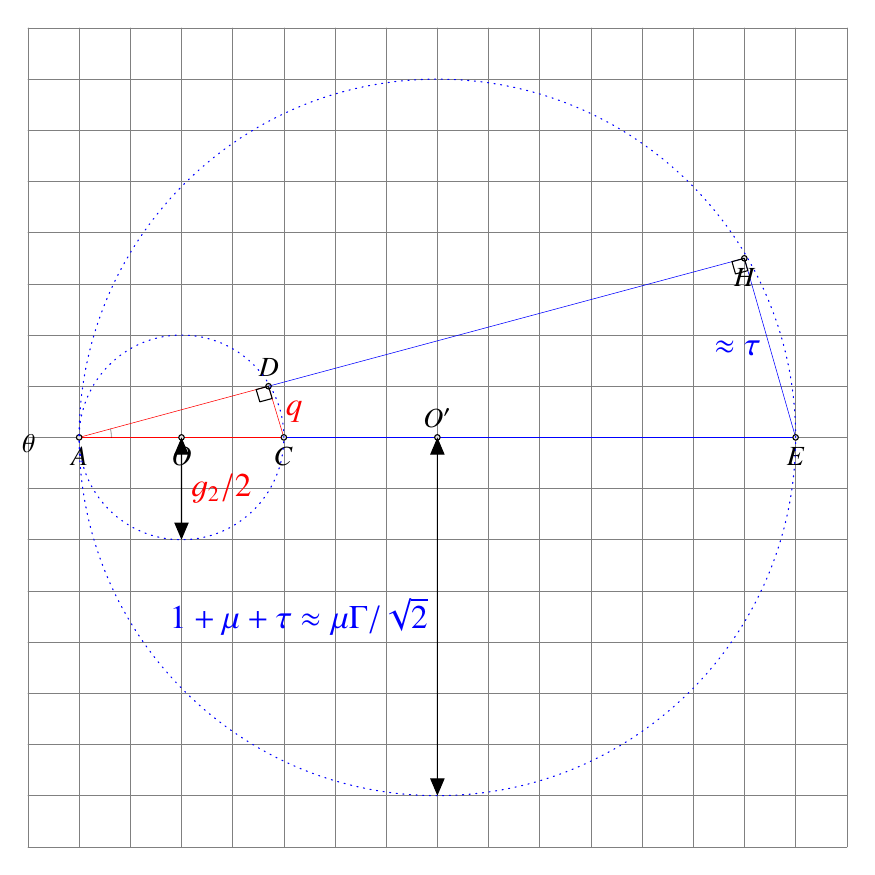
\begin{tikzpicture}[scale=0.65,line cap=round,line join=round,>=triangle 
45,x=1.0cm,y=1.0cm]
\draw[step=1cm,gray,very thin] (-5,-8) grid (11,8);
\tkzDefPoint(-4.,0.){A} 
\tkzDefPoint(0.,0.){C}
\tkzDefPoint(3.,0.){O'}
\tkzDefPoint(10.,0.){E}
\tkzDefMidPoint(A,C) \tkzGetPoint{O}
\tkzInterLC[R](A,C)(C,-0.3cm) \tkzGetSecondPoint{B}
\tkzInterLC[R](C,E)(E,-1cm) \tkzGetSecondPoint{F}
%\tkzDefLine[orthogonal=through D](A,D)
\tkzDefLine[perpendicular=through F](O',E) \tkzGetPoint{G}
\tkzDefLine[perpendicular=through B](O,C) \tkzGetPoint{J}
\tkzDefMidPoint(F,G) \tkzGetPoint{H}
\tkzDefMidPoint(J,B) \tkzGetPoint{D}
%\tkzInterLC(D,tkzPointResult)(O,A) \tkzGetSecondPoint{C}
%\tkzInterLC(F,tkzPointResult)(B,E) \tkzGetSecondPoint{G}
%\tkzDrawPolygon(A,E,H)
\tkzDrawSegment[color=blue](H,E)
\tkzDrawSegment[color=blue](H,D)
\tkzDrawSegment[color=blue](C,E)
\tkzDrawSegment[color=red](A,C)
\tkzDrawSegment[color=red](D,A)
\tkzDrawSegment[color=red](C,D)
\tkzDrawPoints(A,C,D,O,O',E,H)
\tkzLabelPoints(A,C,O,E,H)
\tkzLabelPoints[above](O',D)
%\tkzLabelPoints[left](D)
\coordinate (center) at (O);
\coordinate (center1) at (O');
\draw[blue, dotted]
      let \p1 =  ($(C)-(center)$),
          \n0 = {veclen(\x1,\y1)}
      in (center) circle(\n0);
\draw[blue, dotted]
      let \p1 =  ($(E)-(center1)$),
          \n0 = {veclen(\x1,\y1)}
      in (center1) circle(\n0);
%\draw [<->] (-1.8,1.7) node[right]{} -- (O) node[left]{};
\node [anchor = east,text=blue] at (3.,-3.5) {\large $1+\mu+\tau \approx \mu \Gamma /\sqrt2$};
\draw [<->] (O') node[left]{} -- (3.,-7.) node[right]{};
\node [anchor = west,text=red] at (-2.,-1.) {\large $g_2/2$};
\draw [<->] (O) node[left]{} -- (-2.,-2.) node[right]{};
\tkzMarkRightAngle(A,H,E)
\tkzMarkRightAngle(A,D,C)
\tkzDefMidPoint(H,E) \tkzGetPoint{I}
\tkzLabelSegment[left,text=blue](H,E){\large $\approx \tau $}
\tkzLabelSegment[right,text=red](D,C){\large $q$}
%\tkzMarkAngle[fill=blue!20,size=0.4cm,opacity=.5](E,A,H)
%\tkzLabelAngle[pos=1.4](E,A,H){$\theta$}
    \begin{pgfinterruptboundingbox}
        \tkzMarkAngle[fill = gray, size=0.633cm, opacity = .3](C,A,D)
        \tkzLabelAngle[pos = 1.](D,A,C){$\theta$}
    \end{pgfinterruptboundingbox}
\end{tikzpicture}
\caption[Weinberg-Koide Circles]{Weinberg-Koide similitude circles. Figure not drawn to scale.}
\label{WeinbergKoideCircles}
\end{figure}



\subsection{La relation de Koide des trois fermions principaux}
L'Axe Topologique est dévolu aux bosons, mais les deux fermions exotiques principaux, le muon et le tau, apparaisent par leur rapport, pour k = 1, c'est-à-dire dans les 6 dimensions cachées des cordes: $\tau/\mu \approx g(1) \approx 2 a_s$. où $\mu$ et $\tau$ sont les rapports de masse des fermions muon et tau par rapport à l'électron, qui sont les correspondants de l'électron dans les deux "générations apparemment inutiles" des particules. L'étude des déviations conduit à la relation (1 ppm):

\begin{equation}
2 a_s \approx \beta^4 \sqrt{f(1)\tau/\mu}  
\end{equation}

La valeur précise de $\tau$ est déduite de la formule empirique suivante de Koide, et de la relation $l_{nl}/P\lambdabar_e \approx \mu^2/a \approx \sqrt{(a_w/pH)}$ précisant, au ppb près, la mesure, déjà à 10 ppb, du rapport de masse muon-électron. On observe qu'elle fait intervenir la constante d'Atiyah, à 6 ppm près: 


\begin{equation}
(1+\mu+\tau) = (2/3)(1+\sqrt\mu+\sqrt\tau)^2 \approx \Gamma (H/p)^2 / \sqrt 2 
\end{equation}

Cette relation, liée aux propriétés des "matrices circulantes", ne reçoit aucune explication dans le modèle standard, qui manifeste, là encore, son insuffisance.
Cette formule de Koide s'est révélée prédictive à une époque où la mesure de $\tau$ était fausse de $3 \sigma$. La valeur optimale de $\tau$ a été déduite \cite{Sanchez2} de cette formule. 

Le rapport $\tau/(2\times (1+\mu+\tau) = \sin\theta_{\tau} $ est très voisin de $\sin\theta$ (Table \ref{tab:2:table2}). Il corrèle directement avec les couplages $a_w$ et $P$ (12 ppb):

\begin{equation}
a_{w} \sin \theta_{\tau} \approx \sqrt{P} (H/p_W)^4
\end{equation}

où $p_W = 6\pi^5$ est le rapport de Wyler, avec une valeur de $\pi$ très proche (2 ppb) de la valeur théorique.

%On observe que $1-\cos\theta_{\tau} \approx 1/a_s$, tandis que le terme symétrique $1+\cos\theta_{\tau}$ correspond au développement singulier suivant:

%\begin{equation}
 %1+\cos\theta_{\tau} \approx \tau/(4\pi_{\tau})^2\sqrt a ~~~~ \rightarrow ~~ \pi_{\tau} : 3, 7, \sqrt a
%\end{equation}

%\textit { $\sqrt a$ étant le terme générateur de l'électrodynamique quantique des diagrammes de Feynman, la pertinence de la rationalisation symbolique de $\pi$ ne %peut être niée.}







 

 Le cercle circonscrit du triangle de Weinberg (Figure 4) fait apparaître le nombre musical $2^{1/12}$, qui est voisin de: 
 
 \begin{equation}
2^{1/12} \approx (1+\mu+\tau)/\tau
 \end{equation}
 
 Cette corrélation répertoriée \cite{Sternheimer} explique la conjonction ci-dessus des deux cercles Weinberg-Koide.
 %L'ordinateur indique la double ppb-connexion avec le rapport de "normalisation" d'Atiyah, faisant apparaître la base optimale $e$:
 
  %\begin{equation}
%a/\Gamma = \pi/\gamma \approx e2d_e (6\pi_{16}^5/p)^2 \approx  2 sin~\theta ~(WZ/p_0p\tau)^2
 %\end{equation}
 
 %où $ 2d_e $ est le moment magnétique relatif de l'électron, $ \pi_{16}= 3+1/(7+1/16) = 335/113$ et $p_0 = 2\times 30 \times 31 = 1831$. Cette formule confirme \textit{la prédiction d'Eddington, la symétrie proton-tau, complètement ignorée par le modèle standard, oubliant le fait qu'Eddington avait prédit le tau 35 ans avant sa découverte, avec une bonne estimation de sa masse \cite{Eddington}.}
 
 
 %L'écart suivant est significatif:
 
%\begin{equation}
%\sin \theta^2 - \sin \theta_{\tau}^2  \approx 1/\sqrt a_w \sin_{eff}{\theta} (m_Z) \approx 1 / P^{1/4}
 %\end{equation}
  
 %faisant apparaître le terme $\sin_{eff}{\theta} (m_Z)$ appelé "effective weak mixing angle"  (Table \ref{tab:2:table2}).
 
% Dans un monde arithmétique, on s'attend à ce que $\delta = a - 137 $ intervienne, en effet, à 0.4 ppm près:

%\begin{equation}
%((1+\mu+\tau)/\mu)^2 = (\Gamma/\sqrt 2)(q'/\delta)(H^3/p^2n_t) 
%\end{equation}

%confirmant ainsi la relation ci-dessus, en la reliant à $q'$, ce qui valide ainsi les valeurs de $W$ et $Z$ à mieux que le ppm.


 




 
 
 
 

\begin{figure}
\centering
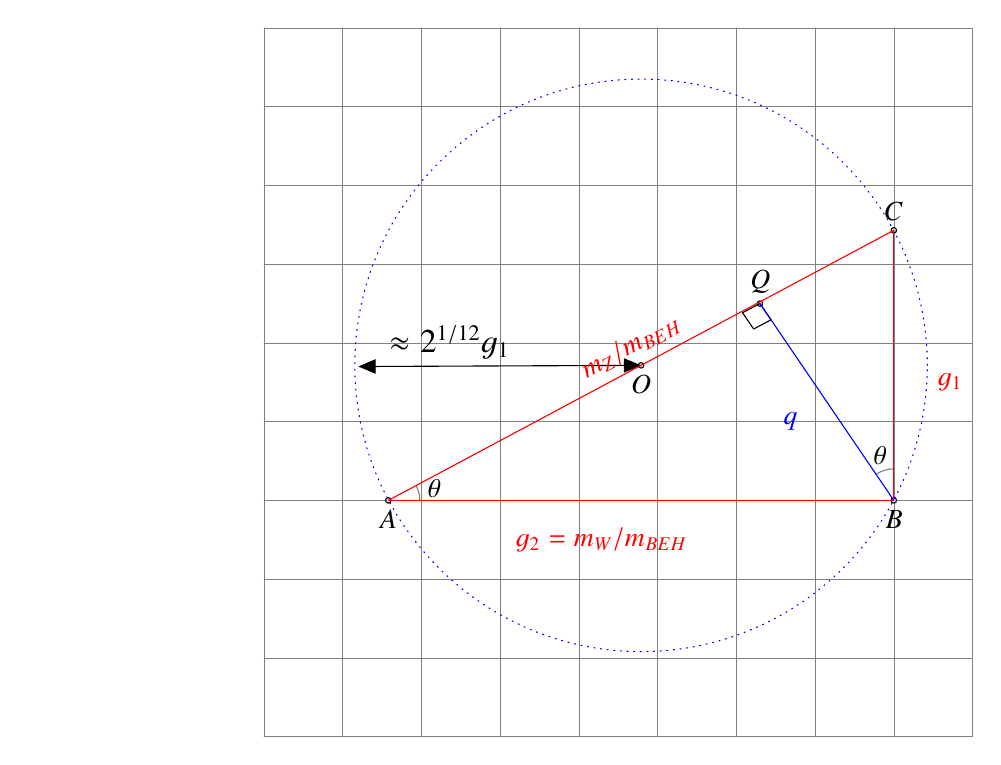
\begin{tikzpicture}[scale=1.0,line cap=round,line join=round,>=triangle 
45,x=1.0cm,y=1.0cm]
%\label{tab:14:table14}
\draw[step=1cm,gray,very thin] (-3,-3) grid (6,6);
\tkzDefPoint(-1.42,0.0){A} \tkzDefPoint(5.,3.43){C} \tkzDefPoint(5.,0.){B} \tkzDefPoint(3.3,2.5){Q}
\tkzDrawPoints(A,C,B,Q)
\tkzMarkRightAngle(A,Q,B)
\tkzLabelPoints[below](A,B)
\tkzLabelPoints[above](C,Q)
\tkzMarkAngle[fill=blue!20,size=0.4cm,opacity=.5](B,A,C)
\tkzLabelAngle[pos=0.6](B,A,C){$\theta$}
\tkzDefMidPoint(A,C) \tkzGetPoint{O}
\coordinate (center) at (O);
\tkzLabelPoints[below](O)
\tkzDrawPoints(O)
\draw [<->] (-1.8,1.7) node[right]{} -- (O) node[left]{};
\tkzLabelSegment[sloped,right,above,text=red](A,C){$m_Z/m_{BEH}$}
\draw[blue, dotted]
      let \p1 =  ($(C)-(center)$),
          \n0 = {veclen(\x1,\y1)}
      in (center) circle(\n0);
\tkzMarkAngle[fill=blue!20,size=0.4cm,opacity=.5](C,B,Q)
%\tkzMarkAngle[fill=blue!20,size=0.4cm,opacity=.5](O,E,D')
\tkzLabelAngle[pos=0.6](C,B,Q){$\theta$}
\draw[color=red] (-1.42,0.) -- (5.,0.);
\draw[color=red] (5.,0.) -- (5.,3.43);
\draw[color=red] (-1.42,0.) -- (5.,3.43);
\draw[color=blue] (5.,0.) -- (3.3,2.5);
\node [anchor = east,text=blue] at (3.9,1.0) {$q$};
\node [anchor = east,text=red] at (6.,1.5) {$g_1$};
\node [anchor = east,text=red] at (2.5,-0.5) {$g_2 =m_W/m_{BEH}$};
\clip(-6.,-0.4) rectangle (0.4,3.4);
\draw[color=black] (-0.5,2.0) node {\large $\approx 2^{1/12} g_1 ~~$};
\end{tikzpicture}
\caption[Weinberg Triangle]{Weinberg Triangle.}
\label{WeinbergTriangle}
\end{figure}









\begin{figure}
\centering

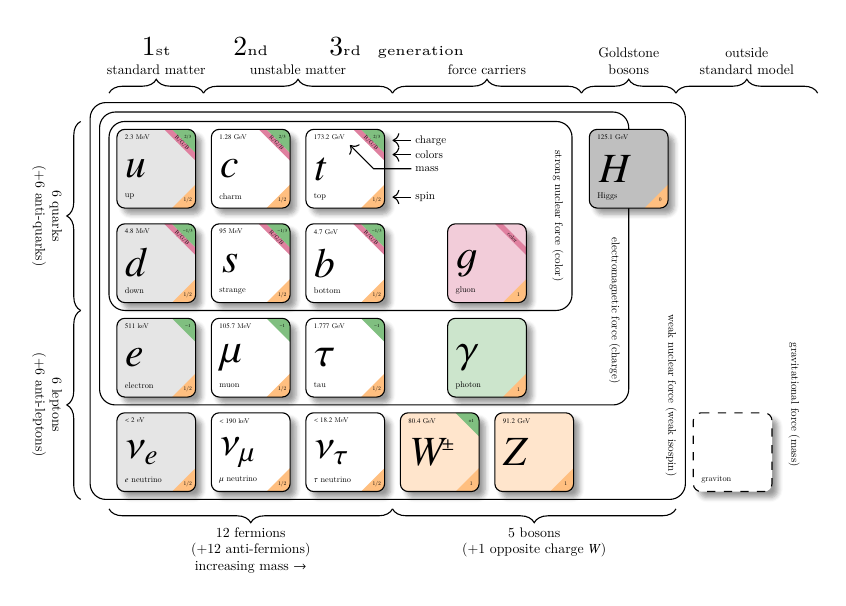
\begin{tikzpicture}[x=1.2cm, y=1.2cm]
  \draw[round] (-0.5,0.5) rectangle (4.4,-1.5);
  \draw[round] (-0.6,0.6) rectangle (5.0,-2.5);
  \draw[round] (-0.7,0.7) rectangle (5.6,-3.5);

  \node at(0, 0)   {\particle[gray!20!white]
                   {$u$}        {up}       {$2.3$ MeV}{1/2}{$2/3$}{R/G/B}};
  \node at(0,-1)   {\particle[gray!20!white]
                   {$d$}        {down}    {$4.8$ MeV}{1/2}{$-1/3$}{R/G/B}};
  \node at(0,-2)   {\particle[gray!20!white]
                   {$e$}        {electron}       {$511$ keV}{1/2}{$-1$}{}};
  \node at(0,-3)   {\particle[gray!20!white]
                   {$\nu_e$}    {$e$ neutrino}         {$<2$ eV}{1/2}{}{}};
  \node at(1, 0)   {\particle
                   {$c$}        {charm}   {$1.28$ GeV}{1/2}{$2/3$}{R/G/B}};
  \node at(1,-1)   {\particle 
                   {$s$}        {strange}  {$95$ MeV}{1/2}{$-1/3$}{R/G/B}};
  \node at(1,-2)   {\particle
                   {$\mu$}      {muon}         {$105.7$ MeV}{1/2}{$-1$}{}};
  \node at(1,-3)   {\particle
                   {$\nu_\mu$}  {$\mu$ neutrino}    {$<190$ keV}{1/2}{}{}};
  \node at(2, 0)   {\particle
                   {$t$}        {top}    {$173.2$ GeV}{1/2}{$2/3$}{R/G/B}};
  \node at(2,-1)   {\particle
                   {$b$}        {bottom}  {$4.7$ GeV}{1/2}{$-1/3$}{R/G/B}};
  \node at(2,-2)   {\particle
                   {$\tau$}     {tau}          {$1.777$ GeV}{1/2}{$-1$}{}};
  \node at(2,-3)   {\particle
                   {$\nu_\tau$} {$\tau$ neutrino}  {$<18.2$ MeV}{1/2}{}{}};
  \node at(3,-3)   {\particle[orange!20!white]
                   {$W^{\hspace{-.3ex}\scalebox{.5}{$\pm$}}$}
                                {}              {$80.4$ GeV}{1}{$\pm1$}{}};
  \node at(4,-3)   {\particle[orange!20!white]
                   {$Z$}        {}                    {$91.2$ GeV}{1}{}{}};
  \node at(3.5,-2) {\particle[green!50!black!20]
                   {$\gamma$}   {photon}                        {}{1}{}{}};
  \node at(3.5,-1) {\particle[purple!20!white]
                   {$g$}        {gluon}                    {}{1}{}{color}};
  \node at(5,0)    {\particle[gray!50!white]
                   {$H$}        {Higgs}              {$125.1$ GeV}{0}{}{}};
  \node at(6.1,-3) {\particle
                   {}           {graviton}                       {}{}{}{}};

  \node at(4.25,-0.5) [force]      {strong nuclear force (color)};
  \node at(4.85,-1.5) [force]    {electromagnetic force (charge)};
  \node at(5.45,-2.4) [force] {weak nuclear force (weak isospin)};
  \node at(6.75,-2.5) [force]        {gravitational force (mass)};

  \draw [<-] (2.5,0.3)   -- (2.7,0.3)          node [legend] {charge};
  \draw [<-] (2.5,0.15)  -- (2.7,0.15)         node [legend] {colors};
  \draw [<-] (2.05,0.25) -- (2.3,0) -- (2.7,0) node [legend]   {mass};
  \draw [<-] (2.5,-0.3)  -- (2.7,-0.3)         node [legend]   {spin};

  \draw [mbrace] (-0.8,0.5)  -- (-0.8,-1.5)
                 node[leftlabel] {6 quarks\\(+6 anti-quarks)};
  \draw [mbrace] (-0.8,-1.5) -- (-0.8,-3.5)
                 node[leftlabel] {6 leptons\\(+6 anti-leptons)};
  \draw [mbrace] (-0.5,-3.6) -- (2.5,-3.6)
                 node[bottomlabel]
                 {12 fermions\\(+12 anti-fermions)\\increasing mass $\to$};
  \draw [mbrace] (2.5,-3.6) -- (5.5,-3.6)
                 node[bottomlabel] {5 bosons\\(+1 opposite charge $W$)};

  \draw [brace] (-0.5,.8) -- (0.5,.8) node[toplabel]         {standard matter};
  \draw [brace] (0.5,.8)  -- (2.5,.8) node[toplabel]         {unstable matter};
  \draw [brace] (2.5,.8)  -- (4.5,.8) node[toplabel]          {force carriers};
  \draw [brace] (4.5,.8)  -- (5.5,.8) node[toplabel]       {Goldstone\\bosons};
  \draw [brace] (5.5,.8)  -- (7,.8)   node[toplabel] {outside\\standard model};

  \node at (0,1.2)   [generation] {1\tiny st};
  \node at (1,1.2)   [generation] {2\tiny nd};
  \node at (2,1.2)   [generation] {3\tiny rd};
  \node at (2.8,1.2) [generation] {\tiny generation};
\end{tikzpicture}
\caption[Standard Model of Particle Physics.]{Standard Model \cite{Burgard} \footnote{A standard diagram of the current standard model of physics. In some ways, this was the ultimate, single-diagram user experience challenge: all of our current understanding of the universe condensed into a single infographic. This improved diagram of the standard model of physics was made at the CERN Webfest 2012 by David Galbraith and Carsten Burgard. Source: http://davidgalbraith.org/portfolio/ux-standard-model-of-the-standard-model/ . Programmed in TikZ by Carsten Burgard. TikZ styles syntax by Stefan Kottwitz.}} 
\label{StandardModel}
\end{figure}








 
 
 \begin{figure}
\centering
\begin{tikzpicture}[scale=0.75]
%\tkzInit[xmax=6.4, zmax=3.4]
\tkzDefPoint(0.0,0.0){A} \tkzDefPoint(6.4,0.0){B} \tkzDefPoint(5.1,-1.3){C} \tkzDefPoint(4.0,-1.0){q}
\tkzDrawPoints(A,B,C,q)
\tkzDefMidPoint(B,q) \tkzGetPoint{D}
%\tkzDefPoint[label={[align=left]right:$q$},xshift=00mm](4.5,-0.5){D}
\tkzLabelSegment[sloped,text=red,xshift=-06mm](q,B){$q$}
\tkzMarkRightAngle(A,B,C)
\tkzMarkRightAngle(B,q,C)
\tkzLabelPoints[below](A,B,C)
%\tkzLabelPoints[above right](q)
\tkzMarkAngle[fill=blue!40,size=1.4cm,opacity=.5](C,A,B)
\tkzLabelAngle[pos=1.6](C,A,B){$\theta$}
    %\draw [important line] (0.0,0.) coordinate (A) -- (5.1,-1.3) coordinate (C) node[below, text width=5em] {}
    %\draw [blue] (6.4,0.) coordinate (A) -- (4.,-1.0) coordinate (D) node[below, text width=5em] {$h$}
    %\draw [red] (6.4,0.) coordinate (B) -- (4.,-1.0) coordinate (D) node[below, text width=5em] {$q$}
  \draw (6.4,0,0) coordinate (x) |- (0,10,0) coordinate [midway] (h) coordinate (y) -- (0,10,3.4) coordinate (a) -- (0,0,3.4) coordinate (z) -- (6.4,0,3.4) edge (x) -- (6.4,10,3.4) coordinate (v) edge (h)
  -- (a)  ;
  \draw [dashed] (0,0,0) coordinate (o) edge (x) edge (y) -- (z);
  \draw [dashed] (0,0,0) coordinate (o) edge (x) edge (v) -- (v);
  \draw [blue] (0,0,0)  -- (6.4,0.0,3.4);
  \draw [red] (4.9,0.02,2.7)  -- (6.4,0.0,0.0);
  %\node [circle, minimum size=2pt, inner sep=0pt, fill, label=135:$\sqrt{2a^3/pp_G}$] at (v) {};
  \draw [very thin,black,line join=round] (0,0,0)  -- node [sloped,above] {$\sqrt{2a^3/pp_G}$} (6.4,10,3.4);
  \node [circle, minimum size=4pt, inner sep=0pt, fill, label=135:o] at (o) {};
  \draw [decoration={markings,mark=at position 1 with
    {\arrow[scale=3,>=stealth]{>}}},postaction={decorate}] (0,0,0) -- (6.4,10,3.4);
  \draw [dashed] (0,0,0) -- (6.4,0,3.4);
  \draw [->] (x) -- +(3pt,0,0) node [midway,above] {$g_2$};
  \draw [->] (y) -- +(0,3pt,0) node [midway,right] {$1$};
  \draw [->] (z) -- +(0,0,3pt) node [midway,above] {$g_1$};
  %\draw (v) -- ++(0,0,-2) coordinate (d) -- ++(-2,0,0) coordinate (e) -- ++(0,0,2) |- ++(2,-2,0) coordinate [midway] (f) -- ++(0,0,-2) coordinate (g) -- (d);
  %\draw [dashed] (e) -- ++(0,-2,0) coordinate (c) edge (f) -- (g);
  %\node [label=45:C] at (c) {};
  %\draw[red]   (0,0,0) -- (.95,0,0)    node[red,left=6pt]    {$x$};
\end{tikzpicture}
\caption[The Weinberg-Sanchez Cuboid]{3D "Weinberg-Sanchez" cuboid: 0.1 ppm Electro-weak / Gravitation connection}
\label{WeinbergSanchezCuboid}
\end{figure}






\begin{figure}
\centering
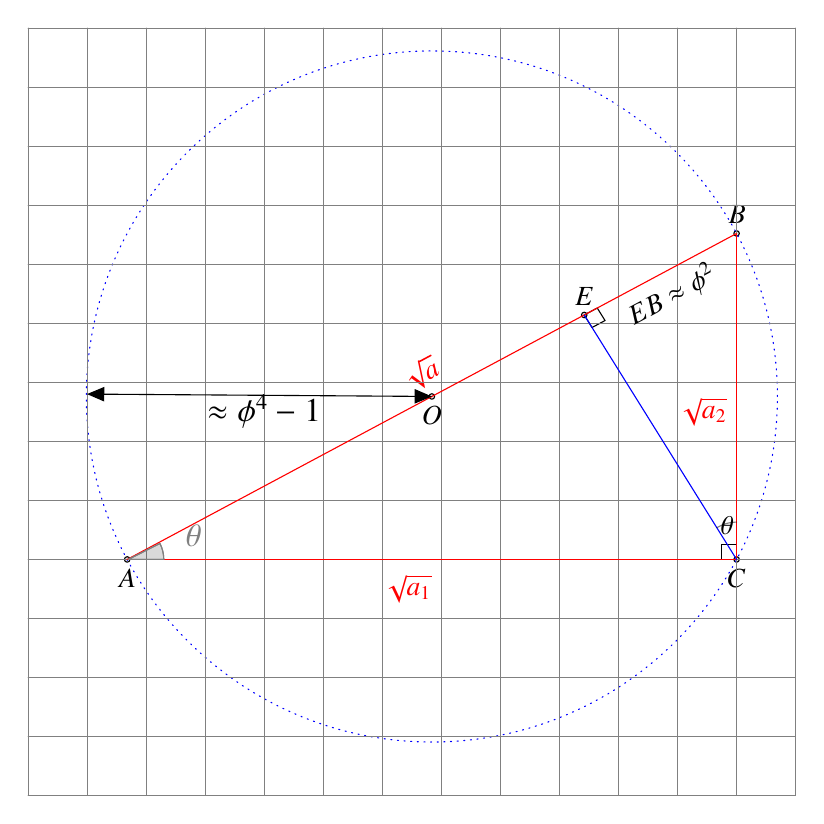
\begin{tikzpicture}[scale=0.75,line cap=round,line join=round,>=triangle 
45,x=1.0cm,y=1.0cm]
%\label{tab:13:table13}
\tkzDefPoint(-4.32,0.0){A} \tkzDefPoint(6.0,5.52){B} \tkzDefPoint(6.,0.){C} %\tkzDefPoint(0.0,0.0){D}
\tkzDrawPoints(A,B,C)
\tkzMarkRightAngle(B,C,A)
%\tkzMarkRightAngle(B,D,C)

\tkzLabelPoints[below](A,C)
\tkzLabelPoints[above](B)
\tkzDefMidPoint(A,B) \tkzGetPoint{O}
\coordinate (center) at (O);
\tkzLabelPoints[below](O)
\tkzDrawPoints(O)
%\tkzDefInterPoint(A,C) \tkzGetPoint{O}
\tkzLabelSegment[sloped,above,text=red](A,B){$\sqrt{a}$}
\draw[blue, dotted]
      let \p1 =  ($(-4.32,0)-(center)$),
          \n0 = {veclen(\x1,\y1)}
      in (center) circle(\n0);
\tkzDefMidPoint(O,B) \tkzGetPoint{E}
\tkzDrawPoints(E)
\tkzLabelPoints[above](E)
\tkzMarkRightAngle(B,E,C)
\draw[step=1cm,gray,very thin] (-6,-4) grid (7,9);
\draw[color=red] (-4.32,0.) -- (6.,0.);
\draw[color=red] (6.,0.) -- (6.,5.52);
\draw[color=red] (-4.32,0.) -- (6.,5.52);
\draw[color=blue] (E) -- (C);
\tkzDefMidPoint(E,B) \tkzGetPoint{F}
\tkzLabelSegment[sloped,below,text=black](E,B){$EB \approx \phi^{2}$}
\tkzMarkAngle[fill=blue!20,size=0.633cm,opacity=.5](B,C,E)
\tkzLabelAngle[pos=0.6](B,C,E){$\theta$}
%\node [anchor = east] at (1.,3.5) {$\sqrt{a}$};
\node [anchor = east,text=red] at (6.,2.5) {$\sqrt{a_2}$};
\node [anchor = east,text=red] at (1.,-0.5) {$\sqrt{a_1}$};
\draw [<->] (O) node[left]{} -- (-5.0,2.8) node[right]{};
\clip(-6.,-0.4) rectangle (0.4,3.4);
\draw [shift={(-4.3,0.)},color=gray,fill=darkgray,fill opacity=0.1] (0,0) -- (0.:0.6) arc (0.:26.9:0.6) -- cycle;
\draw [shift={(-4.3,0.)},color=gray,fill=darkgray,fill opacity=0.1] (0,0) -- (0.:0.6) arc (0.:26.9:0.6) -- cycle;
%\draw[color=gray,fill=darkgray,fill opacity=0.1] (0.,0.42) -- (-0.42,0.42) -- (-0.42,0.) -- (0.,0.) -- cycle; 
%\draw (0.,6.)-- (-4.32,0.);
%\draw (6.,5.52)-- (-4.32,0.);
%\draw (6.,0.)-- (6.,5.52);
\draw[color=gray] (-3.2,0.4) node {\large $\theta$};
\draw[color=black] (-2.,2.5) node {\large $\approx \phi^4-1$};
\draw[color=gray] (0.34,0.33);
%\tkzMarkRightAngle[fill=blue!20](B,F,C)
\end{tikzpicture}
\caption[Electric Triangle properties]{Electric Triangle.}
\label{ElectricTriangle}
\end{figure}




  





%La charge électrique $q = \sqrt{4\pi/a} $ montre une connection avec la forme trigonométrique \cite{Sanchez2} $a \approx 44\pi - \arccos(1/e)$

%\begin{equation}
%a \approx 44\pi_a + \ln(\sqrt {4\pi_a/a})     ~~~~ \rightarrow 6\pi_a^5 \approx p ~~~~ \rightarrow \pi_a : 3, 7, e^e + 1
 %\end{equation}

%Ainsi la charge électrique $q$  est intimement reliée au couplage électrique $\sqrt a$. Le triangle représentatif de ce dernier montre une %nette connexion avec les puissances 2 et 4 du nombre d'or \cite{Sanchez1}.






%\begin{equation}
%q \times 495 \approx 150 = u_0^2d_0 \approx p^{2/3}
%\end{equation}

%\begin{equation}
%f(8)/q  \approx 180 = u_0d_0^2 \approx (n_t/a)^2
%\end{equation}

%Les masses équivalentes des quarks apparaissent dans la double connexion avec le boson scalaire $H^{(0)}$ et le Nombre Holique $210^{210}$, %(168 et 20 ppm):

%\begin{equation}
%210^{210} p_G /a^{3/2}  \approx (p_G -\tau/H)^{u^2d-1/2} \approx (H^0)^{(ud^2+1)/2}
%\end{equation}



%Avec le terme topologique fondamental $f(2) = e^{\sqrt2}$, la masse de la corde, on observe, à 7 et 30 pm près:

%\begin{equation}
%a^2 f(1)/137 q  \approx 9\mu \approx \tau ~tg~\theta
%\end{equation}

%\textit{La charge électrique relie donc la fonction topologique à la physique des particules.}
 


%\subsection{Connexions avec le générateur de Lucas-Lehmer et les "nombres économiques"}

%Le générateur de Lucas-Lehmer est le nombre $(2 + \sqrt 3)$, lié à $a$ et $a^a$, ce dernier terme étant aussi lié au générateur de Pell-Fermat $(1 + \sqrt2)$ \cite{Sanchez2}. Les puissances de type $2^n$ de ce générateur produisent des nombres dont la partie entière est la série de Lucas-Lehmer, qui permet de déterminer si un nombre de type Mersenne $2^n-1$ est premier. Ce générateur se caractérise par:


%\begin{equation}
%(2 + \sqrt 3) + 1/ (2 + \sqrt 3) = 4
%\end{equation}


%On observe, à 20 ppb:

%\begin{equation}
%(2\cot\theta) + 1/(2\cot\theta) \approx \sqrt{4^2 + (1/5)^2}
%\end{equation}

%ce qui semble impliquer l'espace 5D prévu par Eddington, en réinterprétant l'algèbre de Dirac.

%De plus, on observe la connexion suivante impliquant la fonction topologique $f(d) = exp(2^{d/4})$ et $136$, la première estimation
%d'Eddington pour $a$:

%\begin{equation}
%(q\cos\theta + 1/q\cos\theta )/4 \approx f(-a/4d_e)    \approx (2(a-136))^{1/(2\times 137)}
%\end{equation}

%tandis que:

%\begin{equation}
% 1/q\cos\theta \approx e^{2a /(\mu+1)}    \approx (2+\sqrt3)(2a^3p/H^2n)^{1/a}
%\end{equation}

%de sorte qu'on retrouve un terme analogue à la racine holique ci-dessus du rayon de Hubble. 

\textit{Le triplet $136-137-a$ est vraiment au centre de l'Arithmétique Cosmique}. En effet, d'après Salingaros \cite{Salingaros}: \textit{Indeed, it seems that Eddington was really ahead of his time : Eddington anticipated results of current interest. He discovered the Majorana spinors, and was responsible for the standard $\gamma^5$ notation as well as the notion of chirality. Furthermore, Eddington defined Clifford algebras in eight and nine dimensions which are now appearing in grand unified gauge and supersymmetric theories. A point which Eddington cleared up, yet is still misunderstood, is that the Dirac algebra corresponds to a five-dimensional base space.}


%Le caractère "monstrueux" de $a$ est qu'il apparait comme exposant dans la triple relation suivante (écarts -1.69, -1.73 et 0.01 $\times 10^{-3}$, impliquant le nombre "économique" géant  $ E = exp(exp(e^e))$, qui et relié à $a$, $P$ et $\sin \theta$:


%\begin{equation}
 %\left\{
   % \begin{array}{ll}
      %  E = exp(exp(e^e))\approx (\tau^{\tau})^{e^6/3} \approx e^{a(2e^e)^3}   \\
      %  P^4  \approx E^{1/(a-1)^2} \approx (9/2)^a \approx (1/\sin \theta)^{2d_ea}/d_e^4 
   % \end{array}
%\right.
%\end{equation}


%où $2d_e$ est le moment magnétique de l'électron. Ainsi le lepton terminal $\tau \approx e^{3e}$ apparait-il comme un élément simplificateur dans des relations "économiques" alors que, comme vu plus haut, le lepton intermédiaire $\mu$ a une signification directement holique. Cela appelle des approfondissements dans ces deux voies de recherche. 








 
 
 
 
 
 
\section{Prédictions et Conclusions: vers l'Unification Arithmétique}
Le modèle standard des particules, en particulier à travers ses charges de jauge $q'$ et $q''$, confirme la fonction topologique et la Cosmologie Permanente. Mais celles-ci vont au-delà, en affectant \textit{une masse à la corde, ainsi qu'aux gluons, photon et graviton}. Nous prévoyons que la mission Euclide, consacrée à la supposée variation, par tranche d'un milliards d'années-lumière, du taux de matière sombre, devrait constater \textit{une invariance du taux de matière sombre au lieu de la décroissance attendue}. Le futur télescope infra-rouge Webbs, consacré à la formation des galaxies lointaines, devrait constater \textit{une profusion inattendue de vieilles galaxies à longue distance.}

Indépendamment de la Cosmologie, les matrices circulantes de Koiré montrent aussi des limites du modèle standard actuel.

Le physicien E.Schrödinger \cite{Schroedinger} avait anticipé l'existence d'une mémoire moléculaire, qui s'est révélée dans la double hélice de l'ADN. De la présente étude, il ressort le rôle central de la masse du bi-codon d'ADN, voisine de $m_H^2/m_e$, qui est définie à 3 atomes d'Hydrogène près \cite{Sanchez3}. En effet, elle occupe la place centrale $d = 16$ dans l'Axe Topologique, et figure dans la progression double de Fibonacci: 2(corde), $4(2\sqrt{\Phi_s a_s)}$, 6 (gluon), 10(atome), 16(ADN), 26(Univers). 
Contrairement à la thèse du Multivers, basée sur une indépendance entre lois physiques et biologique et sur une mauvaise interprétation du principe anthropique, la biologie s'intègre dans le Cosmos calculateur, la molécule d'ADN devant être un calculateur-hologramme-ligne.


\textit{Le rôle central de la masse du bi-codon d'ADN, à la fois dans les équation holiques et dans l'Axe Topologique annonce enfin l'unification physique-biologie.} 
\textit{Plus qu'une simple mémoire, l'ADN serait un centre de calcul, utilisant, comme le Cosmos, la base arithmétique optimale 3}.

Il a déjà été observé que l'ADN est parcouru par un courant électrique \cite{Montagnier}, ce qui confirme qu'il fonctionne comme un hologramme-ligne, capable d'envoyer des informations électro-magnétique dans l'environnement aqueux de l'organisme.

La relation, pour $k = 4, d= 18$, entre la température cosmique et celle des mammifères $T_{mam}\approx jT_C$, où $j = 8 \pi^2/ln2$ est la constante d'échelle de Sternheimer \cite {Sternheimer} prend toute son importance. Elle est très précise (37.2 Celsius). De plus, la longueur d'onde correspondante est très voisine de la moyenne entre le rayon de Hubble et la longueur de Planck, tandis qu'avec le rayon holographique réduit $R_N$ du Cosmos on obtient le point triple de l'Eau, lequel est très voisin de $T_{H^2}T{O^2}/T_C$, où les points triples de l'Hydrogène et de l'Oxygène sont impliqués.

\textit{ Alors que la chimie actuelle est incapable de calculer ces points triples, la cosmologie permanente montre clairement qu'ils sont connectés avec la température cosmique et celle des mammifères}. 


La relation $ln(4\pi (R_N/\lambda_{Wn})^2) \approx a$, précise à $10^{-5}$ près, montre que la longueur d'onde de Wien du rayonnement cosmique est centrale en Holographie cosmique. Ces relations sont beaucoup plus précises que les vagues assertions concernant le soi-disant "réglage fin" (fine tuning").  
 
%Le nombre d'or, par ses approximations remarquables $\Phi_s$ et $\Phi_a$, dont le rapport est $n(1-p/H)$, à 35 ppb près, apparait dans l'axe topologique %($\Phi_s$) et intervient par sa puissance holique 210 ($\Phi_a$).


L'apparition ancestrale du nombre d'or en biologie doit être prise au sérieux. Mais son role \textit{calculatoire} a été sous-estimé. Il apparaît clairement dans le "triangle électrique".

Les bases entières fondamentales 2,3, et 5 de la sensation musicale, respectivement liés aux spins 1/2, 1 et 2, sont reliés au Principe Holique. Mais comme le Nombre holique $210^{210}$ joue un rôle central dans cette étude, et qu'il contient $7^{210}$ il faut s'attendre à une particule de spin 3. 

\textit{Contrairement à la tendance actuelle de formalisation à outrance, les mathématiques doivent maintenant s’appuyer sur la physique de précision pour s'unifier, tout en liant Physique et Biologie.} 





%\begin{appendix}



%\listoftables{}   % table list
%\listoffigures{}  % figure list
%\section{Tables}

%\end{appendix}







%\end{document}











\section{L'exigence de quasi-continuité : la rationalisation symbolique}

Le propre de la Science est que l’on peut progresser sans connaître la théorie ultime, par approximations successives.  La non-reconnaissance de cette évidence historique a fait rejeter plusieurs théories et formules empiriques que le principe de rationalisation symbolique, en partculier de $\pi$, réhabilite pleinement. 

Une "exigence de quasi-continuité" a été présentée dans la conférence ANPA 1994 \cite{Sanchez1}, introduisant le Principe Holographique de manière beaucoup plus simple que celle d'autres théoriciens \cite{Hooft}. En effet, par opposition aux équations différentielles, qui sont fondamentalement inadaptées dans un monde quantique, comme Poincaré l'avait expressément souligné \cite{Poincare1}, \textit{les équations globales les plus simples} sont les connexions entre variétés topologiques de dimensions différentes (périmètre, aire, volume…), donc utilisent la constante $\pi$, et pourraient être liées aux symétries cristallines de dimensions supérieures, comme constaté ci-dessous.  

Dans cette hypothèse d’un Cosmos calculateur, de même qu’un ordinateur ne peut utiliser le $\pi$ mathématique "rigoureux", \textit {tout calcul doit être associé à une imprécision}. Dans cet article, la précision maximale $10^{-9}$ (ou ppb) est recherchée, laissant peu de prise au hasard. Ainsi $\pi$ \textit {doit} être rationalisé, et ce, dans un premier temps, de manière symbolique, c’est-à-dire que son développement fractionnaire doit montrer des paramètres-clefs (table 1).

\subsection{Le développement fractionnaire du $\pi$ mathématique}
En effet, le développement fractionaire du $\pi$ mathématique commence par les nombres 3, 7, 15, 1, 292.634591, ce dernier terme $\pi_5$ étant le rapport de masse neutron/électron $n$ divisé par $2\pi$, à 3 ppm près. Le rapport de masse proton-electron $p$ est doublement impliqué:

\begin{equation}
 \pi_5 \approx n/2\pi \approx p/2(3+1/(2\pi+1)) \approx p/2(3+1/(2w))
 \end{equation}
 
où $W_+ =  W_-$ et $Z$ sont les masses des trois bosons de jauge électrofaibles, rapportées à la masse de l'électron, $w = \sqrt a_w/W$ est un paramètre central dans la théories électrofaible rappelée ci-dessous, associé au paramètre $z = \sqrt a_w/Z$. On en déduit les relations ($7 \times 10^{-5}$ et $2 \times 10^{-3}$):
 
 
 \begin{equation}
 \left\{
    \begin{array}{ll}
        w \approx \pi + 1/2 \\
        z \approx ~ e + 1/2
    \end{array}
\right.
\end{equation}
 
 
montrant que \textit{le Cosmos utilise à la fois, et de manière symétrique, $\pi$ et la base néperienne $e$}. Noter que les séries de Riemann d'ordre paires utilisent effectivement des puissances de $\pi$, lequel se comporte donc bien comme une base de calcul. L'une des 31 formules donnant R (table 3) implique effectivement des puissances de $\pi$.



\subsection{Réhabilitation de la théorie de Wyler}
La base de calcul $\pi$ est confirmée par la théorie de Wyler \cite{Wyler}, qui aboutit à une formule approchant $p$ à 18 ppm près, repérée initialement par Lenz, dans un article célèbre d'une seule ligne \cite{Lenz}:

\begin{equation}
p_W = 6\pi^5
\end{equation}
 
Noter que cette expression est le produit aire-volume d'un cube de coté $\pi$. La théorie de Wyler conduit aussi à une expression pour $a$ faisant intervenir $\pi^{11}$ où 11 est la dimension de la supergravité. L'ordinateur confirme son implication, à $10^{-7}$ près: :

\begin{equation}
(3\sqrt a/4)^8 /120 \approx \pi^{11} \approx (P/a^2pn\mu)^5/(n_t \tau)^6
\end{equation}
 
ce qui s'écrit de manière holique, avec $\pi^{11} = \pi^{5}\pi^{6}$:

\begin{equation}
(\pi n_t \tau)^6 \approx (\pi a^2pn\mu)^5 \approx \Phi_a^{2\times 3\times 5 \times 6}
\end{equation}

faisant apparaître une aproximation $\Phi_a$ du nombre d'or. 

%telle que

%\begin{equation}
%\Phi_a^2/2 \approx (6\pi_a^5)^2/a^3  ~~~~ \rightarrow \pi_a = \sqrt {(a^2 - 137^2)}
%\end{equation}

%où la relation $a^2 \approx 137^2 + \pi^2$ a été soulignée par Atiyah \cite{Atiyah}. Une autre propriété liée à la théorie de Wyler est basée sur l'approximation $\pi \approx 4/\sqrt \Phi$ :

%\begin{equation}
%(4/\sqrt \Phi_a)^5/6 \approx (4\pi)^2 \sqrt a
%\end{equation}

\textit{Ainsi la théorie de Wyler, trop vite abandonnée par suite de l'utilisation exagérée du $\pi$ mathématique, relie $a$ et $\Phi_a$.}


\subsection{Le rayon de Hubble et $\pi$}
Les relations holographiques impliquant le rayonnement de fond conduisent à:

\begin{equation}
R/\lambdabar_e \approx (2\pi^2a^3)^5
 \end{equation}

où $2\pi^2a^3$ est l’aire de la sphère 4D de rayon $a$. Mais cette relation montre une imprécision de 565 ppm, voisine de $H/p_W$, à 1.5 ppm près. Et ce dernier écart est réduit au ppb si on considère la valeur suivante de $\pi$:

\begin{equation}
\pi_R = 3 + 1/(7+1/(16+2/e^{2e}))
\end{equation}

Noter que $H \approx 8e^{2e}$ à 33 ppm près. On retrouve ainsi, à $10^{-9}$ près, la valeur $R \approx 13.8119768$ milliards d’années-lumière:

\begin{equation}
R/\lambdabar_e  \approx 6H (2\pi_R a^3)^5      
\end{equation}

ce qui rétablit une symmétrie électron-hydrogène, conformément au modèle de la molécule gravitationnelle d’hydrogène.





\subsection{Le terme Lucasien du proton et $\pi$}
De plus, le terme Lucasien du proton $p_G = P/\sqrt {N_L}\approx 1831.531182$, où $N_L$ est le grand nombre de Lucas, le nombre premier le plus célèbre des l'histoire des mathématiques et le terme terminal de la Hiérarchie Combinatoire \cite{Bastin}, écrite sous la forme ci-dessus de Lenz-Wyler, présente un terme $\pi$ ayant un développement singulier: 

\begin{equation}
p_G = 6\pi_G^5~~~~ \rightarrow  ~~~~ \pi_G : 3, 7, 7, 7\sqrt 7 
\end{equation}

Cette formule confirme à 5 ppb près  l'étude d'optimisation antérieure de $G$ \cite{Sanchez2}, et réhabilite ainsi la théorie de Wyler, trop vite écartée, qui, précisément, implique un espace de dimension 7, caractéristique de l'algèbre des octonions. \textit{Atiyah avait effectivement prédit que la gravitation devait être liée à cet algèbre}\cite {Atiyah}. 


\subsection{Le terme Lucasien du proton et $e$}
Ce terme Lucasien $p_G$ se trouve aussi dans le développement suivant de la base naturelle des logarithmes, basé sur l'approximation $e \approx 19/7$, qui connecte avec l'approximation d'Archimède: $\pi \approx 22/7$. $e : 2, 7/5, -2^7$. Or $2^7/3 \approx \sqrt p$. On observe que le développement suivant approche $e$ à 2 ppb près.

\begin{equation}
e_G : 2, 7/5,  -3\sqrt{p_G} 
\end{equation}


\subsection{Le rayonnement de fond et $\pi$}
La longueur d'onde de Wien du rayonnement de fond vérifie (longueur fixe en Cosmologie Permanente, contrairement à la cosmologie standard):

\begin{equation}
\lambda_{Wn}/l_P \approx \pi_0^{64}~~~~ \rightarrow  ~~~~ \pi_0 : 3, 7, 16, 1, (W_+ + W_-)/Z ~~~~ \rightarrow  ~~~~ (W_+ + W_-)/Z = 2W/Z \approx (4\pi/\sqrt a)^8
\end{equation}

ce qui confirme la température cosmique optimale \cite{Sanchez2} dans le domaine du ppb. 

\textit{ Cette invariance de la température cosmique est contraire à la doxa officielle, mais seules les observations conformes au paradigme cosmologique dominant sont réellement publiées.}


\subsection{Le lepton Tau et $\pi$}

 $\tau$ étant le rapport de masse du fermion culminant Tau avec l'Electron, on observe le développement singulier suivant:  

\begin{equation}
 1+W/Z \approx \tau/(4\pi_{\tau})^2\sqrt a ~~~~ \rightarrow ~~ \pi_{\tau} : 3, 7, \sqrt a
\end{equation}

\textit {où $\sqrt a$ est le terme générateur de l'électrodynamique quantique des diagrammes de Feynman}.








%De plus, l'écart ci-dessus $e-2$ apparaît dans, à 30 ppb près:

%\begin{equation}
 %1+W/Z \approx 2(e-2)(1836p-3\times 137)/a^3
%\end{equation}






















\begin{figure}
\centering
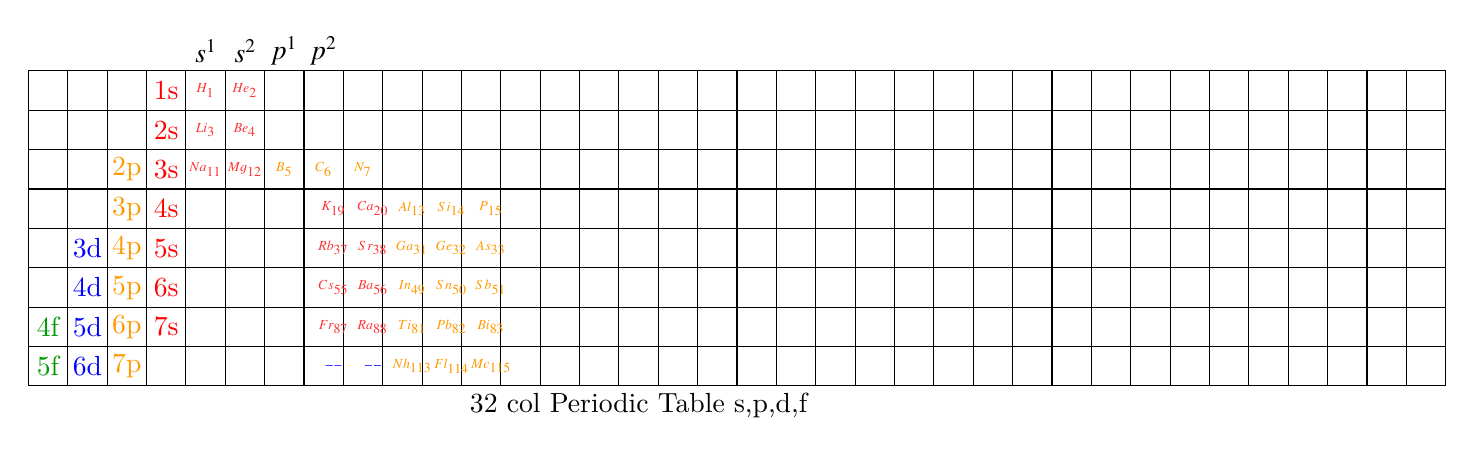
\begin{tikzpicture}[scale=.5]



  \begin{scope}[xshift=12cm]
    \draw (0, 0) grid (36, 8);
    %\draw[very thick, scale=3] (0, 0) grid (3, 3);

    \setcounter{row}{1}
    %\setrow { }{2}{ }  {5}{ }{1}  { }{9}{ }
    \setrow { } { }{ }{ }  {$s^1$}{$s^2$}{$p^1$}  {$p^2$}{}{}  { }{ }{ }  { }{ }{ }  { }{ }{ }
    \setrow { } { }{ }{\textcolor{red}{1s}}  { }{ }{ }  { }{ }{ }  { }{ }{ }  { }{ }{ }  { }{ }{ }

    \setrow { } { }{ }{\textcolor{red}{2s}}  { }{ }{ }  { }{ }{ }  { }{ }{ }  { }{ }{ }  { }{ }{ }
    \setrow { } { }{\textcolor{red!40!yellow}{2p}}{\textcolor{red}{3s}}  { }{ }{ }  { }{ }{ }  { }{ }{ }  { }{ }{ }  { }{ }{ }
    \setrow { } { }{\textcolor{red!40!yellow}{3p}}{\textcolor{red}{4s}}  { }{ }{ }  { }{ }{ }  { }{ }{ }  { }{ }{ }  { }{ }{ }

    \setrow { } {\textcolor{blue}{3d}}{\textcolor{red!40!yellow}{4p}}{\textcolor{red}{5s}}  { }{ }{ }  { }{ }{ }  { }{ }{ }  { }{ }{ }  { }{ }{ }
    \setrow { } {\textcolor{blue}{4d}}{\textcolor{red!40!yellow}{5p}}{\textcolor{red}{6s}}  { }{ }{ }  { }{ }{ }  { }{ }{ }  { }{ }{ }  { }{ }{ }
    \setrow {\textcolor{black!40!green}{4f}} {\textcolor{blue}{5d}}{\textcolor{red!40!yellow}{6p}}{\textcolor{red}{7s}}  { }{ }{ }  { }{ }{ }  { }{ }{ }  { }{ }{ }  { }{ }{ }
    \setrow {\textcolor{black!40!green}{5f}} {\textcolor{blue}{6d}}{\textcolor{red!40!yellow}{7p}}{ }  { }{ }{ }  { }{ }{ }  { }{ }{ }  { }{ }{ }  { }{ }{ }

    \node[anchor=center] at (15.5, -0.5) {32 col Periodic Table s,p,d,f};

    \begin{scope}[blue, font=\tiny]
      \setcounter{row}{1}
      %\setrow {H}{ }{6}  { }{7}{ }  {3}{ }{8}
      \setrow { } { }{ }{ }  { }{ }{ }  { }{ }{ }  { }{ }{ }
      \setrow { } { }{ }{ }  {\textcolor{white!20!red}{$H_1$}}{\textcolor{white!20!red}{$He_2$}}{ }  { }{ }{ }  { }{ }{ }  { }{ }{ }  { }{ }{ }

      \setrow { } { }{ }{ }  {\textcolor{white!20!red}{$Li_3$}}{\textcolor{white!20!red}{$Be_4$}}{ }  { }{ }{ }  { }{ }{ }  { }{ }{ }  { }{ }{ }
      \setrow { } { }{ }{ }  {\textcolor{white!20!red}{$Na_{11}$}}{\textcolor{white!20!red}{$Mg_{12}$}}{\textcolor{red!40!yellow}{$B_5$}}  {\textcolor{red!40!yellow}{$C_6$}}{\textcolor{red!40!yellow}{$N_7$}}{\textcolor{red!40!yellow}{$O_8$}}  {\textcolor{red!40!yellow}{$F_9$} }{\textcolor{red!40!yellow}{$Ne_{10}7$} }{ }  { }{ }{ }  { }{ }{ }
      \setrow { } { }{ }{ }  {\textcolor{white!20!red}{$K_{19}$}}{\textcolor{white!20!red}{$Ca_{20}$}}{\textcolor{red!40!yellow}{$Al_{13}$}}  {\textcolor{red!40!yellow}{$Si_{14}$}}{\textcolor{red!40!yellow}{$P_{15}$}}{ }  { }{ }{ }  { }{ }{ }  { }{ }{ }

      \setrow { } { }{ }{ }  {\textcolor{white!20!red}{$Rb_{37}$}}{\textcolor{white!20!red}{$Sr_{38}$}}{\textcolor{red!40!yellow}{$Ga_{31}$}}  {\textcolor{red!40!yellow}{$Ge_{32}$}}{\textcolor{red!40!yellow}{$As_{33}$}}{ }  { }{ }{ }  { }{ }{ }  { }{ }{ }
      \setrow { } { }{ }{ }  {\textcolor{white!20!red}{$Cs_{55}$}}{\textcolor{white!20!red}{$Ba_{56}$}}{\textcolor{red!40!yellow}{$In_{49}$}}  {\textcolor{red!40!yellow}{$Sn_{50}$}}{\textcolor{red!40!yellow}{$Sb_{51}$}}{ }  { }{ }{ }  { }{ }{ }  { }{ }{ }
      \setrow { } { }{ }{ }  {\textcolor{white!20!red}{$Fr_{87}$}}{\textcolor{white!20!red}{$Ra_{88}$}}{\textcolor{red!40!yellow}{$Ti_{81}$}}   {\textcolor{red!40!yellow}{$Pb_{82}$}}{\textcolor{red!40!yellow}{$Bi_{83}$}}{ }  { }{ }{ }  { }{ }{ }  { }{ }{ }
      \setrow { } { }{ }{ }  {$--$}{$--$}{\textcolor{red!40!yellow}{$Nh_{113}$}}   {\textcolor{red!40!yellow}{$Fl_{114}$}}{\textcolor{red!40!yellow}{$Mc_{115}$}}{ }  { }{ }{ }  { }{ }{ }  { }{ }{ }
    \end{scope}

  \end{scope}

\end{tikzpicture}
\caption[Periodic Table]{Periodic Table 32 columns.}
\label{PeriodicTable}
\end{figure}














%\bash[stderr]
%pdflatex periodic-table
%\end\END

%\end{filecontents*}
%\usepackage{pdfpages}
%\immediate\write18{pdflatex \periodictable}
%\begin{document}
%\includepdf{\periodictable.pdf}
%\end{document}



\begin{table}
%\label{tab:5:table5}
\caption[Table \ref{tab:5:table5}: Cosmologie Holique.]{Cosmologie Holique}
\label{tab:5:table5}
  \hskip-2.0cm\begin{tabular}{lllll}
    \toprule
    %\multicolumn{4}{c}{}                   \\
    \cmidrule(r){1-4}
    $m_G$ & $m_{\hbar}^2$    & $r = \hbar^2/Gm_G m_{\hbar}^2$  & Propriété arithmétique & masse associée $m_P^4/m_G m_{\hbar}^2$ \\
    \midrule
    
    
    $m_N $ & $m_N^2$   & $R_N/2$ demi-rayon holographique du Cosmos & $R_N/\lambdabar_e \approx (3^3)^{3^3}$&  $m_P^4/m_G m_{\hbar}^2 = M_N$ \\
    $m_{bc} $ & $m_{bc}^2$   & $2l_{cc}$ double longueur non-Doppler & $ l_{cc}/\lambdabar_e \approx \pi^{50}$&  $m_P^4/m_{bc}^3 = m_{ph} = a_w m_{gr}$  \\
    $m_Pa^3 $ & $m_pm_H$   & $\lambda_{Wn}$ longueur d'onde de Wien du rayonnement de fond & $\lambda_{Wn}/l_P \approx \pi^{64}$& $m_P^4/m_Pa^3m_pm_H$ \\
    $m_e $ & $m_pm_H$   & $R/2$ demi-rayon de l'Univers & $R/\lambdabar_e \approx g(6) \approx 2^{128}\approx (2R/R_N)^{210}$   & $m_P^4/m_em_pm_H = M$ \\
    
    $m_{bc}R/R_N $ & $m_{ph}m_{gr}$   & $R_C$ rayon du Cosmos & $ R_C/\lambdabar_e \approx 3^{128}$&  $m_P^4/m_{bc}(R/R_N)m_{ph}m_{gr} = M_C $ \\
    
  
         
   \bottomrule
  \end{tabular}
\end{table}








\begin{table}
%\label{tab:6:table6}
\caption[Table \ref{tab:6:table6}: 15 Hubble radius formulas]{15 ppb precise formula for $R \approx 13.8119768$ Gly}
\label{tab:6:table6}
  \hskip-2.0cm\begin{tabular}{llll}
    \toprule
    \multicolumn{3}{c}{}                   \\
    \cmidrule(r){1-3}
    \#     & Formula  & Remarks \\
    \midrule
 
 
 15 &  $(2\pi_R a^3)^5 \lambdabar_{e}^2/6\lambdabar_H  $ &  $\pi_{R} = 3+1/(7 + 1/(16 + 2/e^{2e})$  \\ 
 
  14 & 2 $\lambdabar_{e} (a/137) (p/6) (pH)^6\pi_{synth}^5= /a_s (1+a^2/F) $ & Eddington's Eq 4 coupling forces:  $\pi_{synth} = 3+1/(7 + 1/(16 -(a-137) +2/a_s\pi_5$  \\ 
        
 
  13 & $ 8\pi l_P (R_N/\lambda_{CW})^2 (\sqrt{(137^2 + 1/4 + 2/127)}/\pi^{2/3})   $ & confirms the Cosmos temperature   \\  
   
    12 & $ 8\pi l_P (R_N/\lambda_{CW})^2 (137/\pi_0)^{1/3}   $ & with $\pi0 = 3+1/(7+1/(16+1/12^2))$ confirms the Atiyah's symmetry $a--\pi$    \\
  
   11 & $(6p_W/5p)\lambdabar_{e} a^{16 \sqrt a_s} e^{-1/f(10)}$ & from the Cosmos radius $R_C$ with $\pi_{44\pi} = 3+1/(7 + 1/(16 + 1/3\sqrt{44\pi})$  \\
  
   10 & $\lambdabar_{e} ((44\pi_{44\pi} -a) R_C^{1/(1+ a^{1/2} /e^2)}$ & from the Cosmos radius $R_C$ with $\pi_{44\pi} = 3+1/(7 + 1/(16 + 1/3\sqrt{44\pi})$  \\ 
        
     9 & $ \lambdabar_{e} (3^3)^{3^3} e^{\pi_1^2/2}/139  $ & from the Cosmos holographic radius $R_N$ with $\pi_1 = 3+1/(7 + \beta a/137\times 16$  \\
    
            
     8 & $ \beta ^(1/4) (2p/H)^4 \lambdabar_{e} \pi_5^{16}/(a_0 - 2) $   & confirms the central role of $\pi_5$ \\
    
      7 & $ \sqrt{137p/an} R_C/P^2 a^6 6\pi_d^5 $   & with $\pi_d = 3 + (1/(7+1/(15 + d_e)))$  \\           
      6 & $2 N_L\lambdabar_{e} a^5((e-\pi/2)/137p_W)^2$   & pertinence of the relation $e \approx \pi/2 + ln\pi$  \\       
     
  
      
      5 & $\lambdabar_{e} g(6)/(1+\sqrt(137^2+\sqrt(136))/jn)$  & Confirms $137=136+1$, with the scale constant $j = 8\pi^2/ln2 $ \\
      4 & $(\lambdabar_{e} 2^{128})(1-(137^2+\pi^2+e^2)/pH)$ & shows a symmetry between $\pi$, e and 137, prolongating $ a \approx (137^2 + \pi^2)^{1/2}$ \\
       3 & $2\lambdabar_{e} (pn/H^{2})(g(5)/\ln(2-1/ja^2))^2$   & confirms the Topological axis $g(5)^2/g(6) = 25/6 \rightarrow \ln(2) \approx 2\sqrt(3/5)$  \\    
      2 & $(\lambdabar_{e} 2^{137})(\gamma^2 n^6 / 137^2 \Gamma^{11})$ & superstring liaison 11D-9D, with $\Gamma$, the Atiyah constant \\
      1 & $(\lambdabar_{e} 2^{128}/d_e^2(m_H/m_p)^6$  & empiric [5], separates the neutron from $\Gamma \gamma^2 d_e^2 \approx (p\Gamma^2 \sqrt(137)/2 \sqrt(2) Hn)^6 \approx a_s$ \\
    
    \bottomrule
  \end{tabular}
\end{table}



% \section{Periodic Table}
%^^^^^^^^^^^^^^^
% \input{periodic-table}
%\end{appendix}
%\end{document}









\begin{table}
%\caption[Table \ref{tab:9:table9}: Feynman Diagram example.]{Feynman Diagram}
\begin{tikzpicture}
  \begin{feynman}
    \vertex (a) {\(\mu^{-}\)};
    \vertex [right=of a] (b);
    \vertex [above right=of b] (f1) {\(\nu_{\mu}\)};
    \vertex [below right=of b] (c);
    \vertex [above right=of c] (f2) {\(\overline \nu_{e}\)};
    \vertex [below right=of c] (f3) {\(e^{-}\)};

    \diagram* {
      (a) -- [fermion] (b) -- [fermion] (f1),
      (b) -- [boson, edge label'=\(W^{-}\)] (c),
      (c) -- [anti fermion] (f2),
      (c) -- [fermion] (f3),
    };
  \end{feynman}
\end{tikzpicture}
%\label{tab:9:table9}
\end{table}







\begin{figure}
\centering
\includegraphics[width=5cm,height=5cm]{./figure/bloch-redfield.png}
\caption[Example Bloch Sphere]{Bloch Sphere based on Bloch-Redfield master eq.} 
\end{figure}



\begin{table}
\caption{Cosmic constants}
%\label{tab:3:table3}
  \hskip-2.0cm\begin{tabular}{lllll}
    \toprule
    %\multicolumn{5}{c}{}                   \\ 
      \cmidrule(r){1-5}
     name & Symbol   & unit   & Value & imp (ppb) \\
 \midrule
       
   Official Hubble-Lemaitre so-called "present" constant & $c/H_0$ & Gly & 13.80(2)    & $1.5 \times 10^6$ \\  
   Critical Universal radius $2\hbar^2/Gm_em_pm_H=2GM/c^2=2a_G\lambdabar_{e}$ & R &  Gly & 13.81197677  & this work ppb\\   
   Universal mass $Rc^2/2G = m_P^4/m_em_pm_H$ & M & kg & $8.796524777 \times 10^{52}$ & this work ppb \\    
   Universal energy density & $u_U$ & $J/m^3$ & $8.459065716 \times 10^{-10}$ & this work ppb \\   
   Cosmos hologram Nambu radius & $R_N$ &  m & $1.712894163 \times 10^{26}$ & this work ppb\\   
   Cosmos radius & $R_{GC}$ &  m & $9.075773376 \times 10^{86}$ & this work ppb \\   
   Universal mono-electron radius & $R_1$ &  m & $1.492365473 \times 10^{26}$ & this work ppb \\    
   Official CMB temperature & $T_{CMBoff}$ & K & $2.7255(6)$ & $2 \times 10^5$ \\    
   Cosmos (CMB) temperature & $T_{C}$ & K & $2.725820138$ & this work ppb \\
   Cosmos (CMB) thermal reduced wavelegth & $\lambdabar_{C} = \hbar c/ k_B T_C $ & m & $8.400716621 \times 10^{-4} $ & this work ppb \\ 
   
   Cosmos (CMB) thermal Wien wavelegth & $\lambda_{CW} = \hbar c/ w $ & m & $8.400716621 \times 10^{-4} $ & this work ppb \\ 
   
   
   Neutrino temperature  $(CNB)T_{CMB}/ (4/11)^{1/3}$ & $T_{CNB}$ & K & $1.945597343$ & this work ppb \\ 
   CMB energy density $(\pi^{2/15})\hbar c/ \lambdabar_{CMB}^4 \approx (2a_s^2)^2 u_U$ & $u_{CMB}$ & $J/m^3$ & $4.176762758 \times 10^{-14}$ & this work ppb\\ 
   CMB photon density $16 \pi \zeta (3)/\lambda_{CMB}^3$  & $l_{ph}^{-3}$  & $m^{-3}$   & $410.871743 \times 10^6 m^{-3}$ & this work ppb \\ 
   CNB energy density $u_{CMB} = (3\times (7/8) \times (4/11)^{4/3})$ & $u_{CNB}$ & $J/m^3$ & $2.84572016\times 10^{-14}$ & this work ppb \\  
   Non-Doppler quasar period & $t_{Kmes} = l_K/c$ & sec & 9600.60(1) & 1000 \\  
   Optimized Non-Doppler quasar period $\lambdabar_e (a_Ga_w)^{1/2}/c$ & $t_{K}$ & sec & 9600.591457 & this work ppb \\ 
   Equivalent number of neutrons in the critical sphere & $n_n$ & - & $5.251883912 \times 10^{79}$ & this work ppb \\ 
   Number of photons in the critical sphere  & $n_{ph}$ & - & $3.840045866 \times 10^{87}$ & this work ppb \\ 
   Number of photons in the Cosmos  & $N_{ph}$ & - & exp(621.949984) & this work ppb \\ 
   Equivalent number of Hydrogen atoms in the Cosmos  & $N_H$ & - & exp(603.8432382) & this work ppb \\
 \bottomrule
  \end{tabular}
\end{table}
 
 
 


\begin{figure}
\centering
\begin{tikzpicture}[scale=1.50, line cap=round,line join=round,>=triangle 
45,x=1.0cm,y=1.0cm]
%\label{tab:15:table15}
\tkzDefPoint(-0.236,0.0){A} \tkzDefPoint(0.0,0.944){B} \tkzDefPoint(3.764,0.){C} \tkzDefPoint(0.0,0.0){D} \tkzDefPoint(0.882,0.0){D'} \tkzDefPoint(0.882,-1.764){E}
\tkzDrawPoints(A,B,C,D,D',E)
\tkzMarkRightAngle(A,B,C)
\tkzMarkRightAngle(B,D,C)
\tkzMarkRightAngle(E,D',C)
\tkzMarkRightAngle(A,E,C)
\tkzLabelPoints[below](A,C,D,E)
\tkzLabelPoints[above](B,D')
\tkzDefMidPoint(A,C) \tkzGetPoint{O}
\coordinate (center) at (O);
\tkzLabelPoints[below](O)
\tkzDrawPoints(O)
\tkzMarkAngle[fill=blue!20,size=0.4cm,opacity=.5](B,O,D)
%\tkzMarkAngle[fill=blue!20,size=0.4cm,opacity=.5](O,E,D')
\tkzLabelAngle[pos=0.6](B,O,D){$\theta$}
\tkzLabelAngle[pos=0.6](O,E,D'){$\theta$}
%\tkzMarkAngle[fill=blue!40,size=1.4cm,opacity=.5](C,A,B)
%\tkzLabelAngle[pos=1.6](C,A,B){$\theta$}
\draw[step=1cm,gray,very thin] (-1,-3) grid (4,3);

\draw[color=green] (-0.236,0.) -- (0.882,-1.764);
%\draw[color=green] (-1.764,0.) -- (0.,0.0);
\draw[color=green] (-0.236,0.) -- (3.826,0.);
\draw[color=green] (0.882,-1.764) -- (3.826,0.);
\draw[color=blue] (0.882,0.) -- (0.882,-1.764);
% 1st triangle
\draw[color=red] (-0.236,0.) -- (0.,0.944);
\draw[color=red] (0.944,0.) -- (0.,0.0);
\draw[color=red] (-0.236,0.) -- (3.764,0.);
\draw[color=red] (0.,0.944) -- (3.764,0.);
\draw[color=blue] (0.,0.) -- (0.,0.944);
\draw[color=blue] (B) -- (O);
\draw[color=blue] (E) -- (O);
\draw[blue, dotted]
      let \p1 =  ($(-0.236,0)-(center)$),
          \n0 = {veclen(\x1,\y1)}
      in (center) circle(\n0);


%\node [anchor = east] at (0.,1.5) {$h$};
%\node [anchor = east] at (2.,2.0) {$\approx 5$};
%\node [anchor = east] at (-1.,2.0) {$\approx \sqrt{22}$};
%\node [anchor = north] at (0.,-0.7) {$\approx \phi^{4}$};
%\draw [<->] (-3.1,-0.1) node[left]{} -- (-0.2,-0.1) node[right]{};
%\draw [<->] (0.2,-0.1) node[left]{} -- (3.42,-0.1) node[right]{};
%\draw [<->] (-3.1,-0.6) node[left]{} -- (3.42,-0.6) node[right]{};
  %\draw [decoration={markings,mark=at position 1 with
   % {\arrow[scale=3,>=stealth reversed]{<}}},postaction={decorate}] (-3.2,-0.3) -- (3.42,-0.3);
%\node [anchor = east] at (2.,-0.35) {$\omega$};
%\node [anchor = east] at (-1.,-0.35) {$z$};
\clip(-6.,-0.4) rectangle (0.4,3.4);
%\draw [shift={(-3.2,0.)},color=gray,fill=darkgray,fill opacity=0.1] (0,0) -- (0.:0.6) arc (0.:43.9:0.6) -- cycle;
%\draw[color=gray,fill=darkgray,fill opacity=0.1] (0.,0.42) -- (-0.42,0.42) -- (-0.42,0.) -- (0.,0.) -- cycle; 
%\draw (0.,6.)-- (-4.32,0.);
%\draw (6.,5.52)-- (-4.32,0.);
%\draw (6.,0.)-- (6.,5.52);
%\draw[color=gray] (-3.2,0.4) node {\large $\theta$};
%\draw[color=gray] (0.34,0.33);
%\tkzMarkRightAngle[fill=blue!20](B,F,C)
\end{tikzpicture}
\caption[The holographic Triangle properties.]{Holographic triangle is caracterized by $S=h=\sin\theta$; the height h and the area S are both equal to $\sin\theta$.}
\end{figure}



 
 

\begin{table}
\caption{53 formulas for the Hubble radius, with better precision than 1 \%}
\label{tab:10:table10}
  \hskip-2.0cm\begin{tabular}{llll}
    \toprule
    %\multicolumn{4}{c}{}                   \\
    \cmidrule(r){1-4}
   \#     & Formula     & Value~~(Gly) & Remarks \\
    \midrule
    
    
    1 & $(20/3)N_{Edd}Gm_H/c^2$ & 13.79 & Confirms Eddington Large number and black matter existence [3] \\
    2 & $2\hbar^2/Gm_em_pm_n$ & 13.80 & obtained in a 3 minutes calculation (1997) by dimensional analysis without c \\
    3 & $2\hbar^2/Gm_em_p^2$ & 13.82 & theoretical radius of a mono-atomic star \\
    4 & $\lambdabar_{e} g(6)$ & 13.82 & with the topological function $g(k)=exp(2^{k+1/2})/k$ for k=6 (d=26, critical dimension) \\
    5 & $\lambdabar_{e} (\tau/\mu)^{32}/w$ & 13.83 & $6g(6) = g(1)^{32}$\\     
    6 & $(2\lambdabar_{e}/3)(\lambdabar_{CMB}/\lambdabar_{H2})^3$ & 13.90 & 3D holographic term in $2\pi R/\lambdabar_{e} \approx 4\pi (\lambdabar_{p}/l_P)^2 \approx (4\pi /3) (\lambdabar_{CMB}/\lambdabar_{H2})^3$ \\
    7 & $\lambdabar_{e} S_4^5$ & 13.80 & holographic 5D extension \\
    8 & $\lambdabar_{e} \Gamma^{55/2}$ & 13.80 & implies $s_4 \approx \Gamma^{11/2}$ \\
    9 & $\lambdabar_{e} exp(j\sqrt (137/a) - \Gamma)$ & 13.82 &confirms the Atiyah and Sternheimer constants \\ 
    10 & $\lambdabar_{e} exp((p^2-p_{W,a,137}^2 - j/\pi)$ & 13.81 & with $p_{W,a,137} = 6(a^2 - 137^2)^{5/2} \approx 1833.99827$~~ confirms Wyler's theory\\ 
    11 & $\lambdabar_{e} exp(\sqrt (p^2-p_{W,a,137}^2)/d_e^2)$ & 13.81 & with $p_{W,a,137} = 6(a^2 - 137^2)^{5/2} \approx 1833.99827$ ~~ confirms Wyler's theory\\ 
    12 & $\lambdabar_{p} {(WZ)}^{4}$ & 13.80 & specifies the Carr and Rees relation $a_G \approx W^8$ [5] \\
    13 &  $(2l_K^3/r_e)^{1/2}$ & 13.75 & from holographic relation $\pi(R/l_K)^2 approx 2\pi l_K/r_e$  \\
    14 &  $l_K(3(r/l_P)^2)^{1/3}$ & 13.69 & from holographic relation $(4\pi/3) (R/l_K)^^3  approx 4\pi (l_K/r_e)^2$ \\
    15 &  $(R_{C}r_e^2)^{2/3}/l_k$ & 13.70 & from the empiric $\sqrt(3) l_K^3  \approx R_{C}r_el_P$ \\
    16 & $\lambdabar_{e} ^{11/3}/l_P^2 \lambdabar_{CMB}^{2/3}$ & 13.87 & confirms the thermal photon background \\
    17 & $2\lambdabar_{CNB}^6/\lambdabar_e ^3 \lambdabar_{CMB}^2$ & 13.83 & confirms the statistical neutrino background \\
    18 & $2\lambdabar_{e} a_s^2 W^7$ & 13.86 & confirms the Holic Principle \\
    19 & $2\lambdabar_{e} (FZ)^{7/2}$ & 13.95 & confirms the Holic Principle \\
    20 & $\lambdabar_{e} 2^{128}$ & 13.90 & $R/2 \approx 2^{127}$ Lucas Large Number, last term of the Combinatorial Herarchy\\
    21 & $\lambdabar_{e} \pi^{155/2}$ & 13.80 & $\pi$ as a calculation basis (Riemann series): $2^{1/155} \approx \pi^{1/256} \approx (2\pi)^{1/(3\times 137)}$ \\
    22 & $4P^3\lambdabar_{e} l_{WCMB} /R_N$ & 13.82 & from the Holo-thermal holographic relation : $e^a \approx 4\pi (R_N/l_{WCMB} )^2 \approx (2\pi /3) (r_p/l_P)^3$  \\
    23 & $(2\pi^{32}P\lambdabar_{e})^2 /R_N$ & 13.80 & ties to $l_{WCMB}/l_P \approx \pi^{64}$ \\        
    24 & $R_N a^a/\Pi_{hap} (R_{C}/l_P)^3/\Pi_{26}$ & 13.81 & ties the Grandcosmos hologram radius to the 20 happy family sporadic groups \\  
    25 & $R_N (R_{C}/l_P)^3/\Pi_{26}$ & 13.79 & ties the Grandcosmos to the 26 sporadic groups \\   
    26 & $\lambdabar_{F} P^3 /p^7$ & 13.80 & P and p computation bases \\      
    27 & $\lambdabar_{F} P^2 e/8$ & 13.81 &  related to $\sqrt a  \approx 32/e$ \\     
    28 &  $\lambda_{e} O_M^{7/10}$ & 13.94 &  related to $O_M^{7/10} \approx 496$, dimension of the superstring SO32 gauge group  \\
    29 & $(\lambdabar_{Ryd} n^{4})^2/\lambdabar_p$ & 13.81 & tied to $ct_K/\lambdabar_e \approx aFWZn$ \\ 
    30 & $(\lambda_{CMB}/(j+1))^2/l_P$ & 13.80 & yieds to the central cosmo-biologic relation [5]: $\sqrt(Rl_P) \approx \lambda_{mam}$ \\
    31 & $(\lambda_{CMB}^4/j\sqrt{E_3})^{1/2}/l_P$ & 13.84 & implies $j/a \approx \sqrt{ln2} \approx 1/\zeta(3)$\\ 
    32 & $(\lambdabar_{e} (2R/R_N)^{210})$ & 13.85 & Confirms the Holic Principle and the  Grandcosmos hologram with radius $R_N$  \\
    33 & $(\lambdabar_{e} F^{p_{W, a, 137}/2a}$ & 13.88 & confirms the Fermi ratio $F$ as basis  \\
    34 & $R_N(R_N \pi^{1/3}/O_M\lambdabar_{e})^{1/127}$ & 13.77 & Confirms the Monster  \\
    35& $\lambdabar_{e} (\tau /p)^{140}/2$ & 13.77 & confirms the Eddington's proton-tau symmetry \\
    36& (3/10) $\lambdabar_{e} (\tau /p)^a$ & 13.83 & confirms the dark matter existence \\
    37& $R_N (O_M O_B/n_{ph})^2$ & 13.77 & confirms the large spradic groups. $(O_M O_B/2)^{-1/a} \approx sin^2\theta \approx ln^42$ \\
    38 & $R_N (\pi O_M O_B/3)^2 / exp(e^6)$ & 13.90 & confirms the pertinence of $e^6 \approx \pi^4 + \pi^5  \approx sin^2\theta \approx ln^42$ \\
    
    39 & $\lambdabar_{e} e^{a/d_e^2 ln\delta} $ & 13.87 & pertinence of the Feigenbaum bifurcation constant $\delta$ \\   
    40 & $\lambdabar_{e} a^{a/137(a-137) ln\delta} $ & 13.82 & pertinence of the Feigenbaum bifurcation constant $\delta$ \\
    41 & $O_B^{n/ a^{3/2}}$ & 13.93 & Confirms the Baby Monster Group \\
    42 & $ \lambdabar_{p} PF^6/(3a^7/2)$ & 13.81 & Confirms the radiative term $3a^7/2$ \\
    43 & $(\sqrt{3}/2)\lambdabar_{e}g_3^{8a_s}$ & 13.84 & Confirms the Lucas-Lehmer series $g_ 3^{2^n}$ \\
    44 & $2\lambdabar_{e} N_R^{1+\sqrt{137}}/(R_N/l_P)^3$ & 13.86 & Confirms the Ramanujan Number pertinence \\
    45 & $R_{C} (e^\gamma/R_N^7)^{1/2}$ & 13.81 & Confirms the Superspeed ratio $C/c = R_{GC}/R$\\
    46 & $\lambda_{e} \sqrt(a) \times j_0 ^{\sqrt(163)}$   & 13.78 & Confirms the  liaison Modular-sporadic $O_B \approx 744^{ \sqrt(137)}$ \\ 
    47 & $ 6\lambda_{e} lnS_{125} $   & 13.81 & confirms the Lucas-Lehmer number: $lnS_{125}  = 2^{125} \ln(g_3) $ \\    
    48 & $ \lambdabar_e (1/ln\Phi)^{2\sqrt{2n}}  $   & 13.75 & confirms the term $(ln\Phi)^2 \approx sin^2\theta_{eff}$  \\     
    49 & $ (3/2) \lambdabar_e (2\pi p \Pi_0^2)^{\sqrt{a/e}e}  $   & 13.79 & confirms the term $\sqrt a /e$  \\     
    50 & $ (3/2) \lambdabar_e (H \Pi_+ a^{3/2})^{\sqrt{a/e}}  $   & 13.79 & confirms the term $\sqrt a /e$  \\    
    51 & $ (3/2) \lambdabar_e (H \Pi_+ a^{3/2})^{\sqrt{a/e}}  $   & 13.79 & confirms the term $\sqrt a /e$  \\     
    52 & $ (3/2) \lambdabar_e (a^3 F/p_G)^{\sqrt{a/e}}  $   & 13.80 & confirms the term $\sqrt a /e$  \\   
    
    
    53 & $ r_e  n p_+ p_- (f(10 f(11) f(14))^3   $   & 13.86 & confirms the Topological Axis  \\ 
    
  
    
    
    \bottomrule
  \end{tabular}
  % \label{tab4:table4}
\end{table}



\begin{table}
\caption{51 formulas for the Hubble radius, with better precision than 0.1 \%}
\label{tab:5:table5}
  \hskip-2.0cm\begin{tabular}{llll}
    \toprule
    %\multicolumn{4}{c}{}                   \\
    \cmidrule(r){1-4}
   \#     & Formula     & Value~~(Gly) & Remarks \\
    \midrule
    
   1 & $\lambdabar_{e} ((a-136)E_3^{\sqrt a})^{1/2}$ & 13.814 & $E_3 = e^{e^e} \approx E_4^{1/ap} \approx e^{3e+7}\approx \tau \times 8a \rightarrow a\approx e^7/8$ \\
   2 & $ \lambdabar_{e} \sqrt{a -136} e^{e^e \sqrt a}$ & 13.810 & confirms the basis e \\
   3 & $(l_P^2 \lambdabar_{e})a_s^2 N_L (\lambdabar_{CMB}/r_H)^6$ & 13.810 & confirms the cosmic role of the strong coupling $a_s$ \\
   4 & $\lambdabar_{e} \Pi_{26}^{1/9}/(j+e)$ & 13.813 & with the product of the 26 sporadic group orders\\
   5 & $(\Pi_{26}^2(\lambdabar_e/j)^{18}R_N/2)^{1/19}$ & 13.813 & $j^{18} \approx a^{17} lna$\\
   6 & $\lambdabar_{e} a^{5a/38}$ & 13.812 & a computation basis\\
   7 & $\lambdabar_{e} (D/3 - a)^8$ & 13.813 & empiric $D/3 -a -1 \approx 2\mu p_{hol}a^{-1/2}$\\ 
   8 & $R_1 a_s a^3 N_L e^{-2}P^{-2}$ & 13.813 & by comparison with $Gm/c^2$\\
   9 & $R_C d_e^{-e^3}/e^{(5)}(-a^3/p_K^2)$ & 13.811 & confirms the singularity of $R_C/R$ = C/c\\
  10 & $R_1 (8/\sqrt{3a})^{1/7}$ & 13.812 & from relations between photon numbers \\
   11 & $\lambdabar_{e} ((e^{4e-1/a} - ln^2(P^4/a^3))/2)^{1/2}$ & 13.812 & from the geo-dimensional couple Universe-Cosmos\\
   12 & $\lambdabar_{F} e P^2E_2^4(pn)^{-1/2}$ & 13.813 &tied to $H/8 \approx E_2^2 = e^{2e}$\\
   13 & $(\lambdabar_{e}^2/l_P) (j/16)^{16}E_2^2 d_e \sqrt 2$ & 13.812 & liaison j-matrix $16 \times 16$\\
   14 & $3^{1/137} R_{C}^{2/3} r_e^{4/3} /l_K$ & 13.812 & confirms the liaison Cosmos-sun-quasar period\\
   15 & $O_M^{d_e pH\sqrt\beta / 24D}$ & 13.811 & confirms the monster and its dimension D\\
   16 & $\lambdabar_{e} \Phi ^{4\pi\sqrt{2\pi a}} $ & 13.821 & confirms the golden ratio as calculation basis\\
   17 & $\lambdabar_{e} (eP/2)^{1/(\sqrt a/e^2 - 1)} $ & 13.813 & confirms the natural calculation basis\\
   18 & $\lambdabar_{e} (n/p)^{12} (1/ln{\Phi}) ^{2\pi\sqrt{e a}} $ & 13.813 & confirms the golden ratio logarithm as calculation basis\\
   19 & $\lambdabar_{e} (1/ln2)^4\sqrt{60 \times 61+2} $ & 13.813 & confirms the Shannon $ln2$ as calculation basis\\
   20 & $\lambdabar_{e} (n/p^2) (6/\pi)^{aH/p}$ & 13.814 & confirms the Hydrogen ratio $r_H/\lambdabar_e = aH/p$\\    
   21 & $\lambdabar_{e} e^{89}  a^3/p{Ed}^3$ & 13.815 & empiric with Fibonacci number 89\\    
   22 & $ \lambda_{e} (7/6) a_s^{a_s^{a_s}/eF}  $   & 13.81 & confirms the strong coupling constant as a calculation basis \\       
   23 & $(\lambdabar_{e}^2/R_N) (137/(16 \times 136)) g_3^a$ & 13.815 & confirms the Lucas-Lehmer generator $g_3 ; g_3 +1/g_3 = 4$ \\
   24 & $\lambdabar_{e} e^a/p^6\Gamma $ & 13.815 & confirms the natural calculation basis $e$ \\    
   25 & $\lambdabar_{e} (lnP)^{ln((P/d_e^2 p)+1)/2} $ & 13.815 & $lnP$ calculation basis \\
   26 & $  \sqrt{\lambdabar_{p} \lambdabar_{H}} (WZ)^4 \approx \sqrt{\lambdabar_{p} \lambdabar_{H}}  (HK_+/p)^{14} $ & 13.818 & confirms the Holic Principle \\
   27 & $ (3/\pi d_e)\lambdabar_{n} (K_0 K_+)  $ & 13.813 & confirms the Holic Principle \\
   28 & $ (20/9)\lambdabar_{e} P^{\sqrt a - 10 }  $ & 13.810 & from $ N_H approx P^{\sqrt a} $  \\    
   29 & $ (\sqrt{5/2}/3) ( \Pi_0^3 \Pi_+)^4 $ & 13.812 & confirms the topological axis  \\
   30 & $ R_N (1834^2/pH) ( \Pi_0 /\Pi_+)^8 $ & 13.812 & confirms the Cosmos holographic radius $R_N $  \\
   31 & $ (\lambdabar_e ^2R_N (21/20)^{\pi aas})^3$ & 13.812 & confirms the Cosmos holographic radius $R_N $  \\ 
   32 & $ (24/25) \lambdabar_e (21/20)^{aa_w/W^2} $ & 13.812 & confirms the holic factor $21/20$  \\
   33 & $ \sqrt2 \lambda_e (137 e^a_s/2a\pi^2)^{16} $ & 13.814 & confirms the strong coupling constant  \\     
   34 & $ \lambda_{e} a^{-sin^4\theta}/\sqrt {j_0}  $   & 13.94 & confirms the weak mixing angle \\ 
   35 & $7R_1/8  $   & 13.80 & confirms the mono-electron radius $R_1$ \\   
   36 & $ (7/6d_e) \lambdabar_{e} a^{18} $ & 13.814 & confirms the basis $a$ \\
   37 & $\lambdabar_{e} \Pi_0^{16} \tau/\pi H $ & 13.81 & charged Pion as calculation basis \\    
   38 & $\lambdabar_{e} \Pi_+^{16} /\sqrt 8 $ & 13.84 &  neutral Pion as calculation basis \\
   39 & $ 4 \lambdabar_{e} K_+^{\sqrt a + 1} $ & 13.84 & charged Kaon as calculation basis \\
   40 & $3.6 \lambdabar_{e} K_0^{\sqrt a + 1}$ & 13.78 & neutral Kaon as calculation basis \\
   41 & $ \lambdabar_{e} sin^2(\theta) (4\pi)^{24} 137^6 $ & 13.84 & $4\pi$ and 137 as computation basis \\
   
    42 & $ \lambdabar_{e} e^{2^6} a_w n/6p_{hol} $ & 13.813 &  optimal computation basis \\
    
    43 & $ \lambdabar_{e} (e^{4^7+2}/7)^4 /e^{7+1/2}$ & 13.800 &  optimal computation basis \\
    
    44 & $ (c/C)\lambdabar_{e} (1/ln\Phi)^{F \sqrt{a/p_G} \sqrt{137}}$ & 13.785 &  confirms a liaison Cosmos-Golden Ratio\\
    45 & $ (n/p)\lambdabar_e) M_{24} $ & 13.81282 & confirms the largest Mattieu group $M_{24} = 244823040 $\\   
    46 & $2N_{Ed}(l_P^2/\lambdabar_e) (F/Z) (a/\pi)^2 d_e^{\sqrt{10}} $ & 13.81186 & confirms the Atiyah ratio $a/\pi$\\ 
    47& $\lambda_{e} (e^{2a}2H/3p^2)^{1/3}$ & 13.81145 & natural base e\\
    48& $4r_e (p_W/p) (2j^2 7^{137})^{1/3} $ & 13.81120 & unambigous base 7 \\
    49& $ \sqrt{R_N \lambda_{e} /2d_e} e^{P/2AD} $ & 13.81120 & pertinence of the Monster dimension $D$ \\
    50& $ 2\lambda_{H} 2^{210} (a_w/P)^2 $ & 13.81110 & pertinence of the holic term $2^{210}$ \\
    51& $(1+3/4\pi^4)^{-1/2}  2\lambda_{H} 2^{4\times210}/P^3 a^{135/2}  $ & 13.81210 & pertinence of the holic term $2^{210} $\\
    
    















    
    
     
    \bottomrule
  \end{tabular}
  % \label{tab4:table4}
\end{table}



\begin{table}
\caption{52 formulas for Hubble radius, with better precision than $6 \times 10^{-5}$}
\label{tab:6:table6}
  \hskip-2.0cm\begin{tabular}{llll}
    \toprule
    %\multicolumn{4}{c}{}                   \\
    \cmidrule(r){1-4}
   \#     & Formula     & Value~~(Gly) & Remarks \\
    \midrule    
    
     1 & $ ((a^3/\pi pH) \lambdabar_{e} l_P e^{e^{2e}+1} (\pi/2)^{1/135})^{1/2} $ & 13.81190 & confirms the Topological Axis and the Cosmical Holography  \\  
    2 & $ (c/C) \lambdabar_{e} (4P)^4 e^{e^{e}+2}  $ & 13.81190 & confirms the Cosmos radius  \\
    3 & $ \lambdabar_{e} (2^6)^{2^6/3} (p_W/n)^4  $ & 13.81197 & Economic form for the Universe volume \\    
    4 & $ \lambdabar_{e} ((51/50)^{210\times 2^6}/(15^2-1))^{1/3}  $ & 13.81197 & Holic form for the Universe volume \\    
    5 & $ \lambdabar_{e} \sqrt{n/H} (2\lambdabar_{CMB})^4 / (1+\mu/\tau) $ & 13.81203 & confirms the Cosmos (CMB) temperature \\   
    6 & $ \lambdabar_{e} 15(a_0+1/2)/(a_0-1/2) (\lambdabar_{CMB})^4  $ & 13.81198 & confirms the Cosmos (CMB) temperature \\    
    7 & $ \lambdabar_{e} (50/51) (\lambdabar_{CNB} \sqrt2)^4  $ & 13.81268 & confirms the Neutrino background \\   
    
    8 & $    \lambda_{e} (ln\Phi)^2 p^{10} p_G^2 $ & 13.81112 & proton ratio as coputation basis \\
    9 & $    \lambda_{e} (ln\Phi)^2 (pa/137)^{12} /d_e^7 $ & 13.81112 & proton ratio as computation basis \\
   10 & $\lambda_{e} (3j^j/2H)^{1/6}$ & 13.81199 & $j$ and $a$ : related computation bases \\
   11 & $\beta F P^{3/2} (n/p)^{7/2} 2 \pi$ & 13.81198 & proton-neutron symmetry  \\ 
   12 & $(45\lambdabar_{CMB}^7/4(p+5)/\lambda_{CNB}^3)^{1/2}/l_P$ & 13.81197 & confirms $T_{CMB} and p+5 \approx n^2/p \approx H^5/p^4$\\
   13 & $4l_Kp^4 \sqrt{p/H}/\beta d_e$ & 13.81198 & confirms the non-Doppler sun-quasar period \\
   14 & $\lambdabar_{e} e^{(4)}(1/ln{\sqrt a}) (a^3/pH) (a/\pi)^{-2/p}   $ & 13.81199 & confirms $R_N = R pH/a^3$ and the economic function $e^{(4)}(x)= e(e(e((x))))$\\
   15 & $g(6)^{1/(1-1/\pi e)}/N_L^{1/(\pi e-1)}$ & 13.81198 & confirms the topogical term g(6) \\
   16 & $(n/p^{1/4)}  \lambdabar_{e} \phi ^{3\times 64}/(2\pi)^2   $ & 13.81206 & confirms the golden ratio as computation basis \\
   17 & $2 N_L r_e (16\pi e)^2/137  $ & 13.81193 & confirms the Combinatorial Hierarchy \\
   18 & $\lambdabar_{e} e^{a/ln\delta} n/\sqrt{2a^3}  $ & 13.81155 & confirms the Feigenbaum constant $\delta$ \\
   19 & $ 1834\sqrt 2 \lambdabar_{e} (exp(e^{\pi})/P^10)^4  $ & 13.81155 & confirms the large term $exp(e^{\pi})$ \\
   20 & $ (n/p)^2\sqrt {2R_N \lambdabar_{e}} ((a/e)^a/P^10)^2  $ & 13.81155 & liaison between the basis $a$ and $e$ \\
   21 & $((3+1/e^2)/6) \lambdabar_{e} (ln(2O_B))^{2a^2/p_G} $ & 13.81496 & confirms the central role of the Baby Group order $O_B$\\   
   22 & $ (2c/3C) \lambdabar_{p_{Ed}} {2a^2/p_G}^(ln(2O_B)) $ & 13.81667 & confirms the symmetry Universe-Cosmos\\ 
   23 & $\lambdabar_{e} a^{a/16} /Z^4$ & 13.81111 & confirms the cenral role of $Z$ and $a^a$\\
   24 & $(R_N n/ (n/p^2) (a_s^{2\pi/z\sqrt a}$ & 13.81113 & confirms strong coupling constant $a_s$\\
   25 & $ \lambdabar_{e} \sqrt{a/137} j_0^{2ep\beta/j_0}$ & 13.81139 & confirms the modular number as calculation basis\\ 
   26 & $\lambdabar_{e} a^{a_s} 2P/e^5d_e^3$ & 13.81189 & confirms the computing character of $a$ and $a_s$ \\
   27 & $\lambdabar_{e} j_0^{n/a}$ & 13.81189 & confirms the modular number as calculation basis\\
   28 & $(2-1/11)^{2\times 7^3/5}$ & 13.81187 & confirms the Archimedes $\pi_{Arch} = 22/7~~~~ 6/\pi_{Arch} =2-1/11$\\
   %27 & $(a 137^{-1/2}(4\pi F)^{-2} \lambdabar_{e}^4 l_{ph}^3 (\lambdabar_{CMB})/l_P^8)^{1/7}$ & 13.81189 & comes from $\sqrt{2n_{ph}/n_n} \approx (u^U)/(u_{CMB}+u_{CNB})$\\
   29 & $ (W^2/3^6)\lambdabar_{e} (\lambdabar_{e}^4 l_{ph}^3 (\lambdabar_{CMB})/l_P^8)^{1/7}$ & 13.81224 & comes from $\sqrt{2n_{ph}/n_n} \approx (u^U)/(u_{CMB}+u_{CNB})$\\ 
   30 & $\lambdabar_{e} x_1^{34} /(1+1/e^5)$ & 13.81206 & confirms the Eddington's equation\\
   31 & $R_N /\sqrt {e-1}$ & 13.81207 & empiric\\
   32 & $\lambdabar_{e} a^{2a_s} \sqrt{nH}/6d_e^6 $ & 13.81253 & confirms the computing character of $a$ and $a_s$\\
   33 & $\lambdabar_{e} a^{\tau / \mu} (137/2\sqrt a)^4 /3 $ & 13.81115 & confirms the computing character of $a$, $\tau$ and $\mu$\\
   34 & $R_N exp(-2/e^2)$ & 13.81195 & empiric\\
   35 & $(R_N/2)(n/H)(a/137)^2 \pi^{1/e}$ & 13.81201 & empiric\\ 
   36 & $(R_N/2)(n^2/pH)a^{1/\sqrt a}$ & 13.81255 & from central relation\\
   37 & $(4\beta^2 \pi_{Arch}^4 /3) (R_C)/P) (O_B/O_M)^2$ & 13.81196 & implies the 2 largest sporadic groups, with $\pi_{Arch} =
  22/7$\\  
   38 & $(p/n) \lambdabar_{e} 3^{209} \sqrt2/\pi$ & 13.81292 & confirms the canonic speed ratio and Holic Principle\\   
   39 & $(p/H)^2 \lambdabar_{e} (9\Phi^{2^{10}}c/C)^{1/4}$ & 13.81292 & confirms the canonic speed ratio\\   
   40 & $(p/n)^2 \lambdabar_{e} (9\pi^{\pi \sqrt{137a}}c/C)^{1/4}$ & 13.81344 & shows a liaison $137-a-\Phi$\\  
   41 & $(p/p_{hol}) \lambdabar_{e} (n/2)^{65}$ & 13.8099 & shows a liaison with the Higgs number 495\\  
   42 & $ \lambdabar_{\tau} (n/\mu d^{3/2})^{65} $ & 13.8057 & confirms the cosmic role of the Tau lepton \\
   43 & $(\lambdabar_{e} ^2/l_K)(O_B \pi^4 a_s^2 p/FH)^2$ & 13.81114 & implies the Baby Monster group\\
   44 & $N_{Ed}(l_P^2/ \lambdabar_n) a^{11}/137^8 (2\pi)^7   $ & 13.81294 & confirms 137, $a$ and $2\pi$ as computation basis\\
   45 & $2\beta \lambdabar_{e} j^{17} (4\pi)^2 \sqrt{137}$ & 13.81198 & j calculation basis \\
   46 & $ 2^{136}\lambdabar_{F}137 a/a_s $ & 13.81200 & symmetry among the coupling constants \\
   47 & $ (4/3)\lambdabar_e \phi^{\sqrt {n\sqrt{pH}/\beta}} $ & 13.81200 & confirms the golden ratio as calculation basis \\ 
   48 & $N_{Ed}(l_P^2/\sqrt(\lambdabar_p \lambdabar_n)) (r_H/\lambdabar_e)^3 (H/p)^2 / (2\pi)^8  $ & 13.81200 & confirms the computational role of $2\pi$\\ 
   49 & $2N_{Ed}(l_P^2/\lambdabar_{\tau}) (e/(\pi-e)) (2\pi)^3 136/d_e(a-1) $ & 13.81200 & confirms the role of $\pi - e$\\
   50 & $2N_{Ed}(l_P^2/\lambdabar_e) (W/F) (an/\pi p)^2 \sqrt{137} $ & 13.81206 & confirms the Atiyah ratio $a/\pi$\\
   51 & $ \lambdabar_e (1/ln\phi)^{2\sqrt {2(H/p)n\sqrt{nH/\sqrt\beta}}} $ & 13.81209 & confirms the golden ratio logarithm as calculation basis \\ 
   
    \bottomrule
  \end{tabular}
  % \label{tab5:table5}
\end{table}




\begin{table}
\caption{52 formulas for Hubble radius, with better precision than $6 \times 10^{-5}$}
\label{tab:7:table7}
  \hskip-2.0cm\begin{tabular}{llll}
    \toprule
    %\multicolumn{4}{c}{}                   \\
    \cmidrule(r){1-4}
   \#     & Formula     & Value~~(Gly) & Remarks \\
    \midrule    
    
  1 & $ (c/C) \lambdabar_{e}  6^{128}/(1+1/\sqrt2)  $ & 13.8114 & confirms the Cosmos and the basis 6 \\
  
    2 & $(c/C) \lambdabar_{e}  5^{137} (p_G H^2/6ap)  $ & 13.8114 & confirms the Cosmos and the basis 5 \\
    
    3 & $ (1+1/\sqrt{e^{e e}})^{-1} R_N a_0^{a_0} / (R_C/\lambdabar_e)^3 $ & 13.8258 & confirms the Cosmos and the basic term $a_0 = i^\pi/i$ \\
  
  
  4 & $2N_{Ed}(l_P^2/\lambdabar_n) (r_H/\lambdabar_e)^3/ \pi 496^2 $ & 13.81207 & confirms the superstring 496\\
    5 & $ \lambdabar_{e} (d_e^8(a/e)^a/a)^{1/6}  $ & 13.81200 & liaison between the basis $a$ and $e$ \\
     6 & $ (p/H)^2\lambdabar_{e}(75/64)^{2\sqrt{137 a}}exp(2^{22/4})  $ & 13.81168 & confirms the Topological function \\
    7 & $2 N_L \lambdabar_{e} (3p_K/2)^2 \times 137/F\sqrt{pH\beta}  $ & 13.81198 & confirms the Koide factor \\
    8 & $2 N_L \lambdabar_{e} (1-a^{7/2}/137^{3/2}pH  $ & 13.81198 & both $a$ and 137 are computional basis \\
    9 & $2 N_L \lambdabar_{e} (p_W/n)^4  $ & 13.81197 & both $n$ and $p_W$ are computional basis \\
    10 & $ 2R_Np(\beta^4/ln\pi)^2/H $ & 13.81197 & confirms cosmos hologram radius $R_N$ \\
    11 & $4 \lambdabar_{e} e^{139\pi /5} (2(a-136))^{-1/a}  $ & 13.81197 & confirms the basis $e^\pi$ \\
    12 & $ \lambdabar_{e} ((R_C/l_{ph})^3 \sqrt{n(1+\sqrt3)/p})^{1/7} $ & 13.81198 & confirms the Universe as Cosmos gauge boson \\
    13 & $ (137/a)\lambdabar_{e} (e^{3\mu}d_e^{p_{hol}/3} )^{1/7} $ & 13.81197 & confirms the Universe as Cosmos gauge boson \\
    14 & $ (p/H)^4 \lambdabar_{e} (e^{3\times 210}/O_1)^{1/7} $ & 13.81177 & confirms the role of the Matthieu group$ O_1$ \\
    15 & $ \lambdabar_{p} g(6) 2^{256} p_W /e^{e^{e}/2} p_{hol}^2 O_B^2 $ & 13.81198 & confirms the role of the Monster groups \\ 
    16 & $ \lambdabar_{p} O_M p_W /a \sqrt{2p^3/H} e^{e^{e}/2} p_{hol}^2 O_B^2 $ & 13.81197 & confirms the role of the Monster groups \\ 
    17 & $ 4 \lambdabar_{p} (c/PC) p_{Ed} \sqrt{a/137} O_M O_B^2 $ & 13.81188 & confirms the Cosmos and Monster groups \\   
    18 & $ \lambdabar_{e} a_0^{21/2} a^{15/2}   $ & 13.81192 & confirms the liaison $a-a_0$ \\
    19 & $ \lambdabar_{e}(a_0-a)^{137^2-40}/g_3   $ & 13.81157 & confirms the symmetry $a-a_0$ \\
    20 & $ \lambdabar_{e}(a_0-a)^{136^2-41}   $ & 13.80857 & confirms the symmetry $a-a_0$ \\
    21 & $ 2 \lambdabar_{e} a^{15} (2pa/3\times 137)^2   $ & 13.81195 & confirms the computation basis $a$ \\
    22 & $ 2 \lambdabar_{e} a^{15} n \tau^2 /4n  $ & 13.81187 & confirms the computation basis $a$ \\
    23 & $ 2 \lambdabar_{\Pi_+} 2^{136+1/\sqrt{137}} n \tau^2 /4n  $ & 13.81230 & confirms the computation basis $2$ \\
    24 & $ 2 \lambdabar_{\Pi_0} 2^{a-1/d_e} $ & 13.81235 & confirms the computation basis $2$ \\
    25 & $  \lambdabar_{p} 26^{30} (a/\pi)^{-2/5} $ & 13.81209 & confirms the computation basis $26$ and Holic dimension 30 \\
    26 & $ 2^{125/2} \lambdabar_p l_P (\lambda_C \lambdabar_C/ r_e^2)^2/137\beta  $ & 13.81193 & confirms the Cosmos (CMB) temperature\\
    27 & $ 4 \lambdabar_{e} ((\pi^2 a/2 \times 137^{3/2})\sqrt{N_H N_{ph}})^{1/7} $ & 13.81197 & confirms the Universe as Cosmos gauge boson \\
    28 & $ (a/137)^{1/4} \lambdabar_{e} (H/2\pi)^{}16/a_s  $ & 13.81201 & confirms the strong coupling $a_s$  \\
    29 & $ (ln(\sqrt3+d_e^2 H/p)lnP) \lambdabar_{e} ((5^4-137)/(4^4-137))^{2^6}  $ & 13.81197 & confirms the transition 4D-5D  \\
    30 & $ \lambdabar_{e} e^{(a_0-3)/2} (2(a_0-2)(a-136)e^{a/\Gamma})^8  $ & 13.81198 & confirms the symmetries $a \approx a_0 - 2$ and $a/\Gamma = \pi/\gamma $  \\
    31 & $ \lambdabar_{e} (16a_s/d_e \sqrt \beta)^{1/3} e^{16\Gamma/a}   $ & 13.81198 & confirms the symmetry $a/\Gamma = \pi/\gamma$  \\
    32 & $  \lambdabar_{e} (e^{16}\pi^4/60 \zeta(3))^{a/\Gamma} /d_e  $ & 13.811201 & $e^e$ calculation basis \\
    33 & $ d_e \lambdabar_{e} (R_N d_e/r_e)^{1/4} e^{24e}   $ & 13.81198 & $e^e$ calculation basis \\
    34 & $ \lambdabar_{e} (d_e^5 pH/a^2)^{1/3} e^{32e}   $ & 13.81198 & $e^e$ calculation basis \\
    35 & $ \lambdabar_{e} ((a_0-a)/2\eta)^{210 \times 137^2-16^2/3}   $ & 13.81198 & confirms the Holic Principle and the symmetry $a_0 - a \approx 2\eta a $ \\
    36 & $ (10/3d_e^{e^3})\lambdabar_{e}  (P/a_w)^{7/2} $ & 13.81198 & confirms the power 7 of Holic Principle \\
    37 & $\lambdabar_{e} (6/\pi_1)^{r_H/\lambdabar_e} $ & 13.81198 & with $\pi_1 = 3 + 1/ (7+2\times137^2/F)$ \\
    38 & $\lambdabar_{e}^2/l_K  a^{31} (3/8\pi_0^2)^2 $ & 13.81198 & with $\pi_0 = 3 + 1/ (7+1/\pi_0^2)$ \\
    39 & $(p_W/p) \lambdabar_{n} S^{4/\sqrt a}   $ & 13.81197 & confirms the central role of the diametral entropy  $ S = \pi (R/l_P)^2$ \\ 43 & $  (n/p)^{1/3} R_C Ppu_U/O_M O_B H u_{CMB}   $ & 13.81197 & overall confirmation  \\
    
    
     40 & $ \lambdabar_{e} (O_M O_B)^{\pi_0 /2} /a^{16\sqrt a_s}   $ & 13.81197 & confirmation of strong coupling $a_s$, with $\pi_0 = 3 +2aH^3/np^3$  \\
    
    
     41 & $  (2^{11^2} a p P^2/n^2)^{1/3} R_C/O_M O_B   $ & 13.81197 & confirmation of liaison Cosmos-Monter groups  \\
     
     
       42 & $ \lambdabar_{e} (a/137) (O_M O_B)^{anH^2/Fp^2}   $ & 13.81254 & confirmation of liaison Universe-Monter groups  \\
    
    
    43 & $ \lambdabar_{e} \beta^2 (a/137)^{(8\pi)^2 137 \sqrt a/3 -2}   $ & 13.81194 & confirmation of the symmetry a/137  \\
    
    
    44 & $ \lambdabar_{e} e^{-\pi/(136+\Phi)} \Phi^{(9\mu /a)^2}   $ & 13.81198 & confirms the Golden Ratio $\Phi$ \\
    
    
    45 & $ R_C \Phi^{-pn/2\pi Hd_e^4} H^2/pp_W   $ & 13.81198 & confirms the Golden Ratio $\Phi$ \\
   
    
   46& $ (c/C) \Phi^{a/4\pi^2} (3n/2p)^2 \sqrt(a/137)  $ & 13.81183 & confirms the Golden Ratio $\Phi$ \\ 
    
    
    
    
    47 & $ \lambdabar_{e} (p/p_W)^{ad_e^4(1834+\Phi)/ln^4(\Phi)}   $ & 13.81198 & confirmation of the symmetry $p/p_W$  \\
    
    
    48 & $  (n/p)^{1/3} R_C Ppu_U/O_M O_B H u_{CMB}   $ & 13.81197 & overall confirmation  \\
    
    49 & $ \lambdabar_{e}^2/l_P (4/3) a^{15/2}   $ & 13.81210 & remarkable simple confirmation  \\
    
    
    50 & $ 2l_P e^a (2r_H \beta^2 \ d_e^2 \lambda_e)^{2/3}   $ & 13.81198 & confirms the role of $e^a$  \\
        
    51 & $ r_e (1/ln\Phi)^{2^7 + 1/60}   $ & 13.81199 & confirms the role of $ln\Phi$  \\
    
    52 & $ \lambdabar_{H} (elnP-\sqrt{aa_0})^{2^7 + 1/60} 1836 \sqrt{aa_0} a/(2\Gamma^3)   $ & 13.81202& confirms the role of the Atiyah's constant $\Gamma$  \\
    53 & $ 2(l_K/F)^2/\lambdabar_{e}$ & 13.81198(3) & from elimination of $c$ between gravitational and electroweak couplings \\
   
  
    \bottomrule
  \end{tabular}
  % \label{tab5:table5}
\end{table}










\begin{figure}
\centering
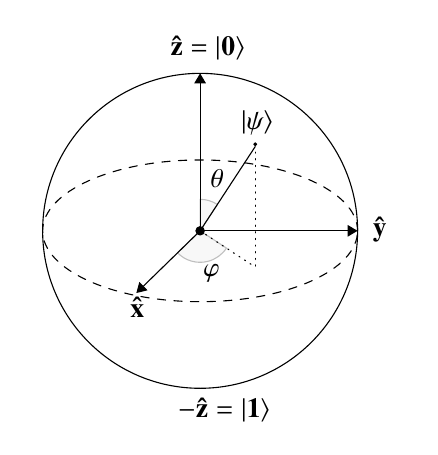
\begin{tikzpicture}[line cap=round, line join=round, >=Triangle]
  \clip(-2.19,-2.49) rectangle (2.66,2.58);
  \draw [shift={(0,0)}, lightgray, fill, fill opacity=0.1] (0,0) -- (56.7:0.4) arc (56.7:90.:0.4) -- cycle;
  \draw [shift={(0,0)}, lightgray, fill, fill opacity=0.1] (0,0) -- (-135.7:0.4) arc (-135.7:-33.2:0.4) -- cycle;
  \draw(0,0) circle (2cm);
  \draw [rotate around={0.:(0.,0.)},dash pattern=on 3pt off 3pt] (0,0) ellipse (2cm and 0.9cm);
  \draw (0,0)-- (0.70,1.07);
  \draw [->] (0,0) -- (0,2);
  \draw [->] (0,0) -- (-0.81,-0.79);
  \draw [->] (0,0) -- (2,0);
  \draw [dotted] (0.7,1)-- (0.7,-0.46);
  \draw [dotted] (0,0)-- (0.7,-0.46);
  \draw (-0.08,-0.3) node[anchor=north west] {$\varphi$};
  \draw (0.01,0.9) node[anchor=north west] {$\theta$};
  \draw (-1.01,-0.72) node[anchor=north west] {$\mathbf {\hat{x}}$};
  \draw (2.07,0.3) node[anchor=north west] {$\mathbf {\hat{y}}$};
  \draw (-0.5,2.6) node[anchor=north west] {$\mathbf {\hat{z}=|0\rangle}$};
  \draw (-0.4,-2) node[anchor=north west] {$-\mathbf {\hat{z}=|1\rangle}$};
  \draw (0.4,1.65) node[anchor=north west] {$|\psi\rangle$};
  \scriptsize
  \draw [fill] (0,0) circle (1.5pt);
  \draw [fill] (0.7,1.1) circle (0.5pt);
\end{tikzpicture}
\caption[Bloch sphere.]{The Bloch sphere is a geometrical representation of the Quantum state in QC.}
\end{figure}

\begin{figure}
\centering
\includegraphics[width=5cm,height=5cm]{./figure/bloch-redfield.png}
\caption[Bloch Sphere]{Bloch Sphere based on Bloch-Redfield master eq.} 
\end{figure}

\begin{figure}
\centering
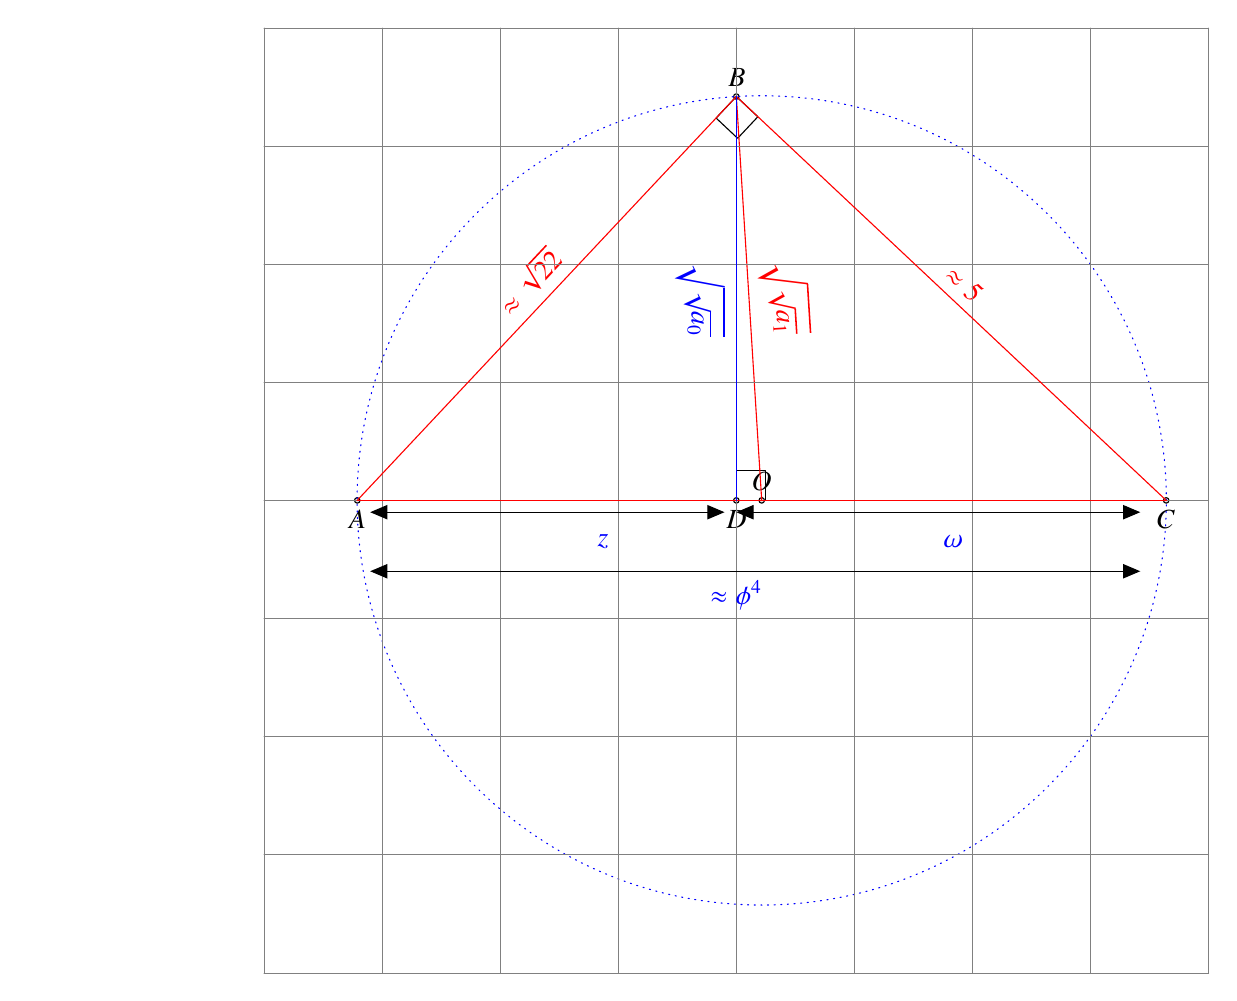
\begin{tikzpicture}[scale=1.5,line cap=round,line join=round,>=triangle 
45,x=1.0cm,y=1.0cm]
%\label{tab:15:table15}
\tkzDefPoint(-3.21,0.0){A} \tkzDefPoint(0.0,3.42){B} \tkzDefPoint(3.64,0.){C} \tkzDefPoint(0.0,0.0){D}
\tkzDrawPoints(A,B,C,D)
\tkzMarkRightAngle(A,B,C)
\tkzMarkRightAngle(B,D,C)
\tkzLabelPoints[below](A,C,D)
\tkzLabelPoints[above](B)
%\tkzMarkAngle[fill=blue!40,size=1.4cm,opacity=.5](C,A,B)
%\tkzLabelAngle[pos=1.6](C,A,B){$\theta$}
\tkzDefMidPoint(A,C) \tkzGetPoint{O}
\coordinate (center) at (O);
\tkzLabelPoints[above](O)
\tkzDrawPoints(O)
\tkzLabelSegment[sloped,above,text=red](A,B){$\approx \sqrt{22}$}
\tkzLabelSegment[sloped,above,text=red](B,C){$\approx 5$}
%\tkzLabelSegment[sloped,below,text=red](A,C){$\approx \phi^{4}$}
\draw[blue, dotted]
      let \p1 =  ($(B)-(center)$),
          \n0 = {veclen(\x1,\y1)}
      in (center) circle(\n0);
\draw[color=red] (B) -- (O);
\tkzDefMidPoint(B,O) \tkzGetPoint{F}
\tkzLabelSegment[sloped,above,text=red](B,O){$\sqrt{\sqrt{a_1}}$}
\draw[color=blue] (B) -- (D);
\tkzDefMidPoint(B,D) \tkzGetPoint{G}
\tkzLabelSegment[sloped,below,text=blue](B,D){$\sqrt{\sqrt{a_0}}$}
\draw[step=1cm,gray,very thin] (-4,-4) grid (4,4);
\draw[color=red] (-3.21,0.) -- (0.,0.);
\draw[color=red] (3.64,0.) -- (0.,0.0);
\draw[color=red] (-3.21,0.) -- (0.,3.42);
\draw[color=red] (0.,3.42) -- (3.64,0.);
\draw[color=blue] (0.,0.) -- (0.,3.42);
%\node [anchor = east] at (0.,1.5) {$\sqrt{\sqrt{a_1}}$};
%\node [anchor = east] at (2.,2.0) {$\approx 5$};
%\node [anchor = east] at (-1.,2.0) {$\approx \sqrt{22}$};
\node [anchor = north,text=blue] at (0.,-0.6) {$\approx \phi^{4}$};
\draw [<->] (-3.1,-0.1) node[left]{} -- (-0.1,-0.1) node[right]{};
\draw [<->] (0.0,-0.1) node[left]{} -- (3.42,-0.1) node[right]{};
\draw [<->] (-3.1,-0.6) node[left]{} -- (3.42,-0.6) node[right]{};
  %\draw [decoration={markings,mark=at position 1 with
   % {\arrow[scale=3,>=stealth reversed]{<}}},postaction={decorate}] (-3.2,-0.3) -- (3.42,-0.3);
\node [anchor = east,text=blue] at (2.,-0.35) {$\omega$};
\node [anchor = east,text=blue] at (-1.,-0.35) {$z$};
\clip(-6.,-0.4) rectangle (0.4,3.4);
%\draw [shift={(-3.2,0.)},color=gray,fill=darkgray,fill opacity=0.1] (0,0) -- (0.:0.6) arc (0.:43.9:0.6) -- cycle;
%\draw[color=gray,fill=darkgray,fill opacity=0.1] (0.,0.42) -- (-0.42,0.42) -- (-0.42,0.) -- (0.,0.) -- cycle; 
%\draw (0.,6.)-- (-4.32,0.);
%\draw (6.,5.52)-- (-4.32,0.);
%\draw (6.,0.)-- (6.,5.52);
%\draw[color=gray] (-3.2,0.4) node {\large $\theta$};
%\draw[color=gray] (0.34,0.33);
%\tkzMarkRightAngle[fill=blue!20](B,F,C)
\end{tikzpicture}
\caption[The Golden Sanchez Triangle.]{Golden Sanchez Triangle.}
\end{figure}

 
 \begin{figure}
\centering
\begin{tikzpicture}[scale=1.25]
%\tkzInit[xmax=6.4, zmax=3.4]
\tkzDefPoint(0.0,0.0){C} \tkzDefPoint(4.9,0.0){B} \tkzDefPoint(3.12,-1.74){A} \tkzDefPoint(1.8,-1.0){q}
\tkzDrawPoints(A,B,C,q)
\tkzDefMidPoint(B,q) \tkzGetPoint{D}
%\tkzDefPoint[label={[text=blue,align=left]right:$z$},xshift=-01mm](2.25,-1.50){F}
%\tkzDefPoint[label={[text=blue,align=left]right:$\omega$},xshift=-01mm](0.75,-0.70){E}
%\tkzDefPoint[label={[text=red,align=left]right:$\sqrt{\omega z}$},xshift=-01mm](2.8,-0.29){D}
%\tkzDefPoint[label={[align=right]right:$4 \cdot \sqrt{(3H\beta/n)}$},xshift=00mm](3.0,-0.79){D}
\tkzLabelSegment[sloped,below,text=red](q,B){$\sqrt{\omega z}$}
\tkzLabelSegment[sloped,below,text=blue](A,q){$z$}
\tkzLabelSegment[sloped,below,text=blue](C,q){$\omega$}
\tkzLabelSegment[sloped,text=blue,xshift=1.5mm,yshift=-07.5mm](A,C){$\phi^4$}
\tkzMarkRightAngle(A,B,C)
\tkzMarkRightAngle(B,q,C)
\tkzLabelPoints[below](A,B,C)
\tkzDrawSegments[red](B,q)
%\tkzLabelPoints[above right](q)
%\tkzMarkAngle[fill=blue!40,size=1.4cm,opacity=.5](C,A,B)
%\tkzLabelAngle[pos=0.6](A,q,B){$\sqrt{\omega z}$}
    %\draw [important line] (0.0,0.) coordinate (A) -- (5.1,-1.3) coordinate (C) node[below, text width=5em] {}
    %\draw [blue] (6.4,0.) coordinate (A) -- (4.,-1.0) coordinate (D) node[below, text width=5em] {$h$}
    %\draw [red] (6.4,0.) coordinate (B) -- (4.,-1.0) coordinate (D) node[below, text width=5em] {$q$}
  \draw (4.9,0,0) coordinate (x) |- (0,1,0) coordinate [midway] (h) coordinate (y) -- (0,1,4.6) coordinate (a) -- (0,0,4.6) coordinate (z) -- (4.9,0,4.6) edge (x) -- (4.9,1,4.6) coordinate (v) edge (h)
  -- (a)  ;
  \draw [dashed] (0,0,0) coordinate (o) edge (x) edge (y) -- (z);
  \draw [dashed] (0,0,0) coordinate (o) edge (x) edge (v) -- (v);
  \draw [blue] (0,0,0)  -- (4.9,0.0,4.6);
  \draw [very thin,black,line join=round] (0,0,0)  -- node [sloped,above,xshift=-0.mm,yshift=-2.mm] {$\approx 4\sqrt 3$} (4.9,1.,4.6);
  %\node [circle, minimum size=2pt, inner sep=0pt, fill, label=135:$4 \cdot \sqrt{(3H\beta/n)}$] at (v) {};
  \node [circle, minimum size=4pt, inner sep=0pt, fill, label=135:o] at (o) {};
  \draw [decoration={markings,mark=at position 1 with
    {\arrow[scale=3,>=stealth]{>}}},postaction={decorate}] (0,0,0) -- (4.9,1,4.6);
  %\draw [<->] (0.2,-0.5) node[left]{} -- (2.2,-1.8) node[below]{$\phi^4$};
  \draw [->] (x) -- +(3pt,0,0) node [midway,above] {$\sqrt{\omega \cdot (\omega+z)}$};
  \draw [->] (y) -- +(0,3pt,0) node [midway,right] {$1$};
  \draw [->] (z) -- +(0,0,3pt) node [midway,above] {$\sqrt{z \cdot (\omega+z)}$};
  %\draw (v) -- ++(0,0,-2) coordinate (d) -- ++(-2,0,0) coordinate (e) -- ++(0,0,2) |- ++(2,-2,0) coordinate [midway] (f) -- ++(0,0,-2) coordinate (g) -- (d);
  %\draw [dashed] (e) -- ++(0,-2,0) coordinate (c) edge (f) -- (g);
  %\node [label=45:C] at (c) {};
  %\draw[red]   (0,0,0) -- (.95,0,0)    node[red,left=6pt]    {$x$};
\end{tikzpicture}
\caption[The Golden Sanchez cuboid properties]{3D perspective of the "Golden-Sanchez" cuboid: Electro-weak / Eddington matrix connection}
\end{figure}






\begin{table}
%\label{tab:2:table2}
\caption[Table \ref{tab:2:table2}: Adimensional primary constants.]{Adimensional primary constants}
\label{tab:2:table2}
  \hskip-2.0cm\begin{tabular}{llll}
    \toprule
    %\multicolumn{4}{c}{}                   \\
    \cmidrule(r){1-4}
    name & symbol    & value & imp (ppb) \\
    \midrule
    
    Euler-Napier constant  & e    & 2.718281828459042 & "exact" \\    
    Archimedes constant & $\pi$    & 3.14159265358979 & "exact" \\    
    %$\pi$ fifth fractional term & $\pi_5$    & 292.63459101440 & "exact" \\ 
    Euler-Mascheroni constant & $\gamma$    & 0.57721566490153 & "exact" \\    
    %Wien factor $ w_i = 5(1-e^{-w_i})$ &  $w_i$  & 4.96514245  & "exact" \\
     
    Electric coupling constant  & $a$    & 137.035999084(21) & 0.15 \\
    Excess Electron Magnetic moment  & $d_e$    & 1.00115965218128 & 0.15 ppb \\
    Atiyah constant & $\Gamma= \gamma a/\pi$    & 25.17809724196  & 0.15 ppb \\ 
    %Measured massive scalar boson/Electron mass ratio  & $H^0_{meas}$ & 245000(250)  & $10^6$ \\
    Optimized massive scalar boson/Electron mass ratio  & $H^{(0)}$ & $ 495^2 = 245025$  & exact, $H^{(0)}_{mes}$: 245000(250)  \\
    
    %Measured W boson/Electron mass ratio  & $W_{meas}$ &   & $1.5 \times 10^5$ \\     
    Optimized  charged weak  boson/Electron mass ratio  & $W$ & 157340.1093  & ppb\cite{Sanchez2} $W_{mes}$: 157297(24)  \\     
    %This work  W boson/Electron mass ratio  & $W$ & 157340.1100  & ppb \\
    
    %Measured Z boson/Electron mass ratio  & $Z_{meas}$ & 178450(4)  & $2.3 \times 10^4$ \\     
    Optimized  neutral weak boson/Electron mass ratio  & $Z$ & 178451.7524  & ppb\cite{Sanchez2} $Z_{mes}$: 178450(4)\\     
   %This work  Z boson/Electron mass ratio  & $Z$ & 178451.7171  & ppb\\
   
  %Effective "weak-mixing angle"  & $(\sin \theta)^2(m_Z)$    & 0.23155(4) & $1.7 \times 10^7$ \\
  %This work "weak-mixing angle" & $(\sin \theta)^2(m_Z)$    & 0.231475 &  \\
  
  
  
 DNA Adenine-Thymine couple principal mass/$m_H$ &  $o_1$   & 612.31268  & \cite{Huang} \\
 DNA Guanine-Cytosine couple principal mass/$m_H$ &  $o_2$   & 613.300194  & \cite{Huang} \\ 
  
  
   %Optimized SU(2) gauge coupling &  $g_2$   & 0.6421390 & 100 this work \\
   %Optimized U(1) gauge coupling & $g_1$   & 0.3436257 & 100 this work \\
   %Optimized electric charge & $ q $    & 0.3029732 & 100 this work\\
   
   %"Squared Weak-mixing angle"  & $(\sin \theta_Z)^2$    & 0.23122(4) & $1.7 \times 10^7$ \\
  
   %Optimized "m(Z) Squared Weak-mixing angle" $qR/R_N$  & $(\sin \theta_Z)^2$    & 0.2311293 & this work, (0.23122(4)) \\
   
  %Effective "Squared m(Z) Weak-mixing angle"  & $(\sin \theta_{effZ})^2$    & 0.23148(4) & $1.7 \times 10^7$ \\
  
   %Optimized "Effective m(Z) Squared Weak-mixing angle" $(ln\Phi)^2$  & $(\sin \theta_{effZ})^2$    & 0.23156482 & this work (0.23148(4)) \\
                         
    Lucas Large Prime Number & $N_L$    & $2^{127}-1$  & exact \\
    Eddington Large Number & $N_{Ed}$    & $136\times 2^{256}$  & exact \\
    Monster Group order  & $O_{M}$    & $ exp {124.1264234...}$  & exact \\
    %Measured Fermi/Electron $m_F/m_e$ & $F_{meas}$   & 573007.362  & 250 \\ 
          
    Proton/Electron mass ratio $m_p/m_e$ & p   & 1836.15267343  & 0.06 \\  
    Hydrogen/Electron mass ratio  & $H$  & 1837.15266014  & 0.06 \\
    Relativistic correction factor $1/(H-p)$ & $\beta$  & 1.000026597  & 0.1 \\
    Neutron/Electron mass ratio  & $n_t$ & 1838.6836617  & 0.5 \\     
    %Measured Muon/Electron mass ratio  & $\mu_{meas}$ & 206.7682830  & 22 \\     
    Optimized Muon/Electron mass ratio  & $\mu$ & 206.7682869  & 0.1 $\mu_{mes}$: 206.7682830 \\     
   % Measured Tau/Electron mass ratio  & $\tau_{meas}$ & 3477(2)  & $7\times 10^4$ \\        
    Optimized Koide Tau ratio $p_K = (1+\mu+\tau)\/2 = (1+\sqrt \mu+\sqrt\tau)^2/3 \approx \beta\tau ln17/ln210$     & $\tau$ & 3477.441701  & 0.1 $\tau_{mes}$: 3477(2) \\  
 Fermi Sanchez-Atiyah mass ratio: & $F$   & 573007.3652  & 0.22 $F_{mes}$: 573007.362 \\
 Planck ratio $m_P/m_e$ & P   & $2.389015907 \times 10^{22}$ &ppb  \cite{Sanchez2}  \\
 Gravitational proton ratio $P N_L^{-1/2}$ & $p_G$    & $ 1831.531181 $ &ppb  \cite{Sanchez2}  \\
 Gravitational coupling constant $R/2\lambdabar_e = P^2/pH$ & $a_G$   & $1.691936467 \times 10^{38}$ &ppb  \cite{Sanchez2}  \\
 Electroweak coupling constant $F^2 = (2\gamma\times 137)^3$ & $a_w$     & $3.283374406 \times 10^{11}$ & ppb \cite{Sanchez2}  \\
Optimised Strong coupling constant $a_w/2\pi(pH)^{3/2}$ & $a_s$   & $8.434502906$ & ppb \cite{Sanchez2} $a_{s(mes)}$:8.47(7) \\
 Scale-factor $8\pi^2/ln2$  & $j$ & 113.9106346  & \cite{Sternheimer} \\
 
   
    
         
   \bottomrule
  \end{tabular}
\end{table}
 
 
 \begin{table}
%\label{tab:3:table3}
\caption[Table \ref{tab:3:table3}: Physical constants]{Table of Physical constants}
\label{tab:3:table3}
  \hskip-2.0cm\begin{tabular}{lllll}
    \toprule
    %\multicolumn{5}{c}{}                  \\
    \cmidrule(r){1-5}
    \ name & Symbol  & unit  & Value & imprecision (ppb) \\
    \midrule
  
 
 Reduced Planck constant $h/2\pi$    & $\hbar$   & J s   & $1.05457181 \times 10^{-34}$ & "exact" \\
 %Official Gravitation constant   & $G_{off}$ & $kg^{-1} m^3 s^{-1}$ & $6.67430 \times 10^{-11}$  &  contested\\
 Optimized Gravitation constant   & G & $kg^{-1} m^3 s^{-1}$  & $6.67545375\times 10^{-11}$  & \cite{Sanchez2} $G_{mes}$: 6.67430 \\
 Relativity speed     & c   & $m s^{-1}$   & 299792458 & exact \\
 Fermi constant  & $G_F$ & $J m^3$   & $61.435851 \times 10^{-62}$  &  500\\
 Electron mass $m_e = m_p/p = m_H/H = m_n/n_t$  & $m_e$ & kg  & $9.1093837015 \times 10^{-31}$  &  0.3\\
 Electron reduced wavelength $\hbar/m_ec$ & $\lambdabar_e$ &  m   & $3.861592675\times 10^{-13}$  & 0.3\\
 Electron classical radius $\hbar/am_ec$ & $r_e$ &  m   & $2.817940322\times 10^{-15}$  & 0.45\\
 Hydrogen Bohr radius $a(1+1/p)\lambdabar_e$ & $r_H$ &  m   & $5.294654092 \times 10^{-15}$  & 0.45\\
 %Proton radius  & $r_p$ &  m   & $8.8\times 10^{-16}$  & contested\\
 %Planck length $(\hbar G /c^3)^{1/2}$ & $l_P$  & m  & $1.61639471 \times 10^{-35}$ & ppb \cite{Sanchez2}  \\
 
 %Rydbergh reduced wavelength $\lambdabar_e(2aH/p)^2$ & $\lambdabar_{Ryd}$  & m  & $1.45190673 \times 10^{-8} $ & 0.3   \\
 
 
 
  %Official CMB temperature & $T_{CMBoff}$ & K & $2.7255(6)$ & $2 \times 10^5$ \\    
   Cosmos (CMB) temperature & $T_{C}$ & K & $2.725820138$ & \cite{Sanchez2}, $T_{CMB(mes)} $ 2.7255(6)  \\
   Cosmos (CMB) reduced wavelength & $\lambdabar_{CMB} = \hbar c/ k_B T_C $ & m & $8.400716621 \times 10^{-4} $ & \cite{Sanchez2} \\
   Cosmos (CMB) Wien wavelength & $\lambda_{CMB}/w_i $ & m & $1.063082472  \times 10^{-3} $ & \cite{Sanchez2} \\
   %Neutrino (CNB) reduced wavelength & $\lambdabar_{CNB} = \lambdabar_{CNB} \times (11/4)^{1/3}  $ & m & $1.176956919 \times 10^{-3} $ & \cite{Sanchez2} \\
   
   Non-Local length & $l_{nl}$ & m & $2.878184911 \times 10^{12} $ & \cite{Sanchez2} \\ 
   
    Hubble length (Universe radius) & $R$ & m & $1.306713894 \times 10^{26} $ & \cite{Sanchez2} \\ 
   Mono-electron Universe radius & $R_1$ & m & $1.492365473 \times 10^{26} $ & \cite{Sanchez2} \\ 
   Cosmos holographic radius & $R_N$ & m & $1.712894163 \times 10^{26} $ & \cite{Sanchez2} \\
    Cosmos radius & $ R_C$ & m & $9.075773376 \times 10^{86} $ & \cite{Sanchez2} \\
   Universe mass & $M$ & kg & $8.7965248 \times 10^{52} $ & \cite{Sanchez2} \\ 
   Cosmos holographic mass & $M_N = M'$ & kg & $1.15308454 \times 10^{53} $ & \cite{Sanchez2} \\
 
   Cosmos mass & $M_C$ & kg & $2.247604 \times 10^{113} $ & \cite{Sanchez2} \\ 
   

    \bottomrule
  \end{tabular}
\end{table}
















%\bibitem{Hirzebruch} Hirzebruch F. Topological methods in algebraic geometry. Springer 1966.\\
%\bibitem{Bott} M. Atiyah, R. Bott, V. Patodi, "On the heat equation and the index theorem" Invent. Math. , 19 (1973) pp. 279--330.\\
%\bibitem{Singer} M. Atiyah, I. Singer, "The index of elliptic operators IV" Ann. of Math. , 93 (1971) pp. 119--138. \\
%\bibitem{Alvarez} L. Alvarez-Gaume, "Supersymmetry and the Atiyah Singer index theorem" Comm. Math. Phys. , 90 (1983) pp. 161--170.\\


%\bibitem{Frenkel} I. B. Frenkel, J. Lepowsky, and A. Meurman, “A Natural Representation of the Fischer-Griess Monster With the Modular Function J As Character,” Proc. Natl. Acad. Sci. USA 81 (1984) 3256-3260. 

%\bibitem{Witten} Witten E., Three-Dimensional Gravity Revisited arxiv.org/abs/0706.3359 



%\bibitem{deVries} Hans de Vries. http://www.chip-architect.com/news/2004/10/04. The Electro-Magnetic coupling constant.html, An exact formula for the Electro Magnetic coupling constant, web page, 2004 Oct 4.\\ 


%\bibitem{Atiyah1} Atiyah M. Private Communication (december 2018).\\

%\bibitem{Conway} Conway, John Horton; Norton, Simon P. (1979). "Monstrous Moonshine". Bull. London Math. Soc. 11 (3): 308--339.\\
%\bibitem{Borcherds} Borcherds, Richard (1992), "Monstrous Moonshine and Monstrous Lie Superalgebras", Invent. Math., 109: 405--444.\\

%\bibitem{Shannon} Shannon C.E. « A Mathematical Theory of Communication » Reprinted with corrections from The Bell System Technical Journal, Vol. 27, p. 379–423, 623–656, July, October, 1948.)\\
%\bibitem{Stark} Stark H.M. A complete determination of the complex quadratic fields of class-number one, Michigan Math. J., vol. 14,‎ 1967, p. 1-27  \\
%\bibitem{Lovelace} Lovelace C. (1971) Pomeron form factors and dual Regee cuts, Physics Letters B34 (6) 500-506.\\
%\bibitem{Apostol} Apostol T. Modular functions and Dirichlet Series in Number Theory. Springler-Verlag. New-York (1990).\\

%\bibitem{Shlay} Shray J. (1994) Octonions and Supersymmetry, PhD thesis.  http://ir.library.oregonstate.edu/xmlui/handle/1957/35649. \\
 
%\bibitem{Hooft} Hooft 't Th Holographic Principle. ArXiv: hep-th/003004 (2000). \\
%\bibitem{Bousso} Bousso R., The Holographic Principle, Review of Modern Physics, vol 74, p.834 (2002).\\
 
%\bibitem{Durham} Durham I.T. 2006, Sir Arthur Eddington and the Foundations of Modern Physics arXiv:quant-ph/0603146v1  p.117.
%\bibitem{Sanchez2} Sanchez F.M., Kotov V. and Bizouard C., 'Towards a synthesis of two cosmologies: the steady- state flickering Universe'. Journal of Cosmology, vol 17. (2011).\\


%\bibitem{Carr} Carr B.J. and Rees M. J. , “The anthropic principle and the structure of the physical world”, Nature 278, 605-612 (1979).\\
%\bibitem{Sanchez3} F.M. Sanchez. Coherent Cosmology Vixra.org,1601.0011. Springer International Publishing AG 2017. A. Tadjer et al. (eds.), Quantum Systems in Physics, Chemistry, and Biology, Progress in Theoretical Chemistry and Physics 30, pp. 375--407. \\ 
%\bibitem{LaGuer} Gueroult.L, 49 methods for computing the Hubble Radius with Jupyter https://mybinder.org/v2/gh/LaGuer/hubble-radius/master \\

%\bibitem{Lenz} Friedrich Lenz, The Ratio of Proton and Electron Masses, Phys. Rev. 82, 554 - 1951.\\

%\bibitem{Lecompte} Sanchez, F and Lecompte, C, ``Q-Switched $Nd^{3+}$ Glass Laser of Variable Temporal Coherence, Applied optics'', vol.13, p1071-6, 05.1974, DOI: 10.1364/AO.13.001071 \\


%\bibitem{Mainfray} Lecompte, C. and Mainfray, G. and Manus, C. and Sanchez, F., ``Laser temporal-coherence effects on multiphoton ionization processes'', Phys. Rev. A, vol.11, 03.1975, DOI: 10.1103/PhysRevA.11.1009 \\

%\bibitem{Manus} Mainfray, G. and Manus, C. and Sanchez, F., ``Experimental Demonstration of Laser Temporal Coherence Effects on Multiphoton Ionization Processes'', Quantum Electronics, IEEE Journal of, vol.QE10, p707, 10.1974, DOI:0.1109/JQE.1974.1068290 \\


%\bibitem{SanchezF} Sanchez, F., ``High-order multimode radiation statistics of aTEM00Q-switched neodymium laser'', Il Nuovo Cimento B, vol.27, p305--322, 06.1975, DOI:10.1007/BF02738949 \\


%\bibitem{Nist} ``2018 CODATA Value: Newtonian constant of gravitation''. The NIST Reference on Constants, Units, and Uncertainty. NIST. 20 May 2019. Retrieved 20 May 2019. https://www.physics.nist.gov/cgi-bin/cuu/Value?bg \\

%\bibitem{Haramein} Haramein N. ``The Schwarzschild Proton'', 2011, p95--100, vol.60, DOI: 10.1063/1.3527190. \\

%\bibitem{Haramein} Haramein N., Val Baker A. ``Resolving the Vacuum catastrophe. A Generalised Holographic Approach. Journal of High Energy Physics, Gravitation and Cosmology'', 2019, 5, 412-424 \\ 

%\bibitem{Val} Val Baker A. ``The puzzle of the proton'', DOI : 1031219/osf.io/myfxh \\

%\bibitem{Maruani} Jean Maruani. ``The Dirac Electron: From Quantum Chemistry to Holistic Cosmology'' in Journal of the Chinese Chemical Society, vol.63 issue 1, Taipei, Wiley VCH Verlag GmbH, 2016, 33--48 p. DOI: https://doi.org/10.1002/jccs.201500374 \\

%\bibitem{oeis1} OEIS Foundation Inc. The on-line encyclopedia of integer sequences,https://oeis.org/A180873, Sep 22 2010.

%\bibitem{Veysseyre} Veysseyre R., Veysseyre H., and Weigel D. "Nombre de types d’opérations ponctuelles de symétrie cristallographiques dans l'espace E^{n} . (Number of types of crystallographic point symmetry operations of space E^{n} )", Comptes Rendus de l’Académie des Sciences. Série II (Jan.1990).\\

%\bibitem{Weigel} Veysseyre R., Veysseyre H., and Weigel D. "Counting, types and symbols of crystallographic Point Symmetry Operations of space E n" AAECC 5, 53–70 (1992) DOI: 10.1007/BF01196625 ISBN: 0938-1279.\\



